%%%%%%%%%%%%%%%%%%%%%%%%%%%%% Thesis.tex %%%%%%%%%%%%%%%%%%%%%%%%%%%%%%%
%                                                                      %
%  ---------- Master of Science Dissertation template ----------       %
%                                                                      %
%  Template for the Master Thesis according to the regulations         %
%  published by the Scientific Council at IST.                         %
%                                                                      %
%  For up-to-date regulations, please refer to                         %
%  http://cd.ist.utl.pt/files/publico/academicos/guia_dissertacao.pdf  %
%                                                                      %
%       Andre C. Marta                                                 %
%       Area Cientifica de Mecanica Aplicada e Aeroespacial            %
%       Departamento de Engenharia Mecanica                            %
%       Instituto Superior Tecnico                                     %
%       Av. Rovisco Pais                                               %
%       1049-001 Lisboa                                                %
%       Portugal                                                       %
%       Tel: +351 21 841 9466                                          %
%                        3466 (extension)                              %
%       Email: andre.marta@ist.utl.pt                                  %
%                                                                      %
%  Created:       Jan 20, 2011                                         %
%  Last Modified: Jan 24, 2011                                         %
%                                                                      %
%%%%%%%%%%%%%%%%%%%%%%%%%%%%%%%%%%%%%%%%%%%%%%%%%%%%%%%%%%%%%%%%%%%%%%%%
%                                                                      %
% To generate the PDF file, type "make" at the terminal prompt.        %
%                                                                      %
% The IST template LaTeX package was created by the author             %
% and it can be downloaded from:                                       %
% https://fenix.ist.utl.pt/homepage/ist31052/                          %
%                                                                      %
% The external packages can be downloaded from                         %
% the Comprehensive TeX Archive Network at http://www.ctan.org/        %
%                                                                      %
% List of LaTex symbols:                                               %
% http://www.ctan.org/tex-archive/info/symbols/comprehensive/          %
%                                                                      %
% Help with LaTex can be found at                                      %
% http://www.giss.nasa.gov/tools/latex/ltx-2.html                      %
% http://en.wikibooks.org/wiki/LaTeX                                   %
%%%%%%%%%%%%%%%%%%%%%%%%%%%%%%%%%%%%%%%%%%%%%%%%%%%%%%%%%%%%%%%%%%%%%%%%

%%%%%%%%%%%%%%%%%%%%%%%%%%%%%%%%%%%%%%%%%%%%%%%%%%%%%%%%%%%%%%%%%%%%%%%%
%     Preamble                                                         %
%%%%%%%%%%%%%%%%%%%%%%%%%%%%%%%%%%%%%%%%%%%%%%%%%%%%%%%%%%%%%%%%%%%%%%%%

% ----------------------------------------------------------------------
%  Set the document class
% ----------------------------------------------------------------------
\documentclass[10pt,a4paper,twoside]{report}

% ----------------------------------------------------------------------
% Define external packages, language, margins, fonts and new commands
% ----------------------------------------------------------------------
%%%%%%%%%%%%%%%%%%%%%%%%%%%%%%%%%%%%%%%%%%%%%%%%%%%%%%%%%%%%%%%%%%%%%%%%
%                                                                      %
%     File: Thesis_Preamble.tex                                        %
%     Tex Master: Thesis.tex                                           %
%                                                                      %
%     Author: Andre C. Marta                                           %
%     Last modified : 24 Jan 2011                                      %
%                                                                      %
%%%%%%%%%%%%%%%%%%%%%%%%%%%%%%%%%%%%%%%%%%%%%%%%%%%%%%%%%%%%%%%%%%%%%%%%

% ----------------------------------------------------------------------
% Define document language.
% ----------------------------------------------------------------------

% 'inputenc' package
%
% Accept different input encodings.
% http://www.ctan.org/tex-archive/macros/latex/base/
%
% > allows typing non-english text in LaTeX sources.
%
% ******************************* SELECT *******************************
%\usepackage[latin1]{inputenc} % <<<<< Windows
\usepackage[utf8]{inputenc}   % <<<<< Linux
% ******************************* SELECT *******************************


% 'babel' package
%
% Multilingual support for Plain TeX or LaTeX.
% http://www.ctan.org/tex-archive/macros/latex/required/babel/
%
% > sets the variable names according to the language selected
%
% ******************************* SELECT *******************************
%\usepackage[portuguese]{babel} % <<<<< Portuguese
\usepackage[english]{babel} % <<<<< English
% ******************************* SELECT *******************************


% List of LaTeX variable names: \abstractname, \appendixname, \bibname,
%   \chaptername, \contentsname, \listfigurename, \listtablename, ...)
% http://www.tex.ac.uk/cgi-bin/texfaq2html?label=fixnam
%
% Changing the words babel uses (uncomment and redefine as necessary...)
%
\newcommand{\acknowledgments}{@undefined} % new LaTeX variable name
%
% > English
%
\addto\captionsenglish{\renewcommand{\acknowledgments}{Acknowledgments}}
%\addto\captionsenglish{\renewcommand{\listtablename}{List of Tables}}
%\addto\captionsenglish{\renewcommand{\listfigurename}{List of Figures}}
%\addto\captionsenglish{\renewcommand{\nomname}{Nomenclature}}
%\addto\captionsenglish{\renewcommand{\appendixname}{Appendix}}
%\addto\captionsenglish{\renewcommand{\bibname}{References}} % Bibliography

% > Portuguese
%
\addto\captionsportuguese{\renewcommand{\acknowledgments}{Agradecimentos}}
%\addto\captionsportuguese{\renewcommand{\listtablename}{Lista de Figuras}}
%\addto\captionsportuguese{\renewcommand{\listfigurename}{Lista de Tabelas}}
%\addto\captionsportuguese{\renewcommand{\nomname}{Lista de S\'{i}mbolos}} % Nomenclatura
%\addto\captionsportuguese{\renewcommand{\appendixname}{Anexo}} % Apendice
%\addto\captionsportuguese{\renewcommand{\bibname}{Refer\^{e}ncias}} % Bibliografia


% ----------------------------------------------------------------------
% Define default and cover page fonts.
% ----------------------------------------------------------------------

% Use Arial font as default
%
\renewcommand{\rmdefault}{phv}
\renewcommand{\sfdefault}{phv}

% Define cover page fonts
%
%         encoding     family       series      shape
%  \usefont{T1}     {phv}=helvetica  {b}=bold    {n}=normal
%                   {ptm}=times      {m}=normal  {sl}=slanted
%                                                {it}=italic
% see more examples at
% http://julien.coron.free.fr/languages/latex/fonts/
%
\def\FontLn{% 16 pt normal
  \usefont{T1}{phv}{m}{n}\fontsize{16pt}{16pt}\selectfont}
\def\FontLb{% 16 pt bold
  \usefont{T1}{phv}{b}{n}\fontsize{16pt}{16pt}\selectfont}
\def\FontMn{% 14 pt normal
  \usefont{T1}{phv}{m}{n}\fontsize{14pt}{14pt}\selectfont}
\def\FontMb{% 14 pt bold
  \usefont{T1}{phv}{b}{n}\fontsize{14pt}{14pt}\selectfont}
\def\FontSn{% 12 pt normal
  \usefont{T1}{phv}{m}{n}\fontsize{12pt}{12pt}\selectfont}


% ----------------------------------------------------------------------
% Define page margins and line spacing.
% ----------------------------------------------------------------------

% 'geometry' package
%
% Flexible and complete interface to document dimensions.
% http://www.ctan.org/tex-archive/macros/latex/contrib/geometry/
%
% > set the page margins (2.5cm minimum in every side, as per IST rules)
%
\usepackage{geometry}	
\geometry{verbose,tmargin=2.5cm,bmargin=2.5cm,lmargin=2.5cm,rmargin=2.5cm}

% 'setspace' package
%
% Set space between lines.
% http://www.ctan.org/tex-archive/macros/latex/contrib/setspace/
%
% > allow setting line spacing (line spacing of 1.5, as per IST rules)
%
\usepackage{setspace}
\renewcommand{\baselinestretch}{1.5}


% ----------------------------------------------------------------------
% Include external packages.
% Note that not all of these packages may be available on all system
% installations. If necessary, include the .sty files locally in
% the <jobname>.tex file directory.
% ----------------------------------------------------------------------

% 'graphicx' package
%
% Enhanced support for graphics.
% http://www.ctan.org/tex-archive/macros/latex/required/graphics/
%
% > extends arguments of the \includegraphics command
%
\usepackage{graphicx}


% 'color' package
%
% Colour control for LaTeX documents.
% http://www.ctan.org/tex-archive/macros/latex/required/graphics/
%
% > defines color macros: \color{<color name>}
%
%\usepackage{color}


% 'amsmath' package
%
% Mathematical enhancements for LaTeX.
% http://www.ctan.org/tex-archive/macros/latex/required/amslatex/
%
% > American Mathematical Society plain Tex macros
%
\usepackage{amsmath}  % AMS mathematical facilities for LaTeX.
\usepackage{amsthm}   % Typesetting theorems (AMS style).
\usepackage{amsfonts} % 


% 'wrapfig' package
%
% Produces figures which text can flow around.
% http://www.ctan.org/tex-archive/macros/latex/contrib/wrapfig/
%
% > wrap figures/tables in text (i.e., Di Vinci style)
%
% \usepackage{wrapfig}


% 'subfigure' package
%
% Deprecated: Figures divided into subfigures.
% http://www.ctan.org/tex-archive/obsolete/macros/latex/contrib/subfigure/
%
% > subcaptions for subfigures
%
\usepackage{subfigure}


% 'subfigmat' package
%
% Automates layout when using the subfigure package.
% http://www.ctan.org/tex-archive/macros/latex/contrib/subfigmat/
%
% > matrices of similar subfigures
%
\usepackage{subfigmat}


% 'url' package
%
% Verbatim with URL-sensitive line breaks.
% http://www.ctan.org/tex-archive/macros/latex/contrib/url/
%
% > URLs in BibTex
%
% \usepackage{url}


% 'varioref' package
%
% Intelligent page references.
% http://www.ctan.org/tex-archive/macros/latex/required/tools/
%
% > smart page, figure, table and equation referencing
%
%\usepackage{varioref}


% 'dcolumn' package
%
% Align on the decimal point of numbers in tabular columns.
% http://www.ctan.org/tex-archive/macros/latex/required/tools/
%
% > decimal-aligned tabular math columns
%
\usepackage{dcolumn}
\newcolumntype{d}{D{.}{.}{-1}} % column aligned by the point separator '.'
\newcolumntype{e}{D{E}{E}{-1}} % column aligned by the exponent 'E'


% '' package
%
% Reimplementation of and extensions to LaTeX verbatim.
% http://www.ctan.org/tex-archive/macros/latex/required/tools/
%
% > provides the verbatim environment (\begin{verbatim},\end{verbatim})
%   and a comment environment (\begin{comment},  \end{comment})
%
% \usepackage{verbatim}


% 'moreverb' package
%
% Extended verbatim.
% http://www.ctan.org/tex-archive/macros/latex/contrib/moreverb/
%
% > supports tab expansion and line numbering
%
% \usepackage{moreverb}



% 'nomencl' package
%
% Produce lists of symbols as in nomenclature.
% http://www.ctan.org/tex-archive/macros/latex/contrib/nomencl/
%
% The nomencl package makes use of the MakeIndex program
% in order to produce the nomenclature list.
%
% Nomenclature
% 1) On running the file through LATEX, the command \makenomenclature
%    in the preamble instructs it to create/open the nomenclature file
%    <jobname>.nlo corresponding to the LATEX file <jobname>.tex and
%    writes the information from the \nomenclature commands to this file.
% 2) The next step is to invoke MakeIndex in order to produce the
%    <jobname>.nls file. This can be achieved by making use of the
%    command: makeindex <jobname>.nlo -s nomencl.ist -o <jobname>.nls
% 3) The last step is to invoke LATEX on the <jobname>.tex file once
%    more. There, the \printnomenclature in the document will input the
%    <jobname>.nls file and process it according to the given options.
%
% http://www-h.eng.cam.ac.uk/help/tpl/textprocessing/nomencl.pdf
%
\usepackage{nomencl}
\makenomenclature
%
% Group variables according to their symbol type
%
\RequirePackage{ifthen} 
\ifthenelse{\equal{\languagename}{english}}%
    { % English
    \renewcommand{\nomgroup}[1]{%
      \ifthenelse{\equal{#1}{R}}{%
        \item[\textbf{Roman symbols}]}{%
        \ifthenelse{\equal{#1}{G}}{%
          \item[\textbf{Greek symbols}]}{%
          \ifthenelse{\equal{#1}{S}}{%
            \item[\textbf{Subscripts}]}{%
            \ifthenelse{\equal{#1}{T}}{%
              \item[\textbf{Superscripts}]}{}}}}}%
    }{% Portuguese
    \renewcommand{\nomgroup}[1]{%
      \ifthenelse{\equal{#1}{R}}{%
        \item[\textbf{Simbolos romanos}]}{%
        \ifthenelse{\equal{#1}{G}}{%
          \item[\textbf{Simbolos gregos}]}{%
          \ifthenelse{\equal{#1}{S}}{%
            \item[\textbf{Subscritos}]}{%
            \ifthenelse{\equal{#1}{T}}{%
              \item[\textbf{Sobrescritos}]}{}}}}}%
    }%


%
% Acronimos
%
\usepackage{acronym} 



% 'rotating' package
%
% Rotation tools, including rotated full-page floats.
% http://www.ctan.org/tex-archive/macros/latex/contrib/rotating/
%
% > show wide figures and tables in landscape format:
%   use \begin{sidewaystable} and \begin{sidewaysfigure}
%   instead of 'table' and 'figure', respectively.
%
\usepackage{rotating}


% 'hyperref' package
%
% Extensive support for hypertext in LaTeX.
% http://www.ctan.org/tex-archive/macros/latex/contrib/hyperref/
%
% > Extends the functionality of all the LATEX cross-referencing
%   commands (including the table of contents, bibliographies etc) to
%   produce \special commands which a driver can turn into hypertext
%   links; Also provides new commands to allow the user to write adhoc
%   hypertext links, including those to external documents and URLs.
%
\usepackage[pdftex]{hyperref} % enhance documents that are to be
                              % output as HTML and PDF
\hypersetup{colorlinks,       % color text of links and anchors,
                              % eliminates borders around links
%            linkcolor=red,    % color for normal internal links
            linkcolor=black,  % color for normal internal links
            anchorcolor=black,% color for anchor text
%            citecolor=green,  % color for bibliographical citations
            citecolor=black,  % color for bibliographical citations
%            filecolor=magenta,% color for URLs which open local files
            filecolor=black,  % color for URLs which open local files
%            menucolor=red,    % color for Acrobat menu items
            menucolor=black,  % color for Acrobat menu items
%            pagecolor=red,    % color for links to other pages
%            pagecolor=black,  % color for links to other pages
%            urlcolor=cyan,    % color for linked URLs
            urlcolor=black,   % color for linked URLs
	          bookmarks=true,         % create PDF bookmarks
	          bookmarksopen=false,    % don't expand bookmarks
	          bookmarksnumbered=true, % number bookmarks
	          pdftitle={Thesis},
            pdfauthor={Carlos E. H. J. Fonseca},
            pdfsubject={Eagle Eye},
            pdfkeywords={},
            pdfstartview=FitV,
            pdfdisplaydoctitle=true}


% 'hypcap' package
%
% Adjusting the anchors of captions.
% http://www.ctan.org/tex-archive/macros/latex/contrib/oberdiek/
%
% > fixes the problem with hyperref, that links to floats points
%   below the caption and not at the beginning of the float.
%
\usepackage[figure,table]{hypcap}


% 'natbib' package
%
% Flexible bibliography support.
% http://www.ctan.org/tex-archive/macros/latex/contrib/natbib/
%
% > produce author-year style citations
%
% \citet  and \citep  for textual and parenthetical citations, respectively
% \citet* and \citep* that print the full author list, and not just the abbreviated one
% \citealt is the same as \citet but without parentheses. Similarly, \citealp is \citep without parentheses
% \citeauthor
% \citeyear
% \citeyearpar
%
%\usepackage{natbib}


% ----------------------------------------------------------------------
% Define new commands to assure consistent treatment throughout document
% ----------------------------------------------------------------------

\newcommand{\ud}{\mathrm{d}}                % total derivative
\newcommand{\degree}{\ensuremath{^\circ\,}} % degrees

% Abbreviations

\newcommand{\mcol}{\multicolumn}            % table format

\newcommand{\eqnref}[1]{(\ref{#1})}
\newcommand{\class}[1]{\texttt{#1}}
\newcommand{\package}[1]{\texttt{#1}}
\newcommand{\file}[1]{\texttt{#1}}
\newcommand{\BibTeX}{\textsc{Bib}\TeX}

% Typefaces ( example: {\bf Bold text here} )
%
% > pre-defined
%   \bf % bold face
%   \it % italic
%   \tt % typewriter
%
% > newly defined
\newcommand{\tr}[1]{{\ensuremath{\textrm{#1}}}}   % text roman
\newcommand{\tb}[1]{{\ensuremath{\textbf{#1}}}}   % text bold face
\newcommand{\ti}[1]{{\ensuremath{\textit{#1}}}}   % text italic
\newcommand{\mc}[1]{{\ensuremath{\mathcal{#1}}}}  % math calygraphy
\newcommand{\mco}[1]{{\ensuremath{\mathcalold{#1}}}}% math old calygraphy
\newcommand{\mr}[1]{{\ensuremath{\mathrm{#1}}}}   % math roman
\newcommand{\mb}[1]{{\ensuremath{\mathbf{#1}}}}   % math bold face
\newcommand{\bs}[1]{\ensuremath{\boldsymbol{#1}}} % math symbol
\def\bm#1{\mathchoice                             % math bold
  {\mbox{\boldmath$\displaystyle#1$}}%
  {\mbox{\boldmath$#1$}}%
  {\mbox{\boldmath$\scriptstyle#1$}}%
  {\mbox{\boldmath$\scriptscriptstyle#1$}}}
\newcommand{\boldcal}[1]{{\ensuremath{\boldsymbol{\mathcal{#1}}}}}% math bold calygraphy

\usepackage{pdflscape} %Paginas na Horizontal
\usepackage{array}	% Tables
\usepackage{multirow} %Colunas grandes em tabelas
\usepackage{bbding} % checkmarks and other symbols

% My Commands

\usepackage{wrapfig}
\usepackage{listings}
\usepackage{epigraph}

\usepackage[table]{xcolor}

\renewcommand{\thesubfigure}{\thefigure.\arabic{subfigure}}
\makeatletter
\renewcommand{\p@subfigure}{}
\renewcommand{\@thesubfigure}{\thesubfigure:\hskip\subfiglabelskip}
\makeatother


\newenvironment{enum}{
	\begin{enumerate}
	  \setlength{\itemsep}{1pt}
	  \setlength{\parskip}{0pt}
	  \setlength{\parsep}{0pt}}{
	\end{enumerate}
}

\newenvironment{myitemize}{
	\begin{itemize}
	  \setlength{\itemsep}{1pt}
	  \setlength{\parskip}{0pt}
	  \setlength{\parsep}{0pt}}{
	\end{itemize}
}

\newcommand{\hide}[1]{}
\newcommand{\super}[1]{\ensuremath{^{\textrm{#1}}}}
\newcommand{\fig}[1]{fig. \ref{fig:#1}}
\newcommand{\Fig}[1]{Fig. \ref{fig:#1}}
\newcommand{\cm}{\Checkmark}
\newcommand{\todo}[1]{\textcolor{red}{TODO: #1}}
\newcommand{\red}[1]{\textcolor{red}{#1}}
\newcommand{\refs}{\todo{References needed} }

\definecolor{light-gray}{gray}{0.92}
 % file "Thesis_Preamble.tex"

%%%%%%%%%%%%%%%%%%%%%%%%%%%%%%%%%%%%%%%%%%%%%%%%%%%%%%%%%%%%%%%%%%%%%%%%
%     Begin Document                                                   %
%%%%%%%%%%%%%%%%%%%%%%%%%%%%%%%%%%%%%%%%%%%%%%%%%%%%%%%%%%%%%%%%%%%%%%%%
\begin{document}

% Set plain page style (no headers, footer with centered page number)
\pagestyle{plain}

% Set roman numbering (i,ii,...) before the start of chapters
\pagenumbering{roman}

% ----------------------------------------------------------------------
%  Cover page
% ----------------------------------------------------------------------
%!TEX root = /Users/carlos/Dropbox/Tese/Disertação/Thesis.tex
%%%%%%%%%%%%%%%%%%%%%%%%%%%%%%%%%%%%%%%%%%%%%%%%%%%%%%%%%%%%%%%%%%%%%%%%
%                                                                      %
%     File: Thesis_FrontCover.tex                                      %
%     Tex Master: Thesis.tex                                           %
%                                                                      %
%     Author: Andre C. Marta                                           %
%     Last modified : 21 Jan 2011                                      %
%                                                                      %
%%%%%%%%%%%%%%%%%%%%%%%%%%%%%%%%%%%%%%%%%%%%%%%%%%%%%%%%%%%%%%%%%%%%%%%%

\thispagestyle {empty}

% IST Logo
% parameters: bb=llx lly urx ury (bounding box), width=h_length, height=v_length, angle=angle, scale=factor, clip=true/false, draft=true/false. 

\includegraphics[bb=1.86cm 0cm 10cm 3.16cm,scale=0.56]{Logo}

\begin{center}
%
% Figure (Image or plot)
\vspace{6cm}
%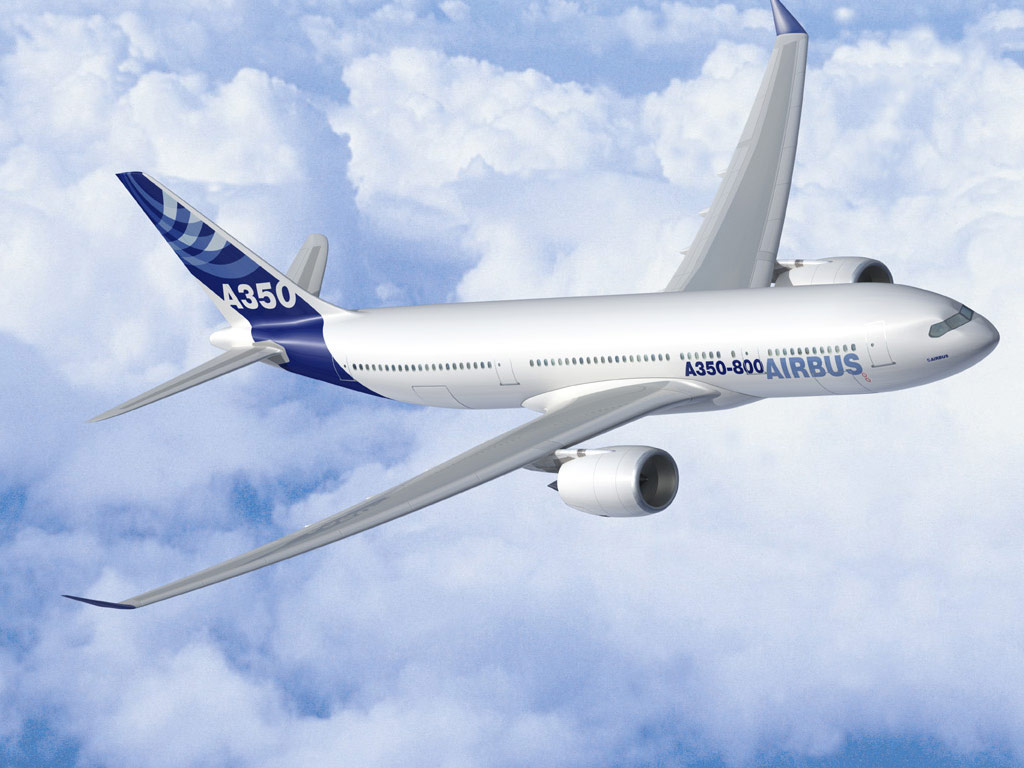
\includegraphics[height=50mm]{Figures/Airbus_A350.jpg}

% Title, author and degree
\vspace{0.8cm}
{\FontLb EagleEye} \\
\vspace{0.2cm}
{\FontMn Large photoset visualization } \\
\vspace{1.9cm}
{\FontMb Carlos Eduardo Henriques de Jesus Fonseca} \\
\vspace{1.9cm}
{\FontLn Disserta\c{c}\~{a}o para a obten\c{c}\~{a}o de Grau de Mestre em} \\
\vspace{0.3cm}
{\FontLb Engenharia Informática e de Computadores} \\
\vspace{1.9cm}
{\FontMb J\'{u}ri} \\
\vspace{0.3cm}
{\FontSn %
\begin{tabular}{ll}
Presidente: & Nome do Presidente \\
Orientador: & Nome do Orientador \\
Co-orientador: & Nome do Co-orientador \\
Vogais: & Nome do Vogal 1 \\
        & Nome do Vogal 2 \\
        & Nome do Vogal 3 \\
\end{tabular} } \\
\vspace{1.1cm}
{\FontMb M\^{e}s e Ano} \\
%
\end{center}

\cleardoublepage

 % file "Thesis_FrontCover.tex"

% ----------------------------------------------------------------------
% Dedication page (optional)
% ----------------------------------------------------------------------
%%%%%%%%%%%%%%%%%%%%%%%%%%%%%%%%%%%%%%%%%%%%%%%%%%%%%%%%%%%%%%%%%%%%%%%%
%                                                                      %
%     File: Thesis_Dedication.tex                                      %
%     Tex Master: Thesis.tex                                           %
%                                                                      %
%     Author: Andre C. Marta                                           %
%     Last modified : 21 Jan 2011                                      %
%                                                                      %
%%%%%%%%%%%%%%%%%%%%%%%%%%%%%%%%%%%%%%%%%%%%%%%%%%%%%%%%%%%%%%%%%%%%%%%%

\null\vskip5cm%
\begin{flushright}
     \red{Dedicated to someone special...}
\end{flushright}
\vfill\newpage

\cleardoublepage

 % file "Thesis_Dedication.tex"

% ----------------------------------------------------------------------
%  Acknowledgments (optional)
% ----------------------------------------------------------------------
%%%%%%%%%%%%%%%%%%%%%%%%%%%%%%%%%%%%%%%%%%%%%%%%%%%%%%%%%%%%%%%%%%%%%%%%
%                                                                      %
%     File: Thesis_Acknowledgments.tex                                 %
%     Tex Master: Thesis.tex                                           %
%                                                                      %
%     Author: Andre C. Marta                                           %
%     Last modified : 21 Jan 2011                                      %
%                                                                      %
%%%%%%%%%%%%%%%%%%%%%%%%%%%%%%%%%%%%%%%%%%%%%%%%%%%%%%%%%%%%%%%%%%%%%%%%

\section*{\acknowledgments}

% Add entry in the table of contents as section
\addcontentsline{toc}{section}{\acknowledgments}

\red{A few words about the university, financial support, research advisor, dissertation readers, faculty or other professors, lab mates, other friends and family...
}

\cleardoublepage

 % file "Thesis_Acknowledgements.tex"

% ----------------------------------------------------------------------
%  Abstract (both in English and Portuguese)
% ----------------------------------------------------------------------
%%%%%%%%%%%%%%%%%%%%%%%%%%%%%%%%%%%%%%%%%%%%%%%%%%%%%%%%%%%%%%%%%%%%%%%%
%                                                                      %
%     File: Thesis_Resumo.tex                                          %
%     Tex Master: Thesis.tex                                           %
%                                                                      %
%     Author: Andre C. Marta                                           %
%     Last modified : 21 Jan 2011                                      %
%                                                                      %
%%%%%%%%%%%%%%%%%%%%%%%%%%%%%%%%%%%%%%%%%%%%%%%%%%%%%%%%%%%%%%%%%%%%%%%%

\chapter*{Resumo e palavras chave}

% Add entry in the table of contents as section
\addcontentsline{toc}{section}{Resumo e palavras chave}

A fotografia digital tem feito parte da vida das pessoas na ultima década, crescendo nos discos rígidos, mas a visualização de imagens não tem vindo a evoluir o suficiente para acompanhar este crescimento. A maior parte das pessoas guarda as fotos em pastas ou utiliza programas que não conseguem mostrar grandes quantidades de fotografias ao mesmo tempo, não fornecendo uma visão global da biblioteca.

Este trabalho cresceu das características de outros trabalhos de visualizações alternativas de imagens e tenta trazer a utilizadores comuns uma melhor maneira de explorar as suas bibliotecas de fotografias e aprender mais sobre elas.

Este trabalho fornece um sistema extensível para a extracção e agregação de características das imagens do utilizador e respectivos meta-dados, Actualmente são extraidas cores, rostos, datas, pastas e palavras-chave, mas, já que é extensível, poderá ser utilizado para muito mais.

Também criámos uma aplicação de visualização que usa os dados processados e os disponibiliza aos utilizadores numa interface limpa e simples. A aplicação começa por apresentar no ecrã, numa grelha, todas as imagens adicionadas ao programa, agrupados por datas. A partir daqui, o utilizador pode alterar a visualização ampliando-a ou reduzindo-a, organizando as imagens por cores, rostos ou pastas, podendo ainda filtrar utilizando uma mistura de todos os dados recolhidos pelo sistema de processamento. Desta forma, os utilizadores podem visualizar e explorar suas bibliotecas de uma forma diferente daquilo a que estão habituados.

\vfill

\textbf{Palavras-chave:} fotografias, visualização de imagens, exploração de imagens, extração de caracteristicas

\cleardoublepage

 % file "Thesis_Resumo.tex"
%%%%%%%%%%%%%%%%%%%%%%%%%%%%%%%%%%%%%%%%%%%%%%%%%%%%%%%%%%%%%%%%%%%%%%%%
%                                                                      %
%     File: Thesis_Abstract.tex                                        %
%     Tex Master: Thesis.tex                                           %
%                                                                      %
%     Author: Andre C. Marta                                           %
%     Last modified : 21 Jan 2011                                      %
%                                                                      %
%%%%%%%%%%%%%%%%%%%%%%%%%%%%%%%%%%%%%%%%%%%%%%%%%%%%%%%%%%%%%%%%%%%%%%%%

\chapter*{Abstract and keywords}

% Add entry in the table of contents as section
\addcontentsline{toc}{section}{Abstract and keywords}

\red{Insert your abstract here with a maximum of 250 words, followed by 4 to 6 keywords...
}
\vfill

\textbf{Keywords:} \red{photographs, image visualization, image browsing},...

\cleardoublepage

 % file "Thesis_Abstract.tex"

% ----------------------------------------------------------------------
%  Table of contents, list of tables, list of figures and nomenclature
% ----------------------------------------------------------------------

% Table of contents
%
\tableofcontents
\cleardoublepage 

% List of tables
%
% Generate list
\listoftables
% Add entry in the table of contents as section
\addcontentsline{toc}{section}{\listtablename}
\cleardoublepage 

% List of figures
%
% Generate list
\listoffigures
% Add entry in the table of contents as section
\addcontentsline{toc}{section}{\listfigurename}
\cleardoublepage 

%%%%%%%%%%%%%%%%%%%%%%%%%%%%%%%%%%%%%%%%%%%%%%%%%%%%%%%%%%%%%%%%%%%%%%%%
%                                                                      %
%     File: Thesis_Nomenclature.tex                                    %
%     Tex Master: Thesis.tex                                           %
%                                                                      %
%     Author: Andre C. Marta                                           %
%     Last modified : 21 Jan 2011                                      %
%                                                                      %
%%%%%%%%%%%%%%%%%%%%%%%%%%%%%%%%%%%%%%%%%%%%%%%%%%%%%%%%%%%%%%%%%%%%%%%%
%
% The definitions can be placed anywhere in the document body
% and their order is sorted by <symbol> automatically when
% calling makeindex in the makefile
%
% The \glossary command has the following syntax:
%
% \glossary{entry}
%
% The \nomenclature command has the following syntax:
%
% \nomenclature[<prefix>]{<symbol>}{<description>}
%
% where <prefix> is used for fine tuning the sort order,
% <symbol> is the symbol to be described, and <description> is
% the actual description.

% ----------------------------------------------------------------------

\chapter*{Acronyms}

% Add entry in the table of contents as section
\addcontentsline{toc}{section}{Acronyms}

\begin{acronym}[TDMA]

\acro{UI}[UI]{user interface}
\acro{UX}[UX]{user experience}
\acro{SOM}[SOM]{self organizing map}
\acro{CBIR}[CBIR]{content based image retrieval}
\acro{MP}[MP]{megapixel}
\acro{FEP}[FEP]{feature extraction plugin}
\acro{WPF}[WPF]{Windows Presentation Foundation}
\acro{EXIF}[EXIF]{Exchangeable image file format}
\acro{HDR}[HDR]{High Dynamic Range}

\end{acronym}
\vfill

\cleardoublepage % file "Thesis_Nomenclature.tex"

%
% Insert glossary/nomenclature section produced by MakeIndex
%\printnomenclature
% Add entry in the table of contents as section
%\addcontentsline{toc}{section}{\nomname}
\cleardoublepage

% Set arabic numbering (1,2,...) after preface
%

\setcounter{page}{1}
\pagenumbering{arabic}

% ----------------------------------------------------------------------
%  Chapters
% ----------------------------------------------------------------------


\chapter{Introduction} % 5/6 pages
\label{chapter:introduction}


% \section{Prologue} % (fold)
% \label{sec:prologue}

\setlength{\epigraphwidth}{.5\textwidth}
\setlength{\afterepigraphskip}{\baselineskip}

\epigraph{\emph{\textbf{photography}}\newline
noun\newline
the art or practice of taking and processing photographs.}{\footnotesize New Oxford American Dictionary 3rd edition}

Photography is a very personal activity. Each person has its own way of doing it, with its own devices, software and techniques. It ranges from common people who take photos of their cats using their low quality camera phones to put on the internet, up to professional photographers with big cameras and lenses to take award-winning photos and everything in between. Digital cameras have brought photography to the masses with its ease of use, no cost per photo and easy processing made photography skyrocket. Flickr\footnote{\url{http://flickr.com} is, probably, the most used photo-sharing website worldwide.} has reached the 6.000.000.000 upload in August 2011 and seeing a 20\% increase year-over-year since the website's debut in 2004\footnote{According to a blog post on the Flickr website \url{http://blog.flickr.net/en/2011/08/04/6000000000}}.

Not only are people taking more and more photos but some photography techniques that use multiple photo captures also appeared or, at least, became more relevant with the digital cameras among some enthusiasts and professional photographers, like burst photographs, where many photos are taken in a quick sequence to capture a motion sequence, or panoramas that are made from various overlapping photos of a subject that is bigger then what the camera can capture or even something called \acf{HDR} photography that merges multiple captures to correct the lack of capacity of the sensors to capture very dark and very bright areas on the same scene.

This growth of the digital brings the problem that photo collections have started to grow more than they used to, in the film era. But storing digital photographs isn't that different from the past. In fact, people have been storing their photographs on folders on their computers instead of photo albums on the shelf. One could say computers can help people view, explore and find more photos in a shorter period of time, they certainly have the power for that but, in the end, they usually don't do much more than make the user look for the photo album (probably a folder or an ``album'' on some applications) and then flick through its pages (scrolling) until the photos the user was looking for appear.

This is true for the most common photo management software on the market, like Google's Picasa\footnote{\url{http://picasa.google.com}}, Apple's iPhoto\footnote{\url{http://www.apple.com/iphoto}} or Aperture \footnote{\url{http://www.apple.com/aperture}}, or Adobe's Lightroom \footnote{\url{http://www.adobe.com/lightroom}}. Although they bring some management improvements with them, the analogy above still applies. They all provide a way to select albums or folders and scroll through contents. They allow searching through some existing metadata, the only metadata that some of them generate is only face detection and end up having lots of buttons, toggles and options for their editing capabilities that clutter the interface. All of this, added to the fact that collections quickly reach the thousands of images, prohibit a global view of the collection. It's not easy to gather all the images that are spread across the system and view them all together, understanding its evolution and characteristics.

\section{Our vision} % (fold)
\label{ssub:our_vision}

% subsubsection our_vision (end)

We want to provide the users a totally different way to visualize their photos by focusing only on them. We want to give them an birds-eye view of their photos by showing everything and allowing them to drill down and view any image they want at a large size. We want users to see their collections in new ways, and try to understand, e.g., how their photography has evolved over time.

With this work we will show that this dynamic visualization is a much better exploration tool than other, more common, software applications.

\todo{expand}


% section prologue (end)


\section{Contributions} % (fold)
\label{sec:contributions}

With our work, we have understood that visualization of large collections at the same time is not only feasible but also interesting to the users. 

We observed that images can be really small and still be identifiable by their owners, as long as they are integrated with others of the same event.

\todo{moar stuff here}

% section context (end)


\section{Structure of the Document} % (fold)
\label{ssub:structure_of_the_document}

We will start by going through some previous work related to ours (chapter \ref{chapter:related-work}) followed by an identification of the requirements for our work (chapter \ref{chapter:solution_requirements}). Next, we will see what was implemented and how it works (chapter \ref{cha:eagle_eye}) and how the users responded to it (chapter \ref{chapter:evaluation}). To conclude, we will discuss some work that could be done to improve this thesis (chapter \ref{future_work}) and final thoughts to conclude (chapter \ref{chapter:conclusions}).

% subsubsection structure_of_the_document (end)


\chapter{Related Work}
\label{chapter:related-work}

% Should be around 20 pages

Interactive image visualization techniques have been explored for some time now, many of them related to image organization or retrieval in large collections. There have been some interesting ideas across the board and we will now take a look at some of them.


\section{Related work}

\subsection{Visual guided navigation for image retrieval} % (fold)
\label{sub:Qiu}

Qiu et al. \cite{Qiu:2007p1207} explore the requirements of a system intended for visualizing large photo collections. They identify as the two most important requirements, the first being an easy to use \ac{UI}, that gives clean information to the user and helps to create a mental image of the whole collection helping him to navigate on the collection. The second requirement is responsiveness because while image processing can be an heavy task, the user needs to be able to interact with the interface and he won't use the application if it's slow. 

\begin{figure}[ht]
	\centering
		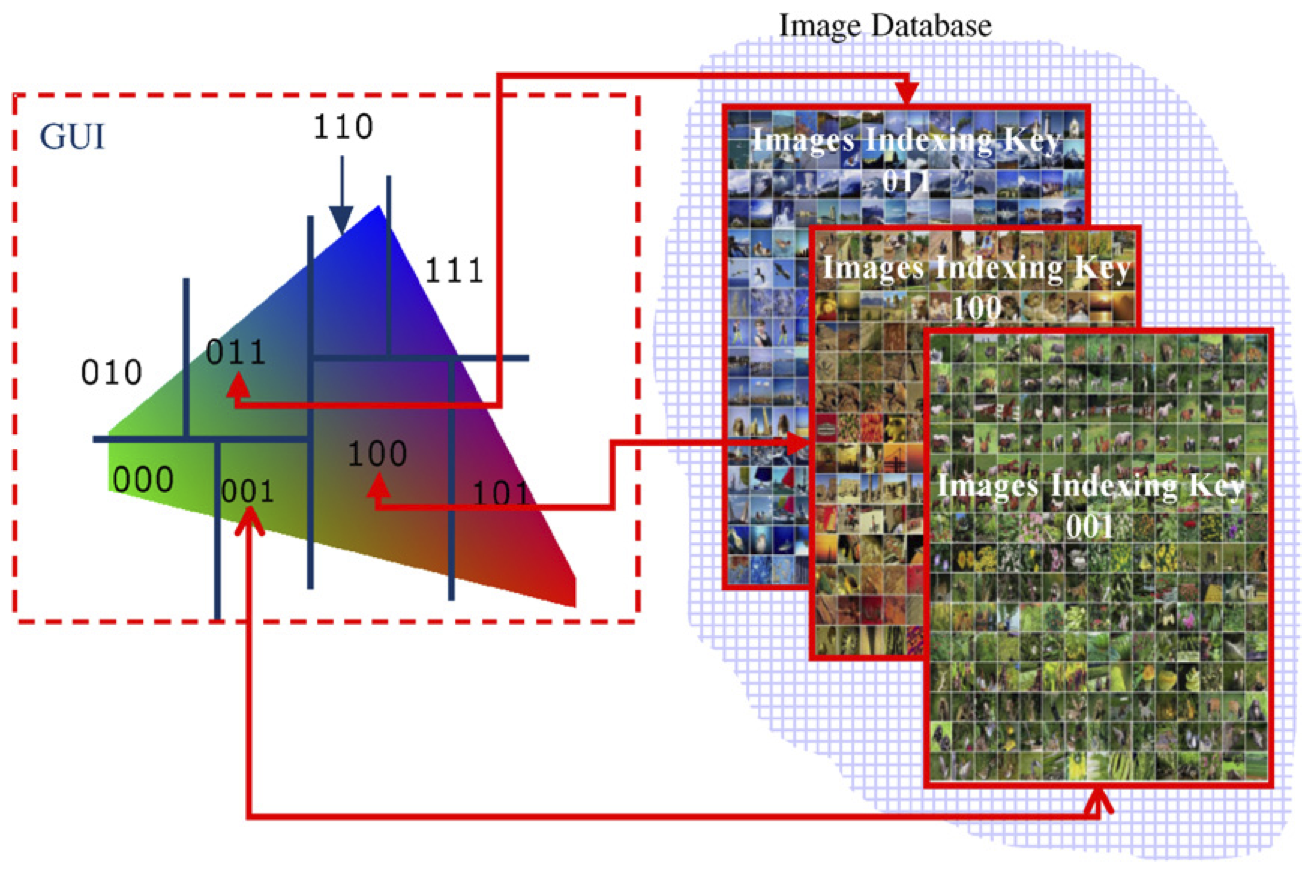
\includegraphics[width=0.6\columnwidth]{imgs-RelatedWork/Qiu-2007p1207.png}
	\caption[Chromacy diagram and color related images, from the work of Qiu et al.]{The chromacy diagram is split in parts and each image belongs to one of this parts. The diagram is part of the \ac{UI} and  when navigating through the diagram, only the images related to that part are shown.}
	\label{fig:qiu1}
\end{figure}

The system shows all the photos arranged by color, just as many others like it. The difference is the process in use. Instead of calculating distance vectors based on the histogram of each image, this approach classifies each image with a simple description, like an average of its colors, and arranges them by that value, on a color map (\fig{qiu1}). The process is much faster, but is also more error prone, specially on photos without a clear main color.

Their tests show they achieved good responsiveness and better results than using a file explorer.

% section Qiu (end)

\subsection{Does organization by similarity assist image browsing?} % (fold)
\label{sub:Rodden}
\begin{figure}[ht]
	\centering
		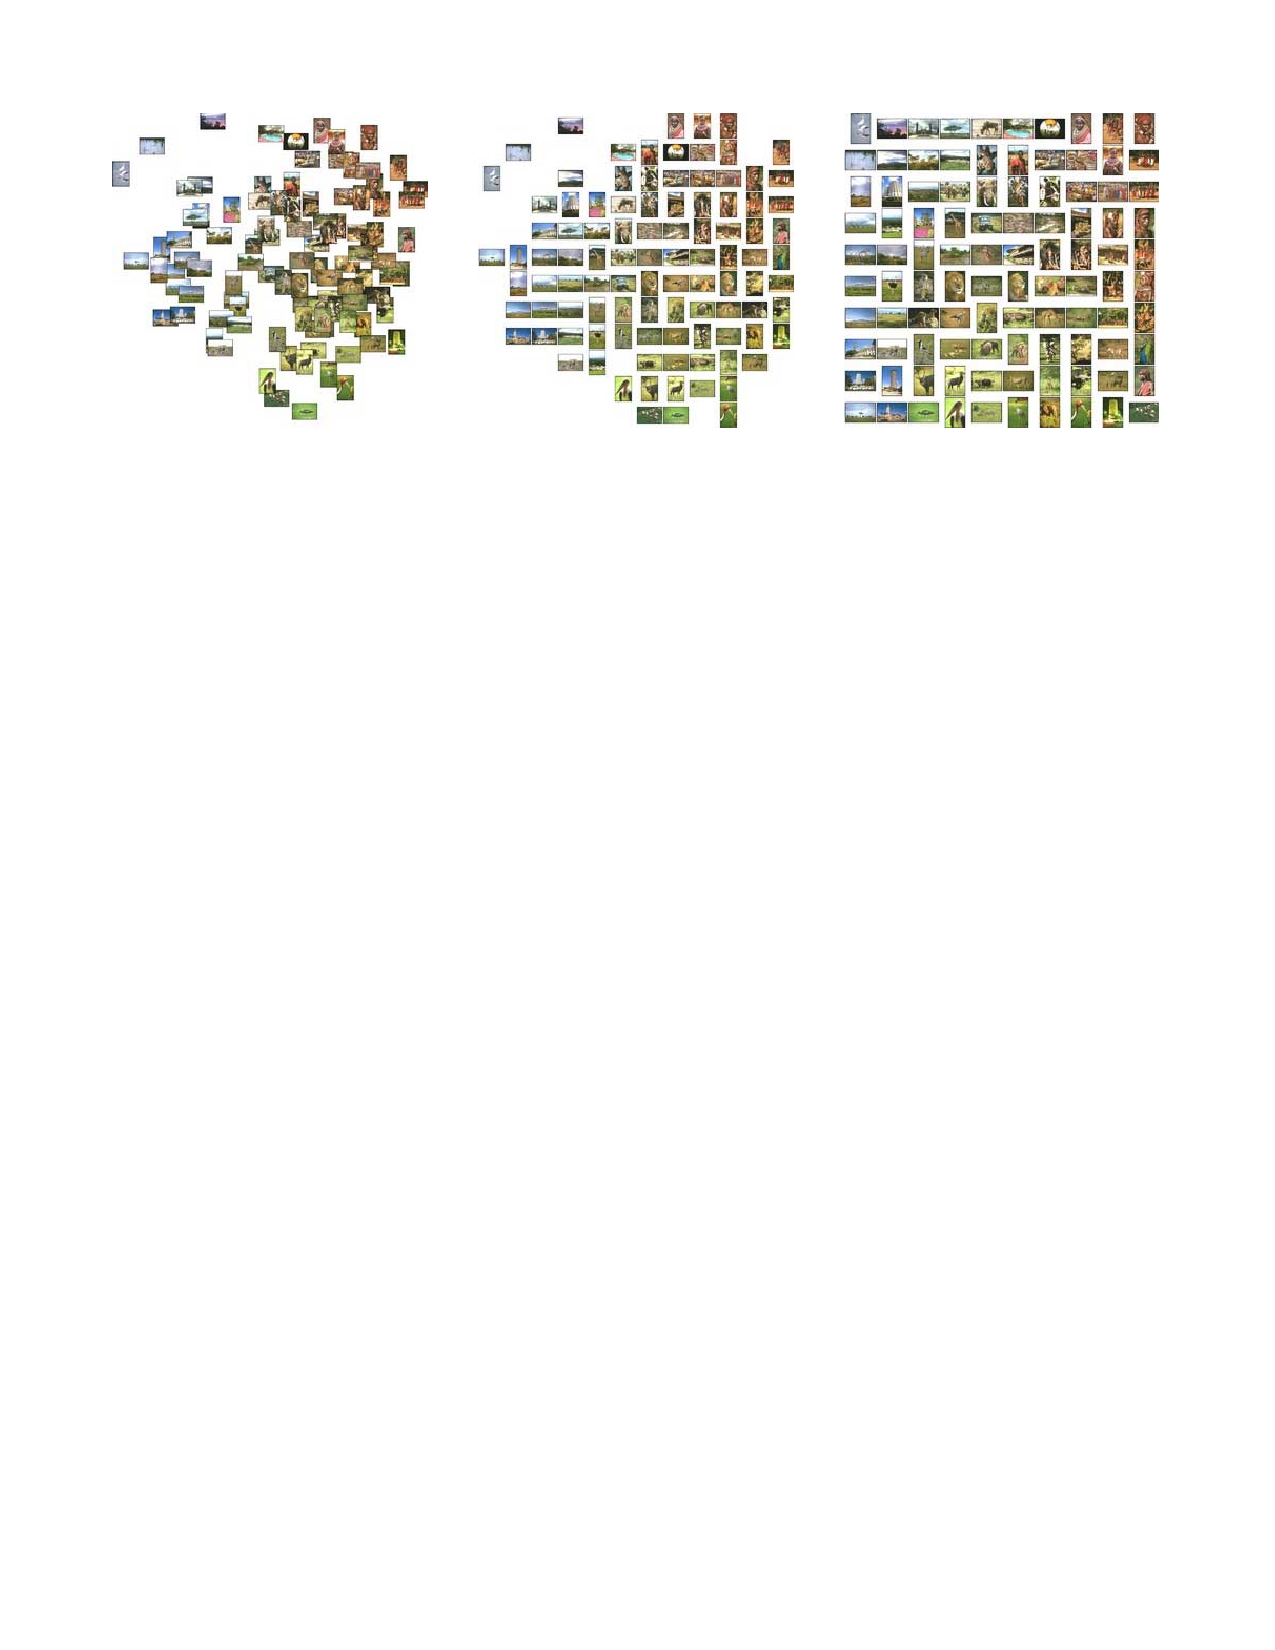
\includegraphics[width=\textwidth]{imgs-RelatedWork/Rodden1}
	\caption[Three arrangements of 100 images of Kenya, based on visual similarity, from the work of Rodden and Sinclar]{Three arrangements of 100 images of Kenya, based on visual similarity. On the left is the arrangement with overlap, in the middle a 12x12 grid (which removes the overlap while preserving some of the structure), and on the right a 10x10 grid (which maximises the thumbnail size).}
	\label{fig:Rodden1}
\end{figure}

The aim of this work by Rodden and Sinclar \cite{Rodden:2001p731} was to evaluate how photo organization by similarity (\fig{Rodden1}) could benefit a user looking for images. Some users tested an application that could show the same images both in a random and in an organized by similarity way. This organization by similarity was based on a rough description of the images, but it could be other descriptors.

The results differ if the user knows what he's looking for or not. In case he does, being able to filter only the relevant images makes it quick to find the ones that matter. This obviously depends on the quality of the labeling. Users reported that sometimes the similar images appear to merge.

In case the user doesn't know what he's looking for, the random approach might be helpful because the strong images usually contrast to their neighbors and thus appear to stand out.

For some people, having access to different arrangements of the same set of images is useful, although the source of the individual differences still needs to be determined.

% section Rodden (end)


\subsection{Browsing large collections of images through unconventional visualization techniques} % (fold)
\label{sub:Porta}

\begin{figure}[!htb]
  \begin{subfigmatrix}{2}
    \subfigure[Spot display]{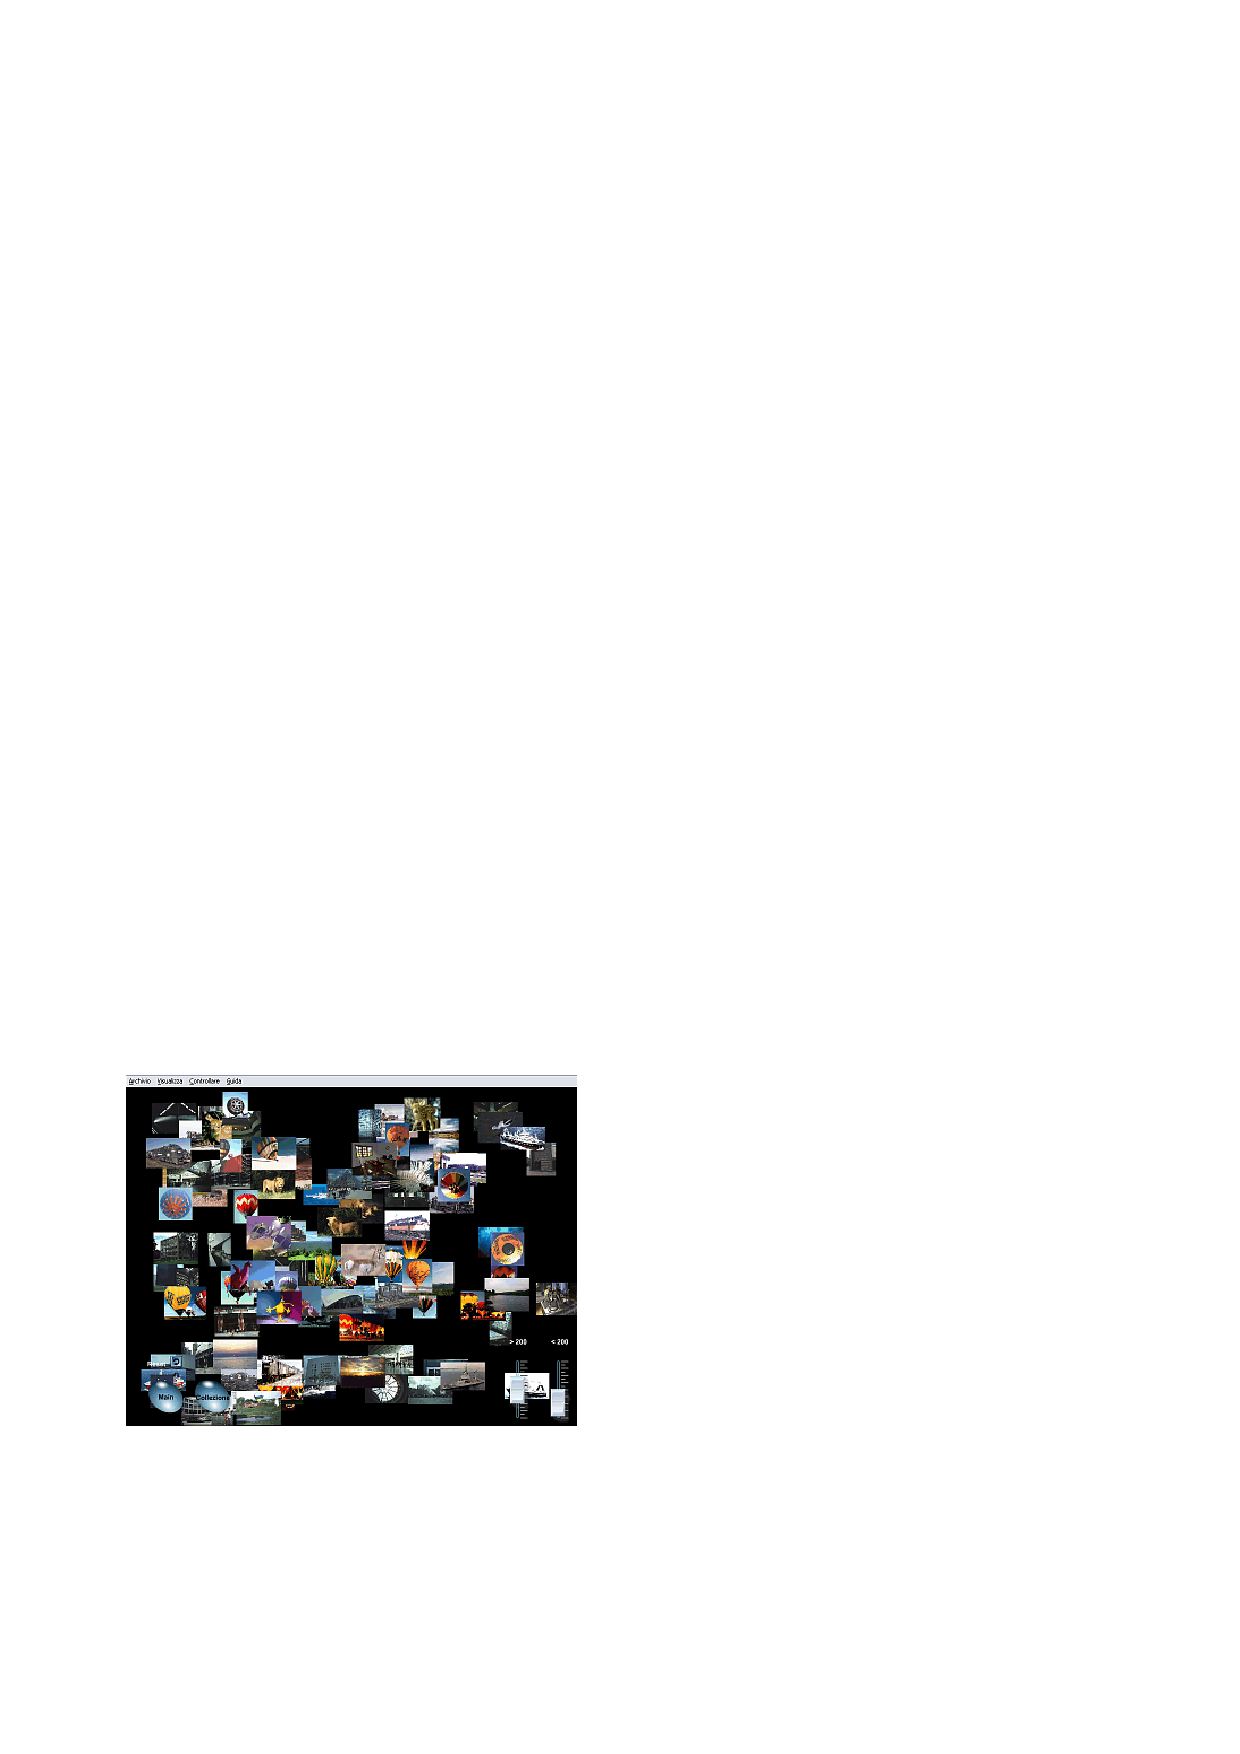
\includegraphics[width=0.49\linewidth]{imgs-RelatedWork/Porta-spot}\label{fig:porta-spot}}
    \subfigure[Shot display]{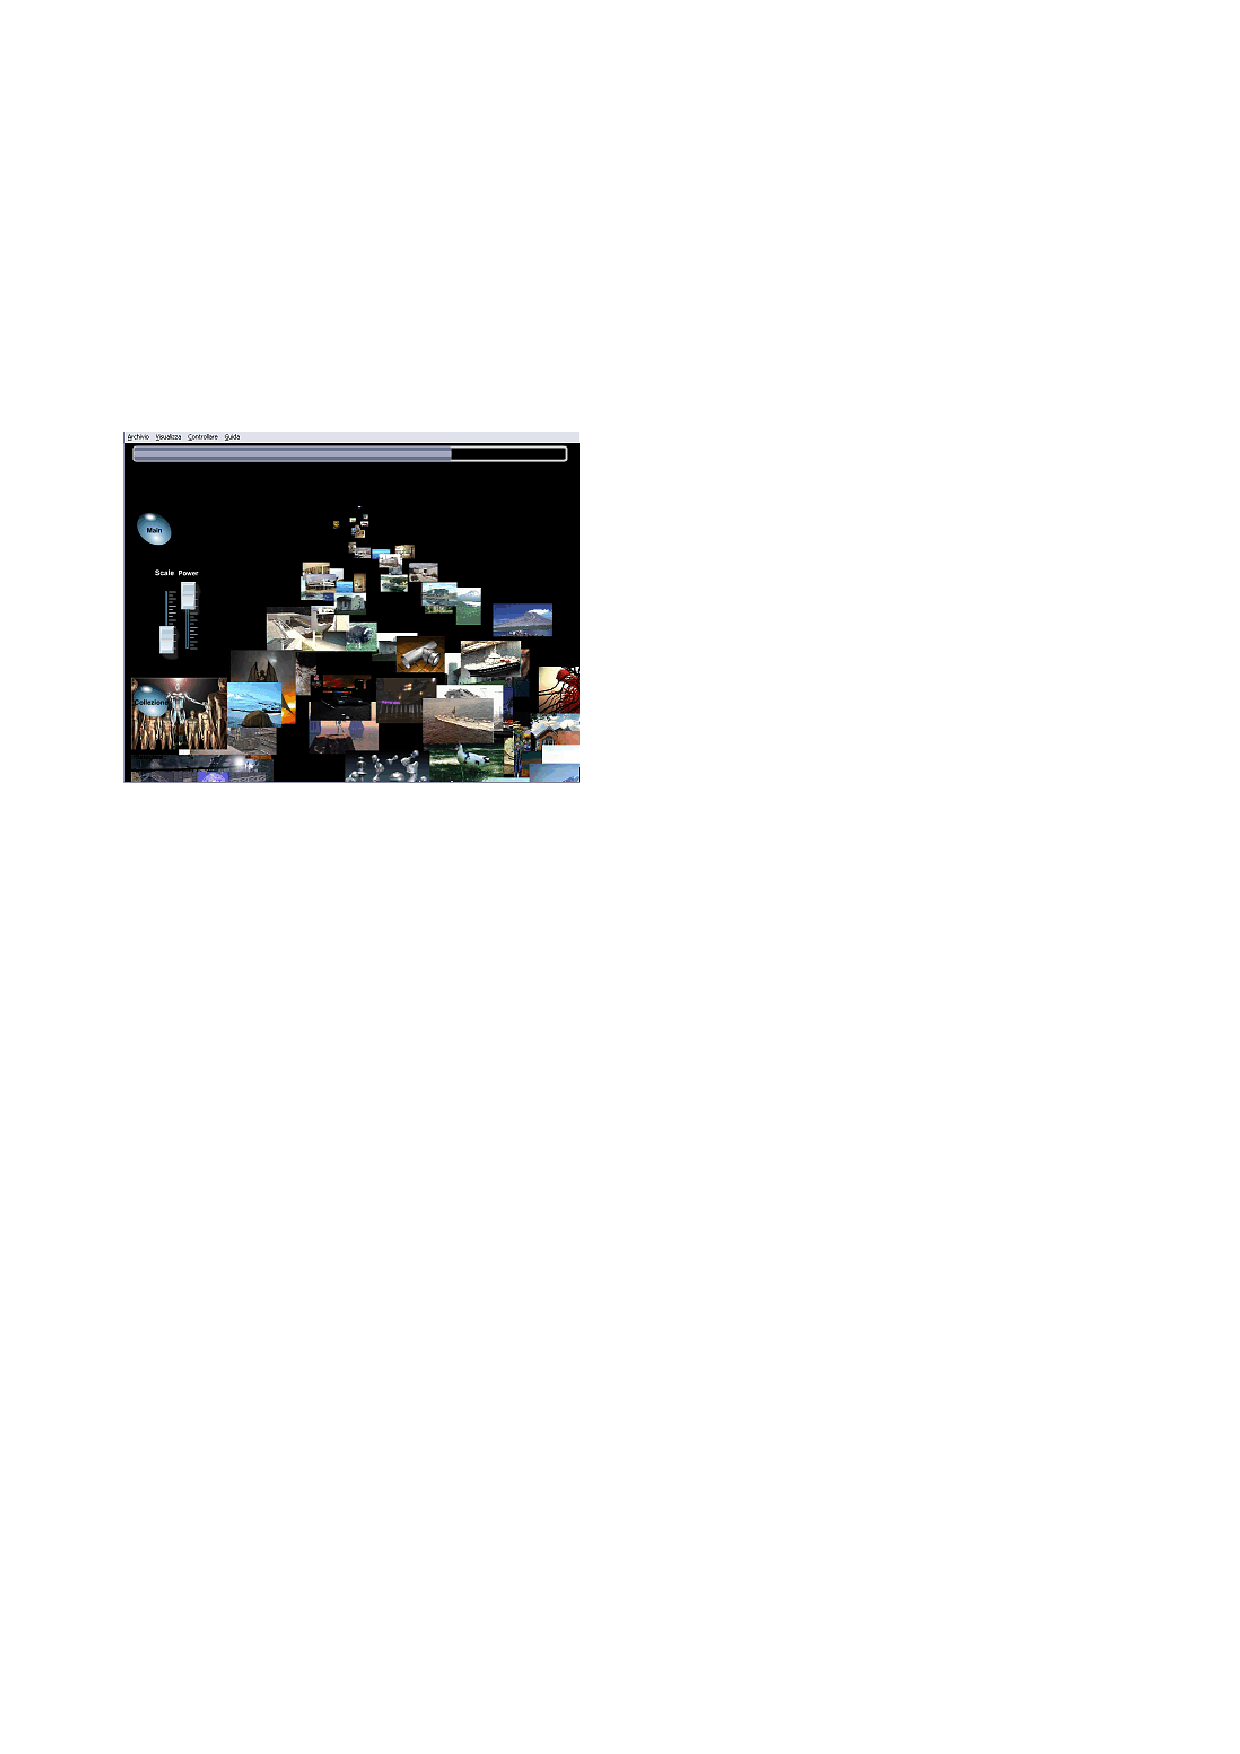
\includegraphics[width=0.49\linewidth]{imgs-RelatedWork/Porta-shot}\label{fig:porta-shot}}
  \end{subfigmatrix}
  \caption{The two better visualizations from Porta's work.}
  \label{fig:porta}
\end{figure}


Porta \cite{Porta:2006p416} describes a few visualization methods for large collections of images and tests them with users. The purpose is to find ways or metaphors that provide a good visualization experience in terms of time spent and quality of the visualization.

Some of the various techniques were the simple image grid view, a grid view with variable and independent height and width (EIB), a view that animates images like they were shot from a distance and get closer to the user called Shot (\fig{porta-shot}), a view where images quickly appear on random positions on screen named Spot (\fig{porta-spot}), and some other less commons like one that simulates a cylinder created with images (Cylinder), and others less relevant (Rotor, Tornado and Tornado of Planes).

The testing was based on the efficiency of users searching for specific images on a collection of a thousand photos. The Spot view was the best, followed the Shot, Cylinder finally the common grid view. The other views got scores near or below the grid view.

% section Porta (end)

\subsection{A comparison of static and moving presentation modes for image collections} % (fold)
\label{sub:Cooper}

This paper by Cooper et al. \cite{Cooper:2006p543} is not about large libraries, but about what kind of interfaces for image showing has greater success of user recognition and preference (\fig{Cooper1}).

With the help of eye-tracking techniques and user preference, the authors determined that static images are better than moving ones because makes them easier to recognize and avoid some user confusion.

\begin{figure}[ht]
	\centering
		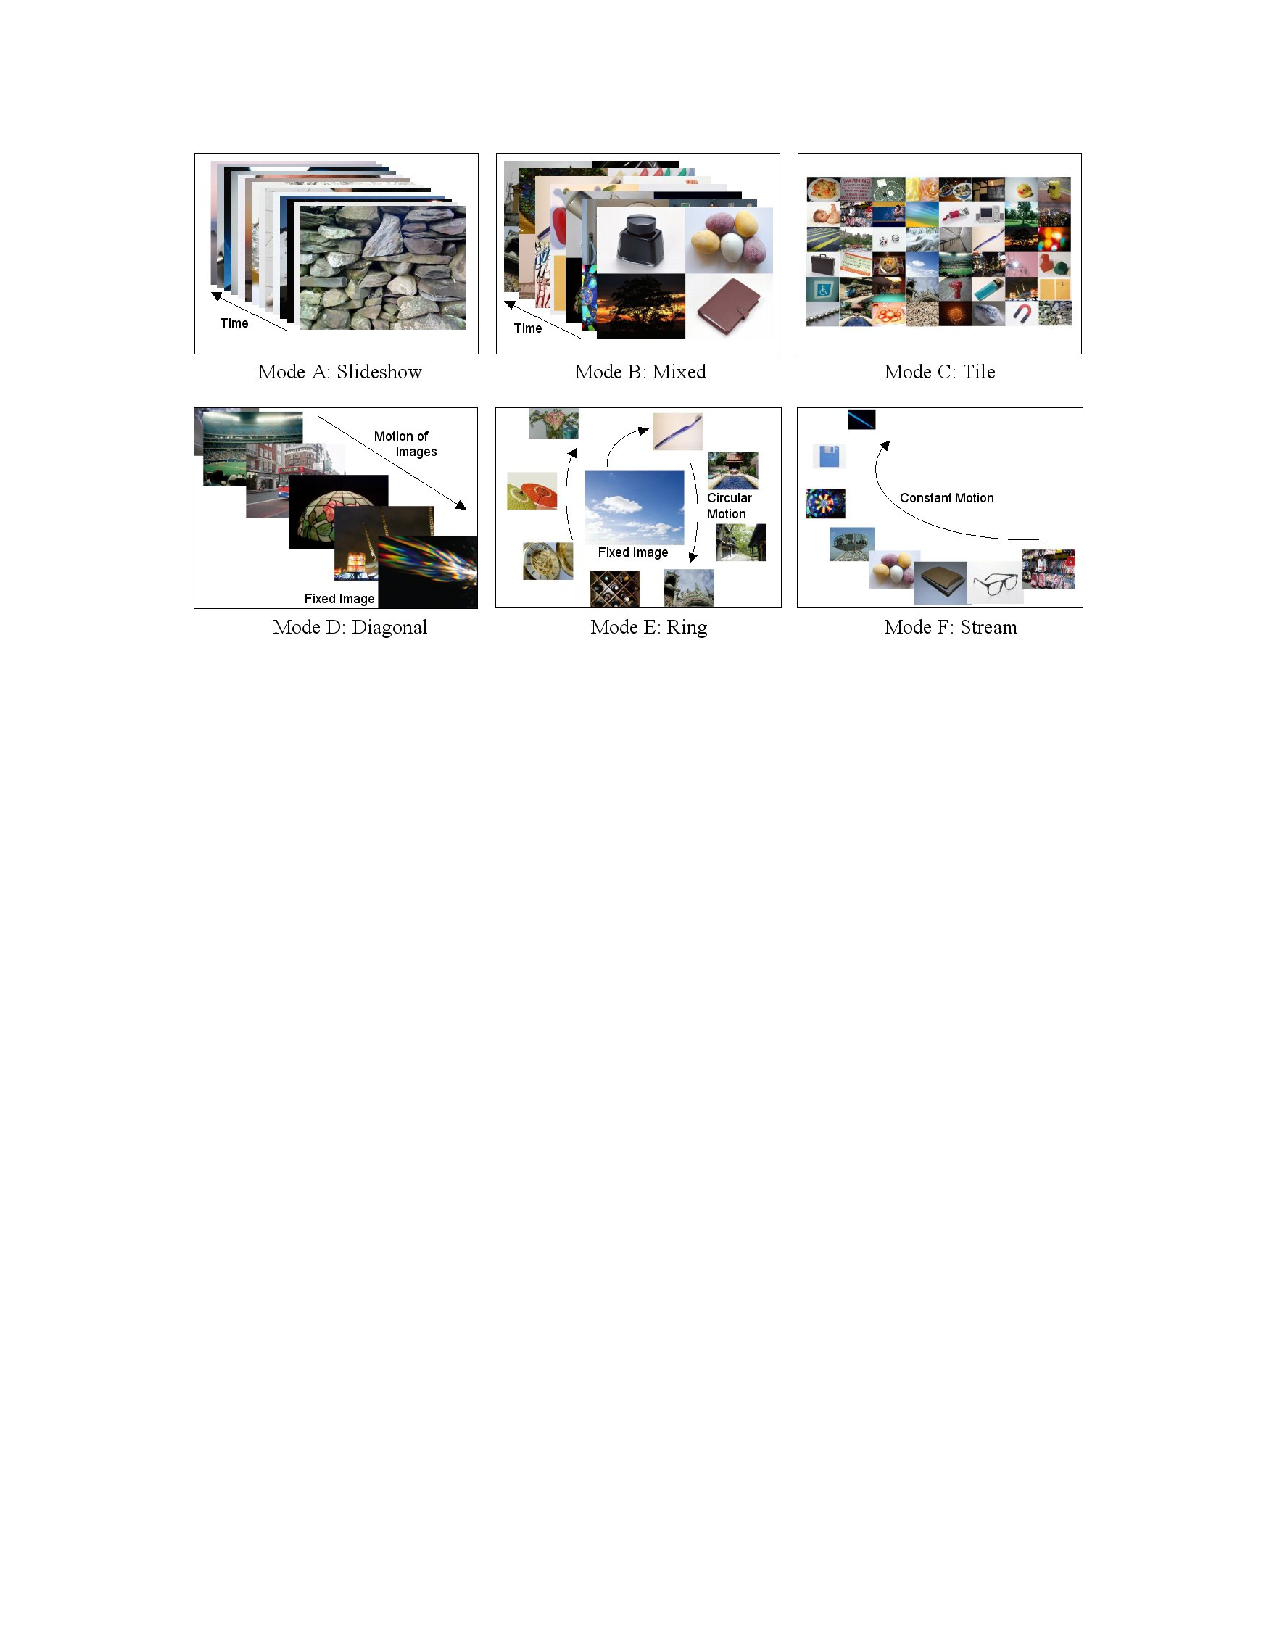
\includegraphics[width=\textwidth]{imgs-RelatedWork/Cooper1}
	\caption{The six rapid serial visual presentation modes used in the experiments}
	\label{fig:Cooper1}
\end{figure}
% section cooper (end)

\subsection{Organizing and browsing photos using different feature vectors and their evaluations} % (fold)
\label{sub:Strong}

Although it doesn't mention why, Strong \cite{Strong:2009p413} focuses on the better experience provided by color organization of a large image collection (\fig{Strong1}).

A \ac{SOM} is used to display the images on the screen featuring zooming, panning and sorting capabilities. The work is then based around the various methods used to determine the images' similarity.

Simpler methods are based on color histograms, which aren't affected by rotations or scales but, by not having spacial information on colors, allows very different images be closer together.

Other methods rely on gradients which contain spatial information and, therefore, are sensitive to image contents, but not color.
In general, the best methods were found to be the hybrid ones, where both color histograms and gradients are used to classify the images.
No user testing is made in this project, neither is the speed of image categorization referred about the methods used.

\begin{figure}[ht]
	\centering
		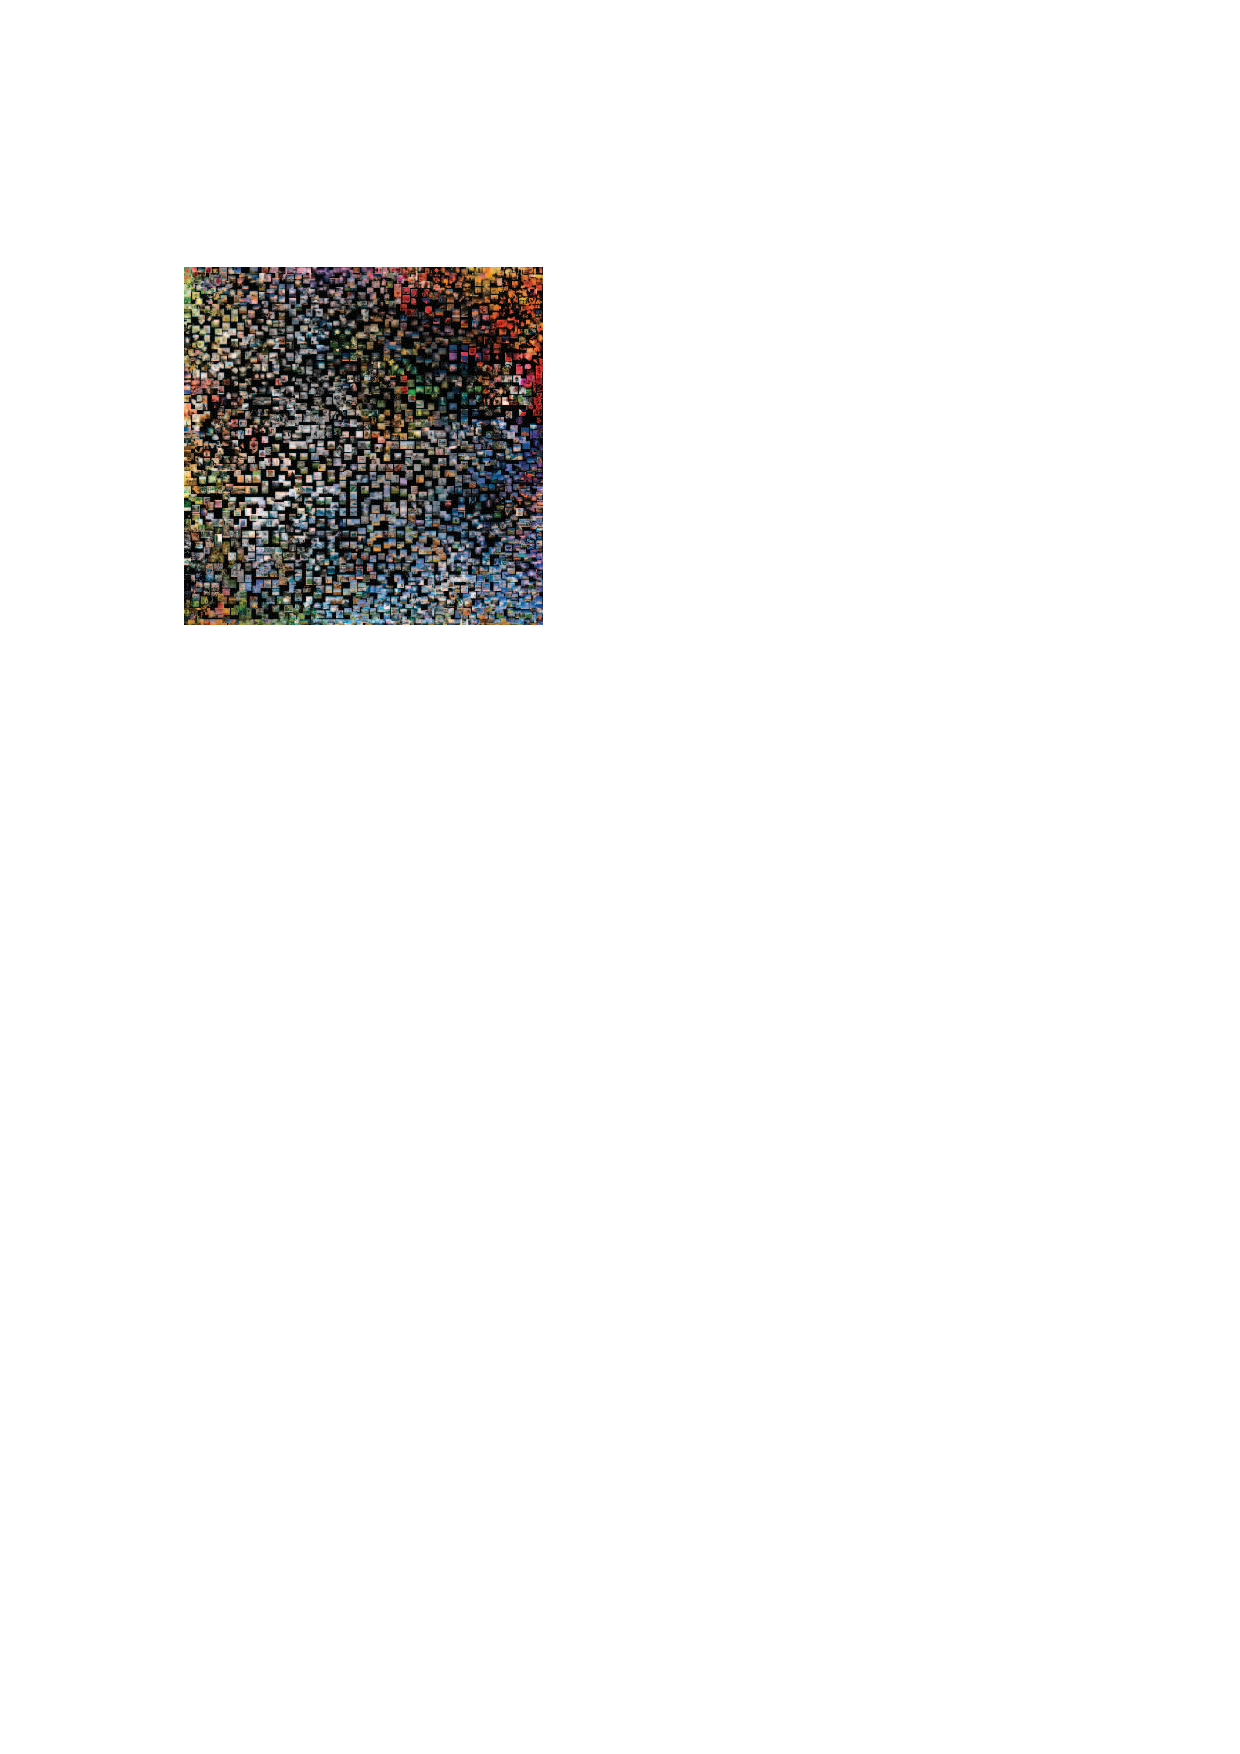
\includegraphics[scale=1]{imgs-RelatedWork/Strong1}
	\caption{The result obtained for organizing 2200+ photos using color autocorrelogram feature vector, using Strong's work \cite{Strong:2009p413}.}
	\label{fig:Strong1}
\end{figure}

% section strong (end)

\newpage
\subsection{An evaluation of color-spatial retrieval techniques for large image databases} % (fold)
\label{sub:Tan}
% não tem imagens

Tan et al. \cite{Tan:2001p850} present an evaluation of three color-spatial image retrieval techniques.

The signature-based technique creates a signature for each image, based on the most frequent colors, according to a threshold, of each subdivision, or bin, of that image. The comparison between images is made by comparing the main colors present on each bin. It is possible to assign more weight to specific bins according to the user's interest.

The partition-based approach is also based on bins, each having it's own color histogram. The similarity between images is given by the distance of the histograms of the corresponding bins.

The cluster-based method bases on the fact that humans focus on large patches (clusters) of the same color and, therefore, two images will appear similar if both have similar colored clusters on at roughly the same location. This method extracts the larger clusters and their color from each image. The similarity is calculated by the amount of overlap between clusters.

This techniques were tested with a collection of 12,000 images and, besides the color information, the brightness was also analyzed for increased performance. The authors conclude the signature method was generally better on both effectiveness and efficiency.

% section tan (end)

\subsection{Automatic organization for digital photographs with geographic coordinates} % (fold)
\label{sub:Naaman}

In this paper, by Naaman et al. \cite{Naaman:2004p1802}, is described a system that organizes digital photographs accordingly to location and date embedded on the metadata.

The objective was trying to mimmic the way people think about their collections. Photos are usually bursts separated by some time. Based on this and on the different places, events can be created to agglomerate photos from the same bursts. Location naming is done by calculating the most relevant places, like parks or cities, and then mixing the more precise locations with the more important neighbor cities to create a relevant and identifiable name. This was specially important since this work didn't involve showing any maps, but only the location names and events.

The authors showed good results and, nowadays, some common applications use similar features although including maps.
% section naaman (end)

\subsection{Similarity pyramids for browsing and organization of large image databases} % (fold)
\label{sub:Chen}

Chen et al. \cite{Chen:1998p2344} present a method for designing a hierarchical browsing environment called a similarity pyramid. The similarity pyramid groups similar images together while allowing users to view the database at varying levels of resolution. Each level is organized such that similar images are in close proximity on a two-dimensional grid (\fig{Chen1}). Images are first organized into a binary tree through agglomerative clustering based on color, edge and texture similarities. The binary tree is transformed into a quadtree, a tree in which each node has four children instead of only two.

\begin{figure}[ht]
	\centering
		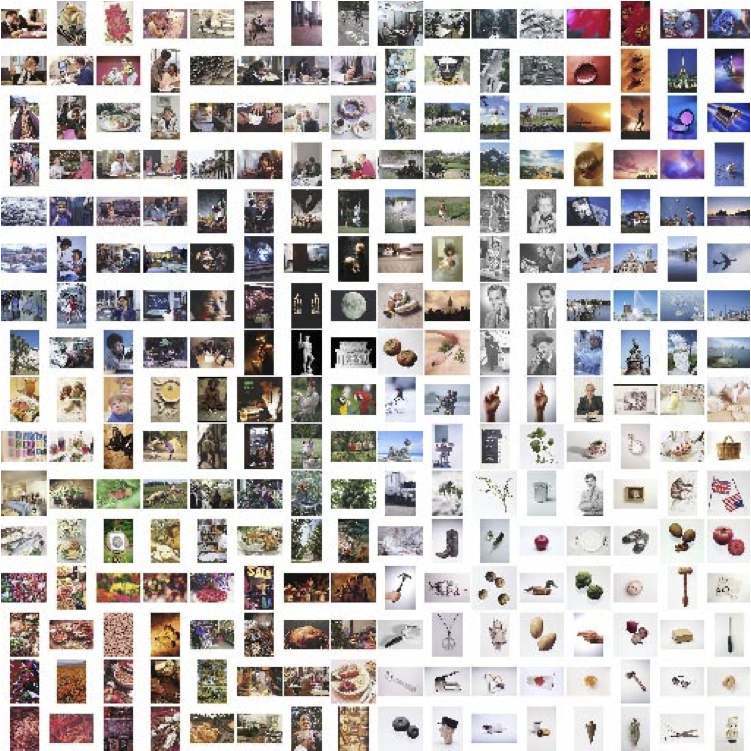
\includegraphics[scale=0.8]{imgs-RelatedWork/Chen-1998p2344.png}
	\caption{Images organized with \cite{Chen:1998p2344}. Images with similar color and texture are spatially adjacent.}
	\label{fig:Chen1}
\end{figure}

The similarity pyramid is best constructed using agglomerative (bottom-up) clustering methods, and a fast-sparse clustering method is presented which dramatically reduces both memory and computation over conventional methods. This method is based on the flexible agglomerative clustering algorithm, but using only a sparse proximity matrix and exploiting the author's approximate branch and bound search algorithm.

The authors found that the method for mapping the clustering to a pyramid can make a substantial difference in the quality of organization. Finally, a dispersion metric for objectively measuring pyramid organization was proposed, and found that it correlated well with the author's subjective evaluations of pyramid organization.

% section Chen (end)


\subsection{NN\super{k} networks for content-based image retrieval} % (fold)
\label{sub:Heesch}

Heesch \cite{Heesch:2004p2675} describes a different interaction technique for content based search in large image collections. Each image is a vertex in a graph and arcs are established between images if there exists at least one combination of features for which one image is retrieved as the nearest neighbor of the other. Each arc is weighted by the proportion of feature combinations for which the nearest neighbor relationship holds. By integrating the retrieval results over several feature combinations, the resulting network helps expose the semantic richness of images.

The interface reflects the vertexes and respective arcs, allowing to browse between the related images (\fig{heesch1}) in the network.

\begin{figure}[ht]
	\centering
		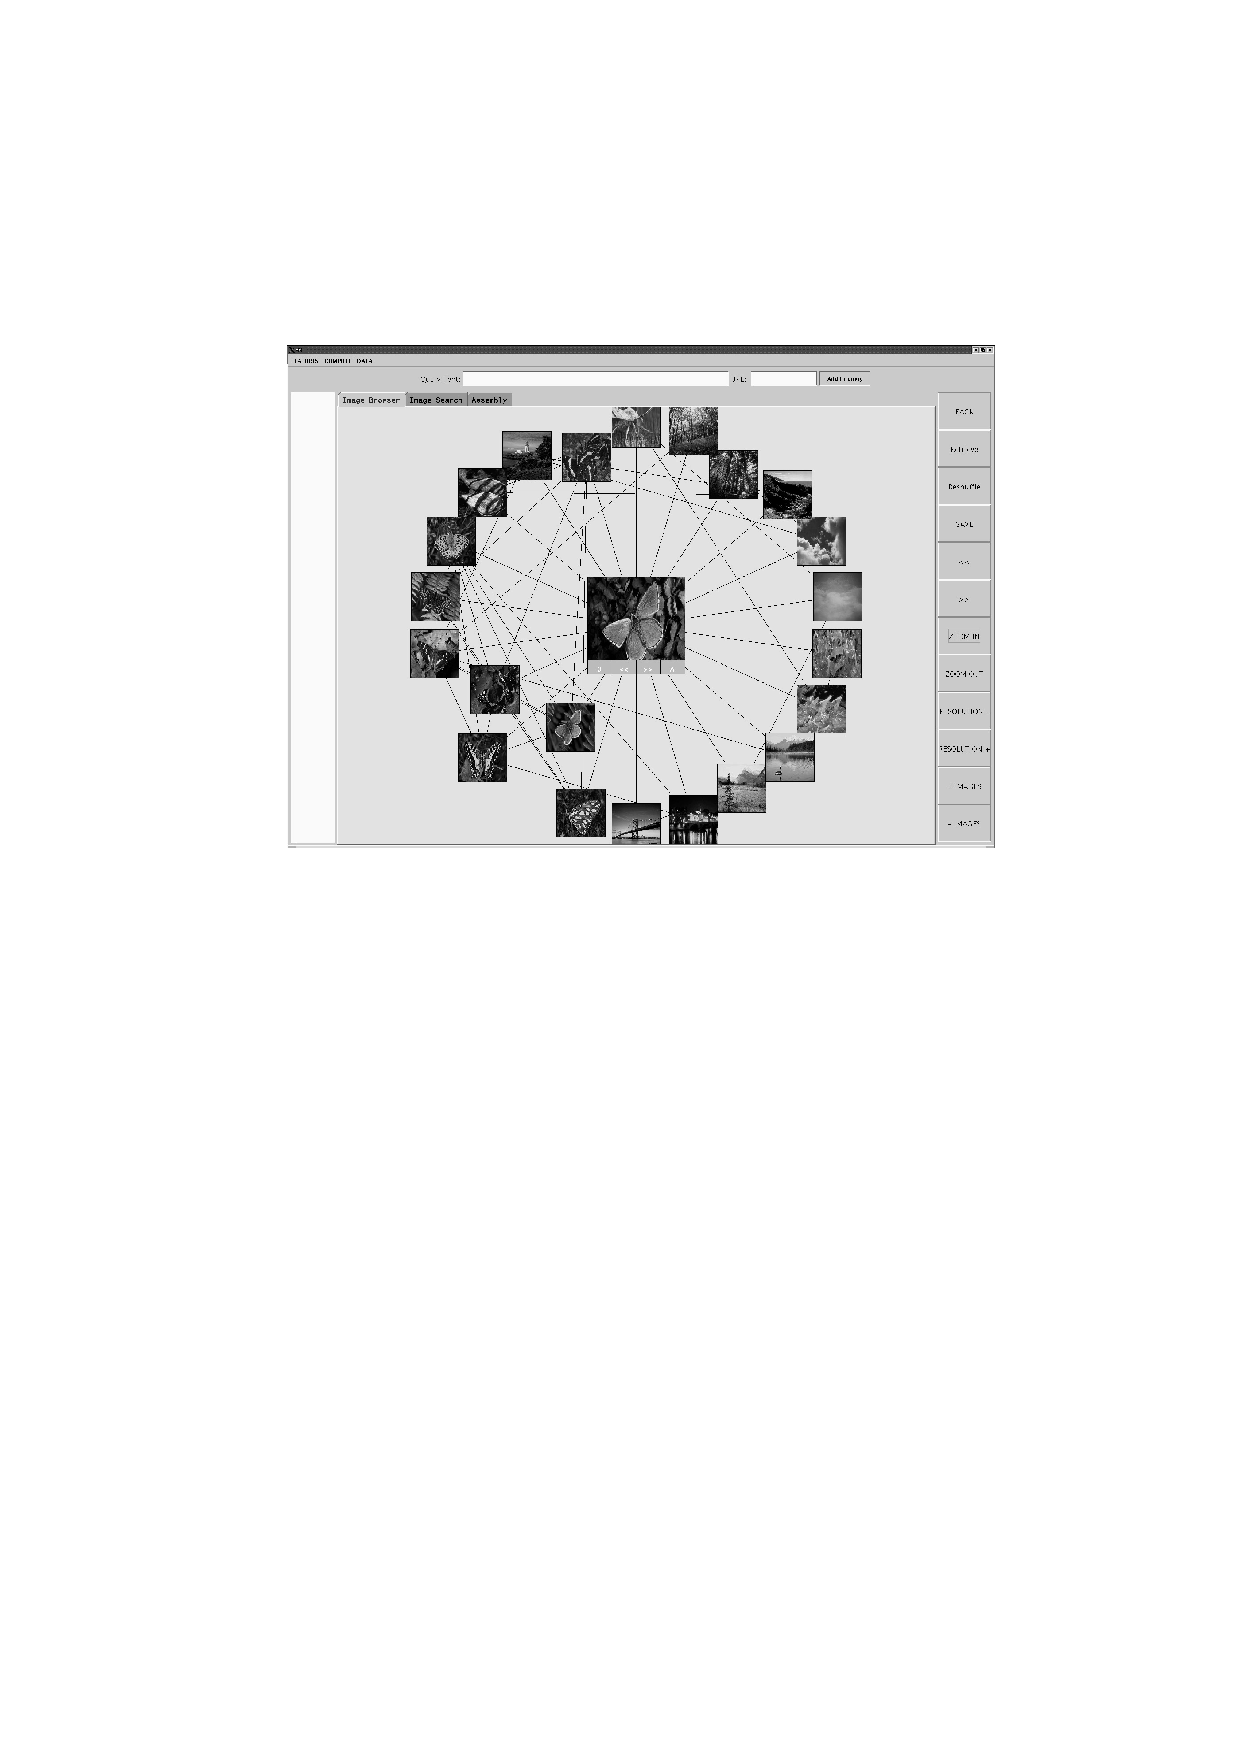
\includegraphics[scale=1]{imgs-RelatedWork/Heesch-2004p2675}
	\caption{Local network around the chosen butterfly image depicted in the middle.}
	\label{fig:heesch1}
\end{figure}

Seven low-level features are used for the classification of the images. HSV Global color Histograms maps the images by color, saturation and brightness; color Structure Descriptor maps the distribution of colors by dividing each image in 64 windows, the color space in 184 bins and associating color bins with image windows; Thumbnail feature compares identical images by saving the grey value of each pixel from a scaled down version of the image; Convolution filters discovers very selective features by reapplying 25 filters three times; Variance feature calculates standard deviations within a sliding window; Uniformity Feature is another statistical feature, calculating the grey level of an image split in 64 parts; Bag of words is the last feature and weights words associated to each image.

Tests showed great results when using a mix of search, relevance feedback and browsing, and even browsing by itself was considerably better than other, more restrictive, approaches.

The technique helps avoid the problem of image polysemy by showing all gathered meanings of the images to the user.
The feature network is pre-computed, allowing for quick realtime browsing. The authors claim it took 50 hours to process 32000 images, but made no reference to the possibility adding images to the collection, after the computation.

% section heesch:2004p2675 (end)

\subsection{Phorigami: A Photo browser based on meta-categorization and origami visualization} % (fold)
\label{sub:Hsu}

Hsu et al. \cite{Hsu:2009p2696} try to ease the browsing problem by analyzing the collections and identifying groups of related pictures. Each type of group is visualized in a specific way, inspired by the Origami art.

Groups of similar or related photos were manually classified based on camera movement and subject movement, creating different types of groups static view where both camera and subject are fixed and is presented as a panorama; multi-view where the subject is fixed, but the camera is moving and is shown as a presentation; if the subject is moving, the photos are categorized as motion capture and can be shown as an animated photo (fixed camera) or a presentation (moving camera); finally group photos, where different groups of people are photographed, are shown as a folding presentation.

This covers various cases where the photographer takes a few similar photos of the same subject because it's either a panorama, various angles or just to be sure the photo was well captured. 

The interface implements the different presentation types as different metaphors, easy for the user to understand, like a folded paper on a wide panorama that can be expanded (\fig{hsu1}). Although some of them appear to be a little hard to distinguish in its compressed form, it shouldn't be difficult to make it clearer. Other possible problem is the use of different touch interactions for each presentation type that might confuse users on what gesture should they use.

\begin{figure}[ht]
	\centering
		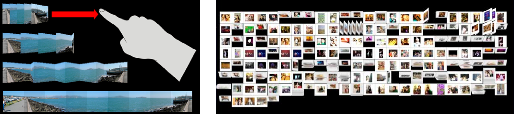
\includegraphics[width=\textwidth]{imgs-RelatedWork/hsu.png}
	\caption[Hsu's work of grouping together related images]{On the left, an example of an interaction on a group of photos that makes a panorama. On the right, a visualization on 537 photos with some groups.}
	\label{fig:hsu1}
\end{figure}


% section hsu:2009p2696 (end)

\subsection{A next generation browsing environment for large image repositories} % (fold)
\label{sub:Schaefer}

\begin{figure}[ht]
	\centering
		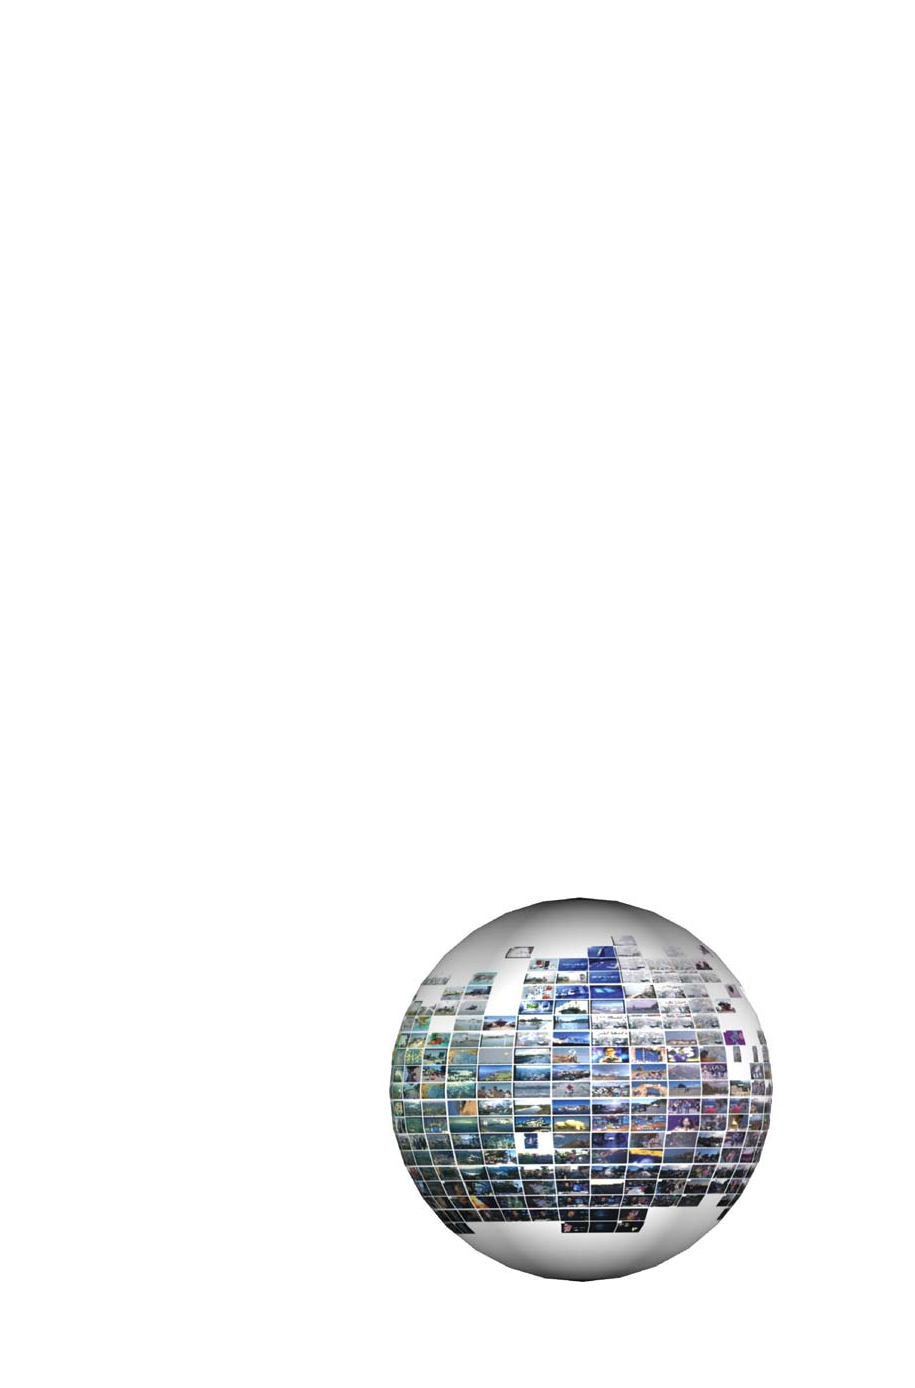
\includegraphics[scale=1]{imgs-RelatedWork/shaefer1.pdf}
	\caption{Hue sphere of a dataset, from Schaefer's work.}
	\label{fig:schaefer1}
\end{figure}

Schaefer \cite{Schaefer:2010p1871} tries to take similarity based organization of images from the 2D space to a 3D sphere, which allows interaction from the users. Rotating the sphere reveals images with different colors while tilting it reveals brighter or darker images.

Large image collections are handled through a hierarchical approach that brings up similar, previously hidden, images when zooming in on an area.

The description of the color is retrieved by calculating the image's median color for it's efficiency over other methods like histograms. This two features are directly mapped onto the sphere's coordinates and the entire structure is pre-calculated so browsing can be performed in real-time. Image overlapping is also avoided (\fig{schaefer1}).

The work was tested on a 4500 image collection with no evaluation as to its performance and a weak and subjective user testing.


% section schaefer:2010p1871 (end)

\subsection{Flexible access to photo libraries via time place, tags, and visual features} % (fold)
\label{sub:Girgensohn}
\begin{figure}[ht]
	\centering
		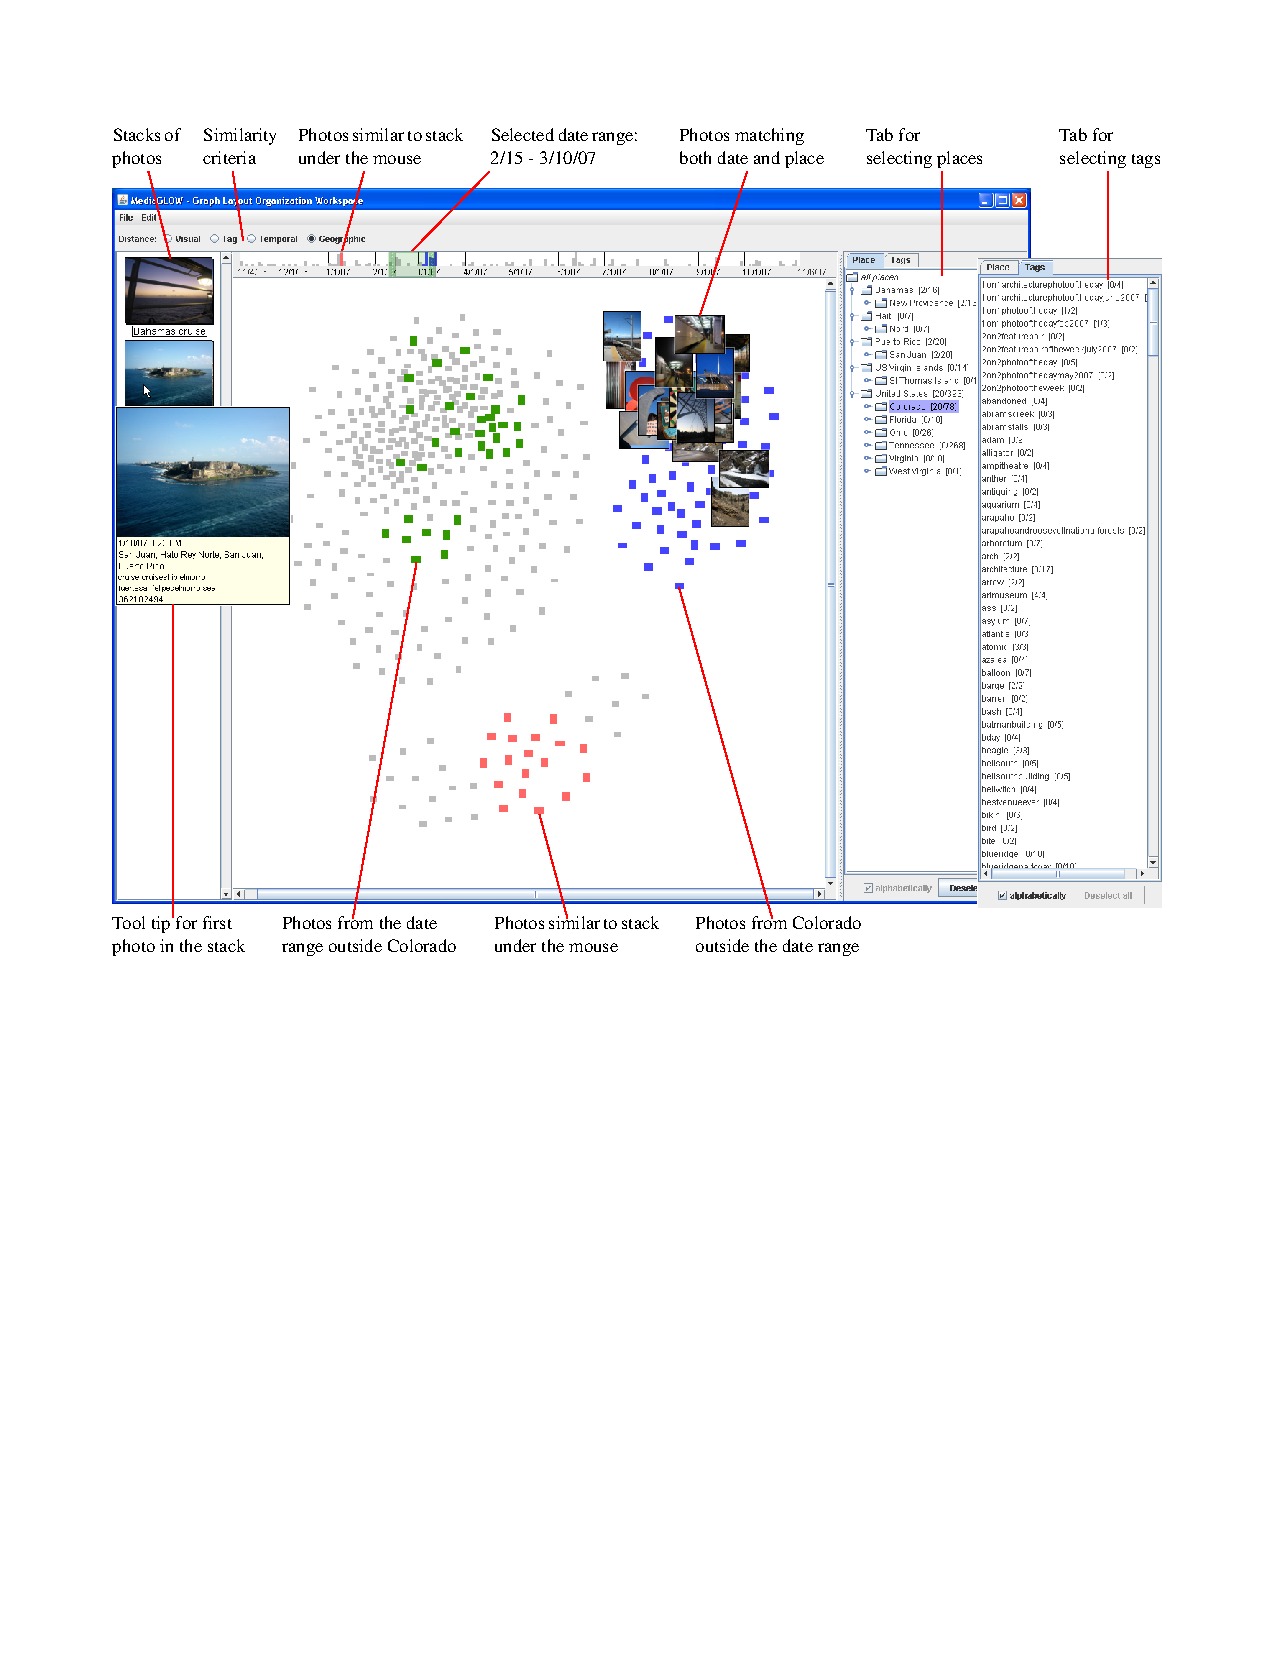
\includegraphics[width=\textwidth]{imgs-RelatedWork/Girgensohn1.pdf}
	\caption{Photos grouped by geographic similarity and filtered by date and place.}
	\label{fig:girgensohn}
\end{figure}

MediaGLOW by Girgensohn et al. \cite{Girgensohn:2010} is the application discussed in this paper. It's a \ac{CBIR} system with multiple ways to filter and sort the image collection.

The interface allows selecting a range of dates, places and tags at any time to filter the collection and the display will show the photos that match the filters, alongside indications of the existence of photos that match some of the filters. This display can then be arranged by four similarity criteria: temporal (by photo creation time), geographic (distances between places), tags (photos with similar tags are shown closer together) and visual (\fig{girgensohn}).

The time is selected using a timeline on the top of the screen while tags and places are shown on the right side sorted alphabetically, by frequency of, in case of places, as a tree. Multiple selections are allowed to show more photos.

The photo display is graph based, allowing for overlapped images. Various metaphors were developed to ease the navigation of the collection. Zooming is allowed and changes both thumbnail positions and size for better experience, allowing the photos to spread away from each other, but also increasing the size so the user can have a better look at them. The authors think that bigger thumbnails and a correct grouping of related photos is more important than spreading them to avoid the overlapping problem.

Color coding is used throughout the interface to help the user understand better what is being selected. For instance, on the timeline blue and grey are used to distinguish photos that match or not the selected location/tag. On the photo display, besides the photos that are actually shown are colored blocks: blue for photos that match location only, green for time only and grey for those that didn't match anything.

Detailed user testing was performed and the importance of the multiple ways to organize and search the collections was emphasized since many systems are designed to have a single form of access. Some users also pointed the importance of being able to have a non overlapping view of the photos for part of the task.

Each view was found to have different levels of usage, the geographic being the most used and temporal the least, since it's very similar to the timeline. Visual similarity was less used than expected, even on collections where it was relevant. 




\subsection{PhotoMesa: a zoomable image browser using quantum treemaps and bubblemaps}
\label{sub:PhotoMesa}

This work presents PhotoMesa by B. B. Bederson \cite{Bederson:2001:PZI:502348.502359}, an application that supports browsing sets of images in a zoomable environment. It also supports clustering by metadata, not requiring previous work from the user. Users can choose directories of images and they are all displayed in a space-filling manner \fig{photomesa}. Images are displayed in groups, from the directories they origin from and users can smoothly zoom in to a group and then to a single image. It generates multiple-resolution thumbnails for maintaing a good performance. Keyboard keys are also used to navigate the canvas. The groups display their name and have different background colors for a better distinction. It also supports drag and drop of images to other applications. Text search is possible as well as selecting a group on a list.

\begin{figure}[ht!]
	\centering
		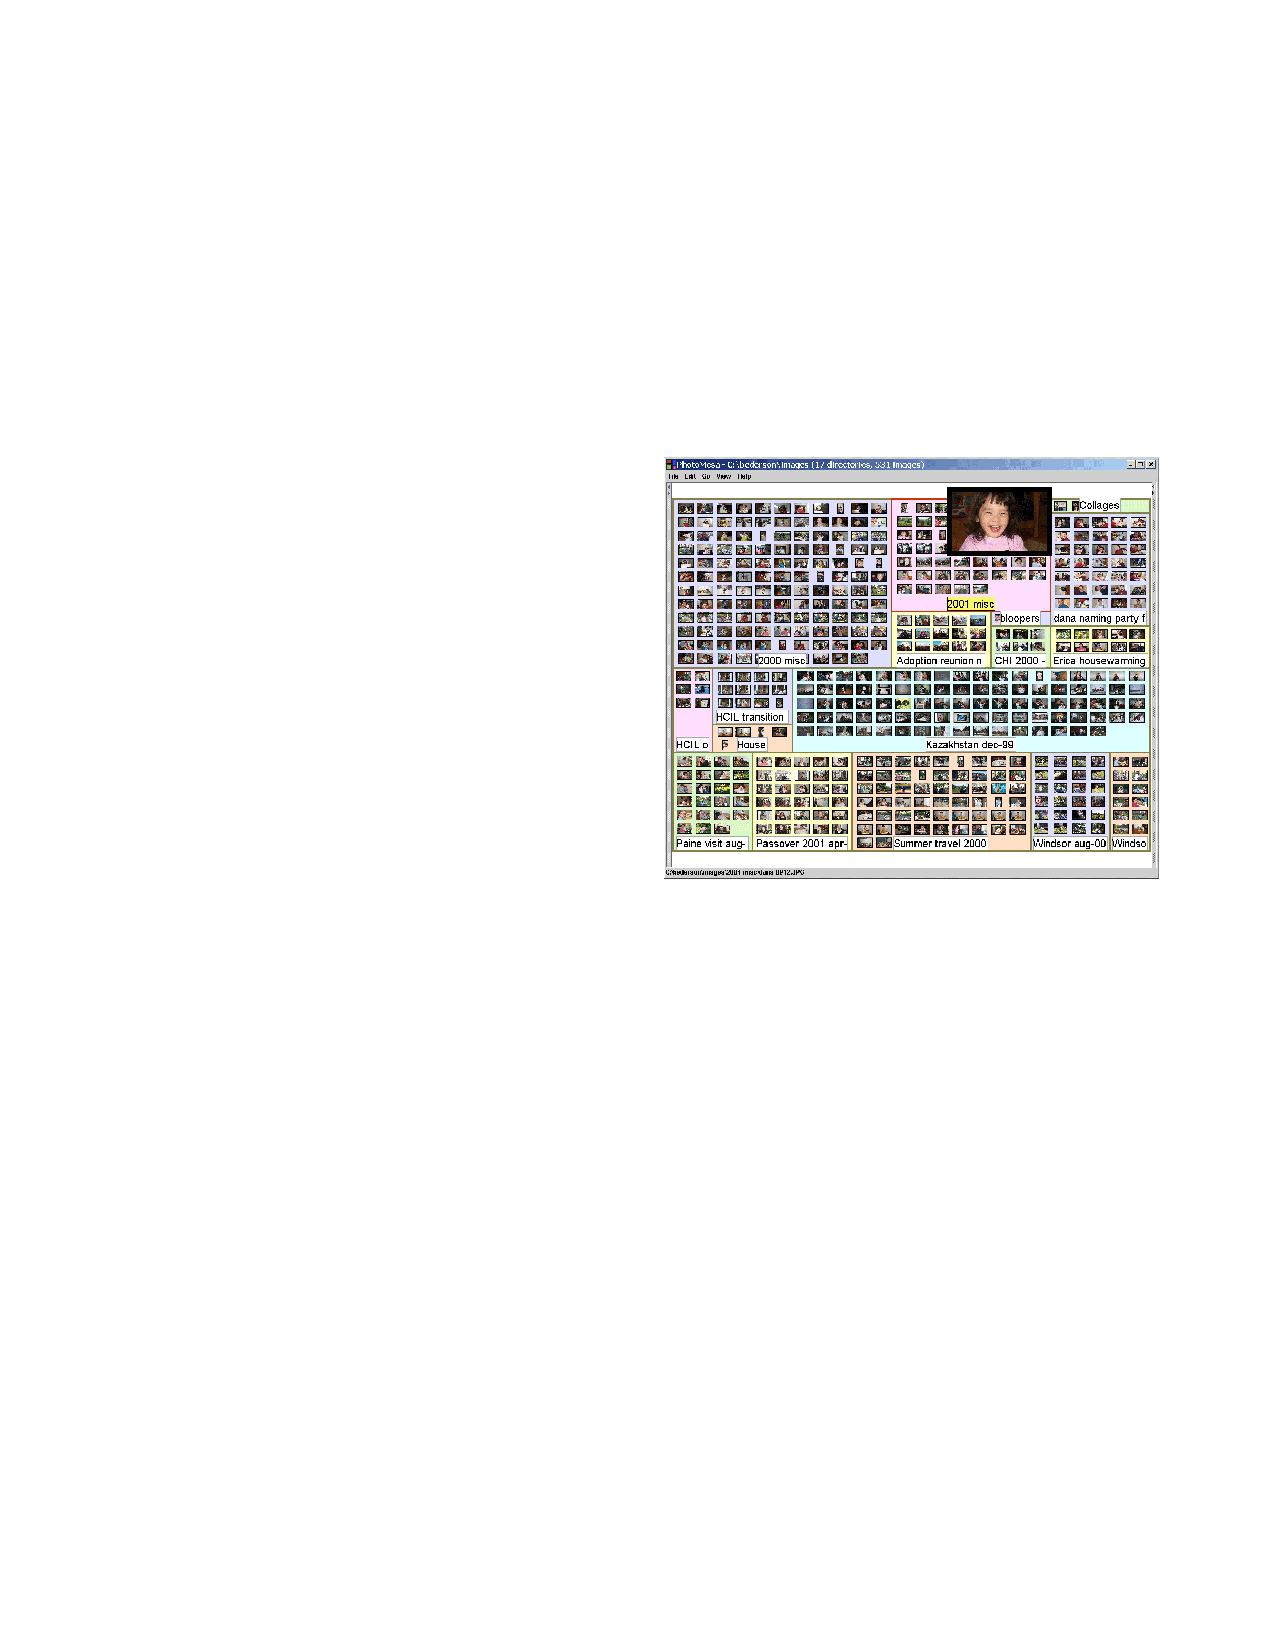
\includegraphics[width=0.90\textwidth]{imgs-RelatedWork/PhotoMesa.pdf}
	\caption{PhotoMesa with over 500 images in 17 groups.}
	\label{fig:photomesa}
\end{figure}

PhotoMesa implements two algorithms for space filling, one is Quantum Treemaps by the author, a variation of the Ordered Treemap  that is aware of the constraints imposed by the use of images, like grid alignment and common size, and Bubble Maps which is designed to have the least wasted space possible.

This work brings very interesting ideas to the table, but it has a somewhat limited reach, with only referring to ``over 500 images'' on the application and by only taking simple metadata, like the path and modification date of images.




% section girgensohn:2010 (end)

\section{Discussion} % (fold)
\label{sub:discussion}


Currently there are a lot of approaches to image organization and each has its own differences as demonstrated on Table \ref{tab:brows-meth}. Our survey went by multiple works and revealed various methods for extracting the features from each image, multiple visualization methods from grids to flying images.


\begin{table}[ht]
 \begin{tabular}{| m{2.7cm} |>{\centering}m{2.3cm}|c|c|c|>{\centering}m{2.1cm}|>{\centering}m{2.3cm}|r|}
  \hline
\multirow{2}{*}{\textbf{Work}} & \multicolumn{4}{c|}{\textbf{Organization}} & \multirow{2}{*}{\textbf{Visualization}} & \multirow{2}{*}{\textbf{Focus}} & \multirow{2}{*}{\textbf{Size}} \\
\cline{2-5}
	& \textbf{features} & \textbf{date} & \textbf{gps} & \textbf{tags} & & & \\

\hline 1.	Qiu \cite{Qiu:2007p1207}	& simple color measures 			& --- & --- & --- & Grid 			   & Simplicity and Efficiency 			& 60,000	\\
\hline 2.	Rodden \cite{Rodden:2001p731}	& --- 								& --- & --- & \cm & Grid 			   & Similarity usefulness	 			& 	 100	\\
\hline 3.	Porta \cite{Porta:2006p416}	& --- 								& --- & --- & --- & Spot (and others)  & Unconventional visualizations		& 	 400	\\
\hline 4.	Cooper \cite{Cooper:2006p543}	& --- 								& --- & --- & --- & Static and animated& Usefulness of animations 			& 	 ---	\\
\hline 5.	Strong \cite{Strong:2009p413}	& color histograms and gradients 	& --- & --- & --- & \ac{SOM} 		   & Evaluation of different features	&  2,200 	\\
\hline 6.	Tan	\cite{Tan:2001p850}		& color histograms of subdivisions & --- & --- & --- & --- 			   & Evaluation of different features 	& 12,000 	\\
\hline 7.	Naaman	\cite{Naaman:2004p1802}	& --- 								& \cm & \cm & --- & --- 			   & Organization based on events 		& 	   N/A	\\
\hline 8.	Chen	\cite{Chen:1998p2344}	& colors, edges and textures 		& --- & --- & --- & --- 			   & Efficient fast-sparce clustering 	& 10,000 	\\
\hline 9.	Heesch	\cite{Heesch:2004p2675} & six different features 			& --- & --- & \cm & Radial 			   & Complex similarity network 		& 32,000 	\\
\hline 10.	Phorigami, Hsu	\cite{Hsu:2009p2696}	& --- 								& --- & --- & --- & Grid with groups   & Interaction on grupped photos 		&  1,333 	\\
\hline 11.	Schaefer \cite{Schaefer:2010p1871} & color histograms of subdivisions & --- & --- & --- & 3D Sphere		   & 3D mapping and interaction 		&  4,500 	\\
\hline 12.	MediaGLOW, Girgensohn \cite{Girgensohn:2010}	& --- 								& \cm & \cm & \cm & Overlapped graph   & Having the best way to find photos &    450	\\
\hline 13. PhotoMesa, Bederson \cite{Bederson:2001:PZI:502348.502359} & --- & \cm & --- & \cm & Q. Treemap / Bubblemap & Zoomable browser & 500	\\
\hline
 \end{tabular}
\caption{Different browsing methods}
\label{tab:brows-meth}
\end{table}

One of the main problems is obtaining useful information from low level feature extraction of the image contents. Some try to get the most out of each image, with a variety of complex and time consuming procedures, e.g., a variety of methods based on color histograms \cite{Strong:2009p413,Tan:2001p850,Chen:1998p2344,Schaefer:2010p1871} or even more detailed ones with textures and convolution filters \cite{Heesch:2004p2675}. Others try to focus on avoiding the complex computations by only getting simple, but somewhat useful information \cite{Qiu:2007p1207}. To contrast with these methods, Girgensohn's work \cite{Girgensohn:2010} has found that users prefer other ways to filter the collection, like tags, dates and locations. Low level features are still used, but they have to be kept to understandable and useful options.

Date and location are simple similarity measures and can be used to group the collections by events and locations like Naaman did on this work \cite{Naaman:2004p1802}. Current mainstream software like Apple's iPhoto\footnote{http://www.apple.com/iphoto} or Google's Picasa\footnote{http://picasa.google.com} are already doing it in a semi-automatic way.

Textual metadata like tags and descriptions are also widely used both on our survey \cite{Rodden:2001p731,Girgensohn:2010,Heesch:2004p2675,Bederson:2001:PZI:502348.502359} and on all mainstream software. The problem with tags and descriptions is that people usually don't assign them to their photos, but that's not a problem we're interested here.

The visualization is the field with most variations and experimentations, like Porta's work \cite{Porta:2006p416} where multiple options were tested, but only a couple of the most simple were considered useful. The 3D Sphere \cite{Schaefer:2010p1871} is also visually interesting, but doesn't provide a better interface to the collection since it's based on a grid view, but hiding many images on the far side of the sphere. The Phorigami work \cite{Hsu:2009p2696} introduces some interesting metaphors for reducing the space occupied by some groups of photos, but some make the visualization harder and could, therefore, be improved.

Girgensohn and Bederson's works are among the most interesting and relevant to our vision. MediaGLOW's \cite{Girgensohn:2010} visualization approach allows images to be organized by various features and to be filtered down, displaying matched photos alongside placeholders for photos that are only match partially. The timeline on the top is also very useful. It has some problems like image overlap and capacity for showing large collections, but the ideas are still interesting. PhotoMesa \cite{Bederson:2001:PZI:502348.502359} has a visualization style close to what we want from our work, but its reach is short, i.e., has a small set of features and dispositions, doesn't handle many images and the \ac{UI} seems a little cluttered with all the strong colors and borders.

The seemingly more useful exploration tools are the ones that handle less images, which seems like a contradiction. The more images a system can hold and efficiently display, the more useful it gets. From our user survey (appendix \ref{appendix:usersurvey}), we learnt two thirds of people have less than 10 000 photos (\ref{ssub:library_size}) and we will do our best to reach that level.

% section discussion (end)
% chapter related-work (end)
\chapter{Solution Requirements} % (fold)
\label{chapter:solution_requirements}

Our survey was based on various types of previous work from the last ten years. Image browsers and technology have evolved a lot since then, but there still isn't a definitive way for a user to look at his larger photo collection and understand its content and evolution.



We have the vision of a system that displays a large set of user’s photos at the same time, in various arrangements, revealing patterns, differences and similarities between them.

We will now expose this vision by presenting the main goals we want to achieve with this thesis, as well as some of the guiding implementation requirements that we followed for a better end result.





\section{Main Goals} % (fold)
\label{reqs:main_goal}

The main goal of this thesis is to provide a different approach to the photo collection browsing methods. More specifically, the work should:


\subsubsection{Extract interesting information about the images}
We want to be able to organize and classify images. As we have seen on the Related Work, there are many ways to extract information from images, some simple, some complex. We have chosen a few that we think are the most relevant to the scope of our work. We will explain what we chose and why below, in section \ref{reqs:features}.


\subsubsection{Provide an interaction with the full set of images}
We want to enable the users to easily view and interact with the all the images at the same time, if they want to, instead of just limiting to a small window of images. Many of the Related Work did this and displayed all images at the same time \cite{Qiu:2007p1207,Chen:1998p2344,Girgensohn:2009:MOP:1502650.1502711,Bederson:2001:PZI:502348.502359}. Others only displayed a subset of images, but we think the users should have the power to create and view their own subsets from the full one.


\subsubsection{Efficiently display a large number of images in a single screen} % (fold)
This goal goes inline with the previous one: to be able to interact with a large set of images, we should be able to display them all, at the same time, using techniques to make better use of available screen space. We saw different ways to display images on the Related Work, some focused on displaying images efficiently \cite{Qiu:2007p1207,Rodden:2001p731,Naaman:2004p1802,Hsu:2009p2696,Bederson:2001:PZI:502348.502359}, others more focused on the relations between the images \cite{Girgensohn:2009:MOP:1502650.1502711,Heesch:2004p2675}. Hsu's work \cite{Hsu:2009p2696} is specially interesting for its idea of merging images that were related and we want to include this in our work, but with an automatic way of grouping and a clearer \ac{UI}.

\subsubsection{Allow the manipulation of the display}
We want the users to create different views that enable new perceptions of their collection, based on the extracted information. Many works allowed some sort of highlight \cite{Girgensohn:2009:MOP:1502650.1502711}, zoom \cite{Bederson:2001:PZI:502348.502359} or similarity filter \cite{Qiu:2007p1207,Heesch:2004p2675}. Some are more useful then others and we think we should apply them sensibly. Since we are going to display a large amount of images at a small size, there will be the need to increase the size of the images, therefore we require the ability to zoom in on images and to provide some filters for any available data, but also for custom user selections. It is also interesting to have some similarity filtering.
	
\vspace{\baselineskip}
	
With this capabilities, our work should be able to provide the user not only a better understanding of the collection, but also with an easy and interesting way to visually combine and view photographs.


%be able to handle thousands of images and display them all on the screen while maintaining responsiveness and giving useful information. The system's \ac{UI} should be clear and easy to use, allowing the user to navigate through the display of photos, through zooming and panning, and to reorganize the display the photos in a number of ways.

%The system should also gather as much information as it can from the photos, such as date and time, relevant colors, presence of people, type of photograph, user organization or location. While some of this information is already embedded in today's digital photographs as metadata, written by the digital camera when the photo was taken, others are usually not and need to be calculated or extracted. Faces and relevant color information are an example of that and the system must be prepared to extract this features from the image. The system must provide some capability for other feature extraction methods to be easily added in the future. All this information will then be used by the user to reorganize and filter the photos on display.


%§ We will now detail the work done, taking this requirements into account.

% subsection main_goal (end)









\section{Implementation Requirements} % (fold)
\label{reqs:Implementation_Requirements}

In addition to the referred main goals, we set ourselves some design goals, or requirements, for our implementation. With them, we want our work to get closer to a real application, that real users can use and have some flexibility for it to evolve with time.

Therefore, we set the following requirements:

\subsubsection{Ease of Use} % (fold)
\label{reqs:ease_of_use}

Ease of use is one of the most important characteristics of any piece of software and can shape how well it will sell. Much more attention has been given to the \ac{UX} in the last few years. Systems that are easier to use, get the job done faster, are more enjoyable to use and allow less experienced users to use them.

Since this is such an important characteristic, we aimed at providing a simple interaction from the beginning to the end, while also providing a powerful system, even though it could be even more refined in a few areas.

% subsubsection ease_of_use (end)



\subsubsection{Extensibility} % (fold)
\label{reqs:Extensibility}

The extensibility factor of a system is also important for the added value that can be obtained by quickly adding new features, either by the developers or by third parties. We made some parts of our work with this in mind, by allowing either external plugins or by generalization of code, allowing for future improvements with less trouble.

% subsubsection Extensibility (end)



\subsubsection{Performance} % (fold)
\label{reqs:Performance}

One of our main goals is to display a large set of images on the screen, but this brings problems since each image, in full-size, can take a good set of resources of the system. If we multiply this resources for a thousand images, we will not have a performent work.

Therefore, we set this requirement for having a performent work, that can be used with at least a few thousand images without taking down the system while using it.
% subsubsection Performance (end)




\subsubsection{Persistency}

Our system will spend sometime generating and gathering data for each of the available feature extractors, for each image. To avoid having to re-do work in case of a failure, addition of more images to the collection or stopping to resume later, the system must store the data after its generation. This should be accomplished using a system wide framework to provide easy storing of all the data. Since this work is intended to be an exploration of visualization concepts, so we will not support interoperability from our system to others by using MPEG-7 or other metadata descriptor standards, but instead use something that is simpler to implement.


% subsection design_goal (end)




\section{Features of Images and Photographs}
\label{reqs:features}

%extract interesting information about the images
As referred before, we want our system to extract interesting information about the images and we will now explain this in detail.


Unlike textual data, images are a type of data where is not trivial to extract information from, in a computational environment. It's easy for us, common people, to understand what certain picture is showing. We can easily distinguish if there are, for instance, animals, people, flowers or buildings, but it's hard for a computer to do the same, and it's even harder to understand if that certain photo of a building and a person was taken because of the building, the person or both.

There have been various developments in the feature extraction front \cite{Liu:2007p3740,Datta:2005p3749,Rui:1999p949} and is currently possible to perform various detections in images with various levels of satisfaction.

Some examples of working solutions for feature detection:

\subsubsection{Face recognition}
Detection of the presence of faces in the images, their position and relations between them as some other works refer \cite{Vasconcelos:2005in,Chen:2003p3699,Tamura:2002p859,Hsu:2002p3675}. Face recognition has been gaining public appreciation in the past few years since many photo applications and services have been including it. Our user survey reflects that people like this feature and request it (\ref{ssub:suggestions_of_features}). The problem with face recognition is that it requires users to identify who are the persons on each photo which, generally, is a long and repetitive process. For concept, we will only detect the presence of faces and not spend time identifying them.

\subsubsection{Object recognition}
Identification objects in images. This is a useful extractor, but is requires a huge library of sample imagery for comparison \cite{Torralba:2008p527} and it's not feasible to adopt in our work.
	
	
\subsubsection{Identification of perceptive colors}
What are the main colors that users perceive in certain image \cite{Sural:2002bt,Tan:2001p850}. An image is composed of different colors or tones and people can identify images by their main colors and dispositions. There are simple ways, like calculating the mean color for an image, but that's not faithful. Detecting perceptive colors identifies the different colors of an image, providing more realistic data.

\subsubsection{Image sequences}
Identification of images of the same scene that were taken in sequence, for grouping purposes \cite{Cooper:2003p3679}. Images taken in sequence of the same subject should be gathered into a group of images, with the purpose of reducing the needed space to display them. This is important since almost half of the people we inquired on our survey claims to use techniques that capture a great number of photos sequentially (\ref{ssub:photos_in_close_sequence}). This can be either by looking at the capture date or by analyzing the visual similarities of sequential images.

\subsubsection{Image similarity}
Identification of similar images across the whole collection enabling a search of similar images from a selected one or just grouping similar images according to defined parameters. There are many ways of doing similarity, some simple, like measuring the average color of the image \cite{Strong:2009p413,Qiu:2007p1207,Schaefer:2010p1871}, some complex like measuring various color attributes, edges, textures, applying filters or using convulsion like Heesch \cite{Heesch:2004p2675} and Chen \cite{Chen:1998p2344} did. For our work, we will explore options for color similarity, paving the way for other more accurate methods.

\vspace{0.5\baselineskip}

We want to use some of this methods to automatically extract information from the contents of images but, since this work is mostly focused on photography, there is another way to obtain really useful information that is EXIF Metadata. None of the related works seemed to use it, although users are interested in them, as can be seen on our user survey (\ref{ssub:preferred_features}\hide{ and \ref{ssub:suggestions_of_features}}).

EXIF Metadata is a standard format for metadata included in digitally captured media, like photographs captured by digital cameras. This devices save a lot of information on the image file, like the date and time of the capture, camera settings, camera orientation, location data and even detected faces\footnote{the availability of some of this data requires capable camera hardware and software that are getting more common nowadays.}. An example of the metadata fields can be seen on Table \ref{tab:exif}. This is textual data and, therefore, much faster and easier to retrieve and analyze than the content based methods we discussed above, being a great addition to them.

Mixing all this different data, users should be able to interact, filter, sort and organize their collection in various ways, obtaining new and different perspectives of their images.

\begin{table}[h]
\vspace{\baselineskip}
\renewcommand{\arraystretch}{1.4}
\rowcolors{2}{light-gray}{white}
\centering
\vspace{0.2cm}
	\begin{tabular}{ll}
	\textbf{Field Name}			&	\textbf{Example Value}\\
	\hline
	Camera:				&	Canon PowerShot S5 IS\\
	Exposure:			&	0.017 sec (1/60)\\
	Aperture:			&	f/3.2\\
	Focal Length:		&	6 mm\\
	ISO Speed:			&	80\\
	Exposure Bias:		&	-2/3 EV\\
	Flash:				&	Off, Did not fire\\
	Software:			&	Adobe Photoshop Lightroom 3.4\\
	Max Aperture Value:	&	2.7\\
	Subject Distance:	&	0.3 m\\
	Metering Mode:		&	Multi-segment\\
	Sensing Method:		&	One-chip color area\\
	Custom Rendered:	&	Normal\\
	Exposure Mode:		&	Manual\\
	White Balance:		&	Auto\\
	Keywords:			&	``Beach", ``Sand", ``Castles"\\
	Date and Time:		&	2010:09:18 11:52:59\\
	Lens:				&	6.0-72.0 mm\\
	Approximated Focus Distance:	&	0.3\\
	Flash Mode:			&	Off\\
	Metadata Date:		&	2011:06:14 20:03:04+01:00\\
	GPS Latitude: 		&	38 deg 52' 47.67" N\\
	GPS Longitude: 		&	9 deg 9' 47.13" W\\
	GPS Altitude Ref: 	&	Above Sea Level\\
	GPS Altitude: 		&	214.9 m\\
	GPS Date Time:		&	2010:09:18 10:52:59\\
\end{tabular}
\caption{Example of some relevant EXIF fields imprinted by the camera and by the computer software used for post processing.}
\label{tab:exif}
\end{table}



% chapter solution_requirements (end)
\chapter{Eagle Eye}
\label{cha:eagle_eye}

% 30/40 pages

Eagle Eye is a visualization tool that enables the display and manipulation of a large image set at once. It is focused at the regular computer user that has a few thousand digital photographs stored on the computer. It allows navigation, through panning and zooming the canvas of the image collection, sorting through different methods and multiple ways of filtering, either textual or visual.

We will now explain what makes all of this work.


\section{Design Decisions} % (fold)
\label{sub:design_decisions}

\subsubsection{DeepZoom} % (fold)
\label{ssub:deepzoom}

After analyzing some visualization technologies that allowed easy display and manipulation of images\todo{Insert a bunch of useless tech}, Microsoft’s Silverlight, with its DeepZoom technology, proved to be the best choice.

DeepZoom enables the use of multiple resolution images for efficient display at various zoom levels and, for instance, is used for the display of gigapixel photos\todo{links}, where the user can view the whole image or zoom in the small details, or for collections of photos where the user can zoom between a view of multiple images and the details of a single image. So far, usages of DeepZoom have been restricted to promotion websites, art galleries and other closed usages.

\red{This should be about the multi-scale images and not about DeepZoom $\rightarrow$ }Our work aims at bringing this technology to the regular user, in a much simpler and dynamic way.

Although DeepZoom seemed a great technology, it relies on Silverlight, which by itself isn't as good as using a full-fledged desktop application framework like \ac{WPF} or other frameworks native to their platforms. This created some undesired limitations like the need to have two separated parts of the system, the visualization and the backend, and other smaller problems like limited access to the disk from the visualization part.

To create a DeepZoom application, some pre-processing is required before hand to create multiple versions of each image in various resolutions and also to create imagery of a global view of the collection, also in multiple resolutions. This enables DeepZoom to only load the appropriate set of images for a certain zoom state, keeping the bandwidth (if used on the Internet) and memory \red{requirements} to a manageable level. This required pre-processing   is done once on the backend. The visualization then uses the generated data to display the collection, being, at this point, totally independent from the original image files belonging to the user.

% subsubsection deepzoom (end)
% subsection design_decisions (end)

\section{Backend} % (fold)
\label{sub:backend}

The backend is one of the two parts that make Eagle Eye. Its purpose is to extract information from images and set everything up for the Visualization.

Currently it is a command line utility that allows the user to enter paths for folders containing image files. The system will then read those images, gather their metadata, process them with the existing plugins to extract visual features and, finally, generate and output the multi-scale imagery \red{(ainda não se falou disto)} alongside with control metadata for the visualization.

We will now detail its architecture, and implemented feature extractors.

\subsection{Architecture of the Backend}

The Backend comprises a library manager to hold the images, feature extractors to process those images and persistence to save all generated data.

Figure \ref{fig:arch} is a simple explanation of the components. The Eagle Eye part is the main application, containing the library and feature extractor managers. Both deal with files on the disk, JPEG image files and DLL extractor plugins, respectively. The user interacts with the core of Eagle Eye which currently provides a command line interface for its actions, like the image import and plugin execution. The import gathers the files and their metadata, to be later accessed by the plugins for processing. Plugins store the resulting data inside the library manager and can be accessed afterwards for outputting by a special plugin.

We will now go through this components in more detail. 

\begin{figure}[ht]
	\centering
		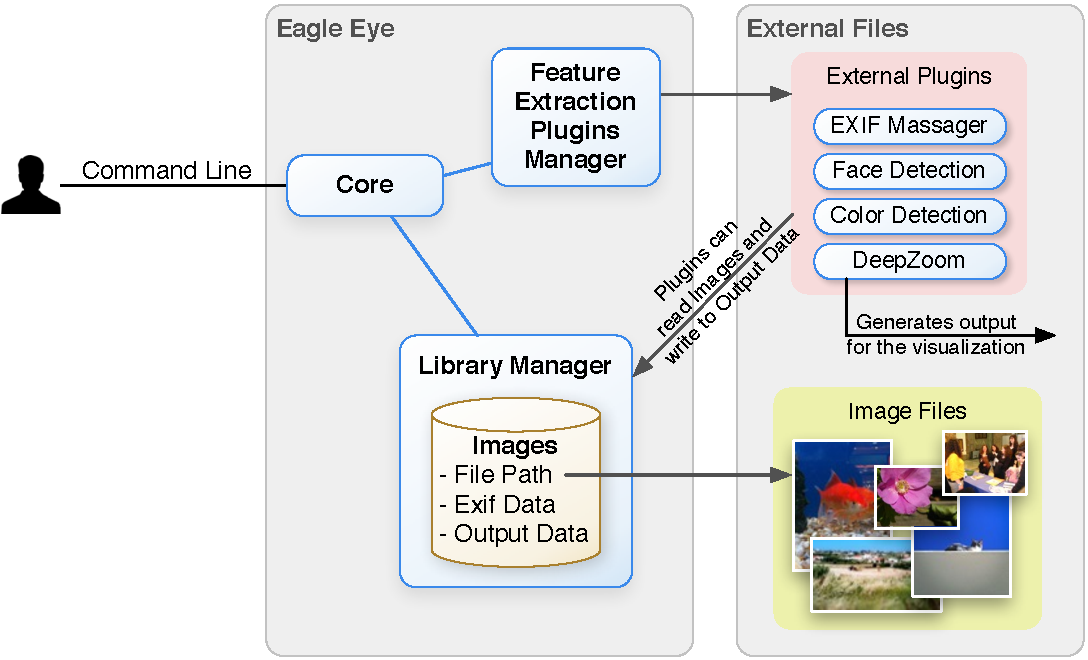
\includegraphics[scale=0.7]{Figures/Architecture_v2.pdf}
	\caption{Basic architecture of Eagle Eye's backend}
	\label{fig:arch}
\end{figure}


\subsubsection{Library Manager} % (fold)
\label{ssub:library_manager}

The system displays images and, therefore, it needs to know what to show. This is where the library manager comes in. It creates a database which indexes existing JPEG image files stored on the user's computer and makes this information available for other modules to use. It is designed to be used with digital photographs which contain the aforementioned EXIF metadata like time, date, camera information, or location. This information is gathered upon import and is available throughout the Backend.

We explored a few ways to develop the image import process and we rested at the fastest we found. The user refers a folder to be imported and we use a third-party program, ExifTool\footnote{ExifTool is a utility that allows easy read and write of file metadata. \url{http://www.sno.phy.queensu.ca/~phil/exiftool}}, to crawl through the user-specified folders while identifying all the JPEG images and returning their \ac{EXIF} metadata which is then stored by our system (\fig{arch:import}).

\begin{figure}[ht]
	\centering
		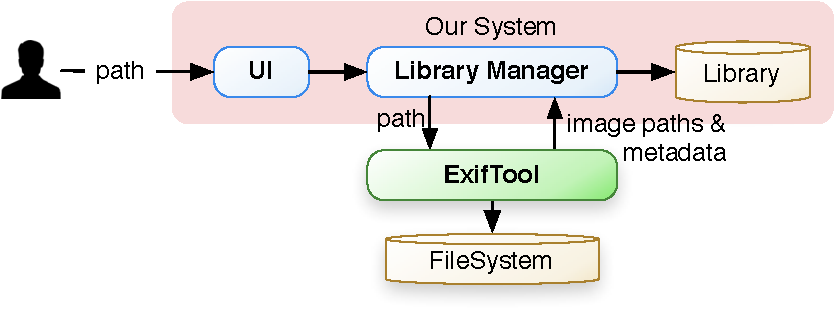
\includegraphics[scale=0.6]{Figures/import.pdf}
	\caption{Process in use by our system of importing a folder using ExifTool.}
	\label{fig:arch:import}
\end{figure}


Another option for importing metadata was to invoke ExifTool as part of a \ac{FEP}. Although that could fix a couple of problems with the current  implementation, it doesn’t make the metadata as ubiquitous as needed. Most \acp{FEP} rely on some \ac{EXIF} plugins to work correctly and the current implementation doesn’t easily allow inter-\ac{FEP} data-sharing.

% subsubsection library_manager (end)




\subsubsection{Feature Extraction} % (fold)
\label{ssub:FeatureExtraction}

To enable the Visualization to arrange the images on the screen in different ways, they need to be classified. Some information is easy to obtain and compare, like when the photograph was taken. Other information needs to be extracted, like the number of people in the photo or what are the most relevant colors in the image. \Fig{fe} is a short example of what feature extraction is all about.

\begin{figure}[ht]
	\centering
		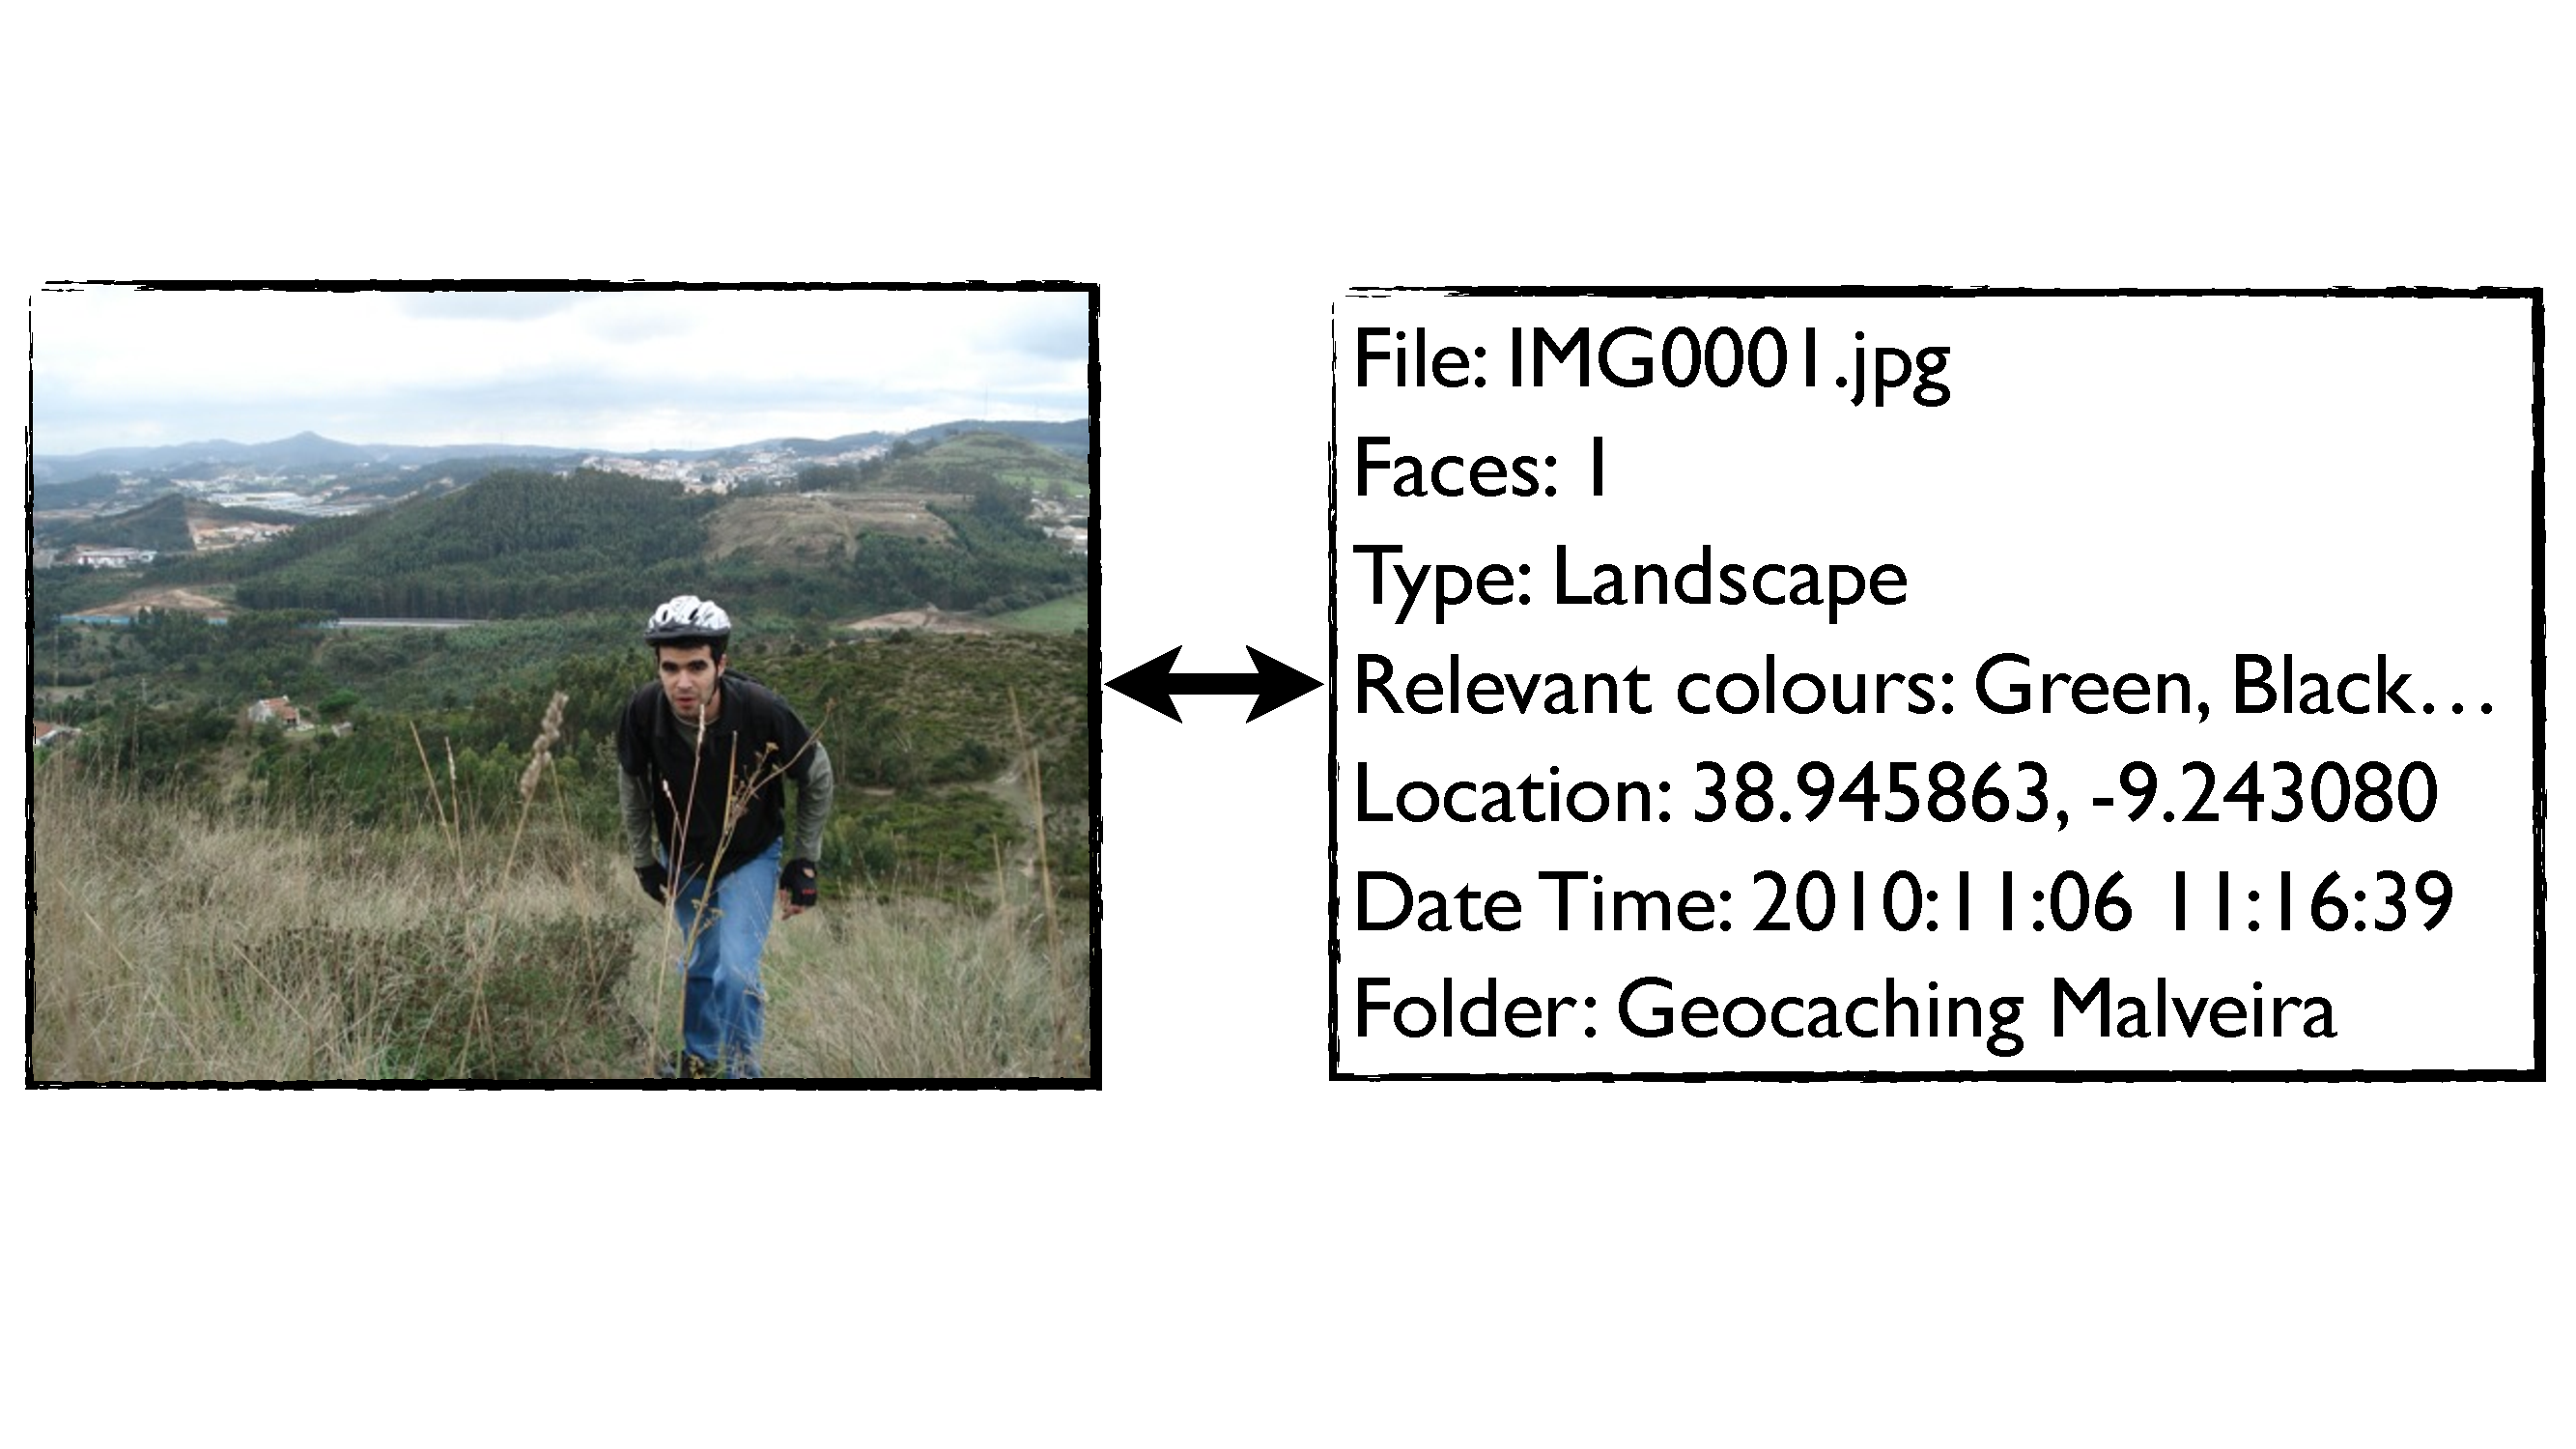
\includegraphics[width=0.72\columnwidth]{Figures/fe.pdf}
	\caption{Example of information extracted from an image.}
	\label{fig:fe}
\end{figure}

We had a few ideas for extracting features from images and, to be possible to add more along the way, we developed a plugin system to ease the creation of other feature extractors in the future.

Each Feature Extraction Plugin is separated from the main system. They need to implement a common interface and are given the ability to access the image data from the library, and save the computed data back. They have freedom to access the image file or its \ac{EXIF} information. They should, in the end, store the processed data in a specified way so it gets exported to the visualization. Implemented plugins will be explained in section \ref{sub:plugins}.

% subsubsection Feature Extraction (end)




\subsubsection{Persistence} % (fold)
\label{ssub:Persistence}

Persistence of both library and plugin data are required so the system doesn't lose information that took time to generate. To ease the interaction with a database system, we created a database abstraction layer that hides the complexities of interacting with said system. It also allows us to change to another database system if we see the need for it. We chose Oracle's Berkeley DB\footnote{Berkeley DB is a high-performace, embeddable, key-value, file-based database available at \url{http://www.oracle.com/technetwork/database/berkeleydb}} for its speed in retrieving data.

With this layer we can hide some optimization complexities like lazy-saving and lazy-loading. We use lazy-saving to save data to disk by chunks instead of doing it on each small update, speeding up the update process. Lazy-loading is not yet implemented but it is essential with libraries with tens of thousands of images, where keeping a complete library in memory is not feasible.

% subsubsection database_abstraction_layer (end)

%subsection arch backend (end)












\subsection{Feature Extraction Plugins} % (fold)
\label{sub:plugins}

Back in the Solution Requirements chapter (\ref{reqs:features}), we detailed some possible features that were interesting to be used in this work. In this section we will detail what extractors have been implemented.

Currently, we have four feature extraction plugins:
\begin{myitemize}
	\item Selection of useful image metadata
	\item Detection of image’s main color
	\item Face detection
	\item Generation of multi-scale imagery
\end{myitemize}

We now proceed to the explanation of each one of this plugins. 

\subsubsection{Selection of useful image metadata}

This plugin acts as a filter for all the available \ac{EXIF} tags. It picks the most relevant ones, codes them in a pre-defined way and appends them to the rest of the information to be exported for the visualization.

Information when the photo was captured, what device was used, the path where it resides or information about the location where the photo was taken are a good example of the most commonly relevant tags \todo{Ask users what other tags are relevant for them}. In the future, this set of extracted tags could be optionally set by the user.


\subsubsection{Detection of image’s main color}

Sometimes people don’t recall where or when a photo was taken, or where is it, but they vaguely remember that the photo had some dominant colors, like the red of a parrot in a green background (\fig{parrot}). This kind of information can be helpful when searching for a photo in a collection.

\begin{wrapfigure}{r}{0.3\textwidth}
	\vspace{-20pt}
	\begin{center}
		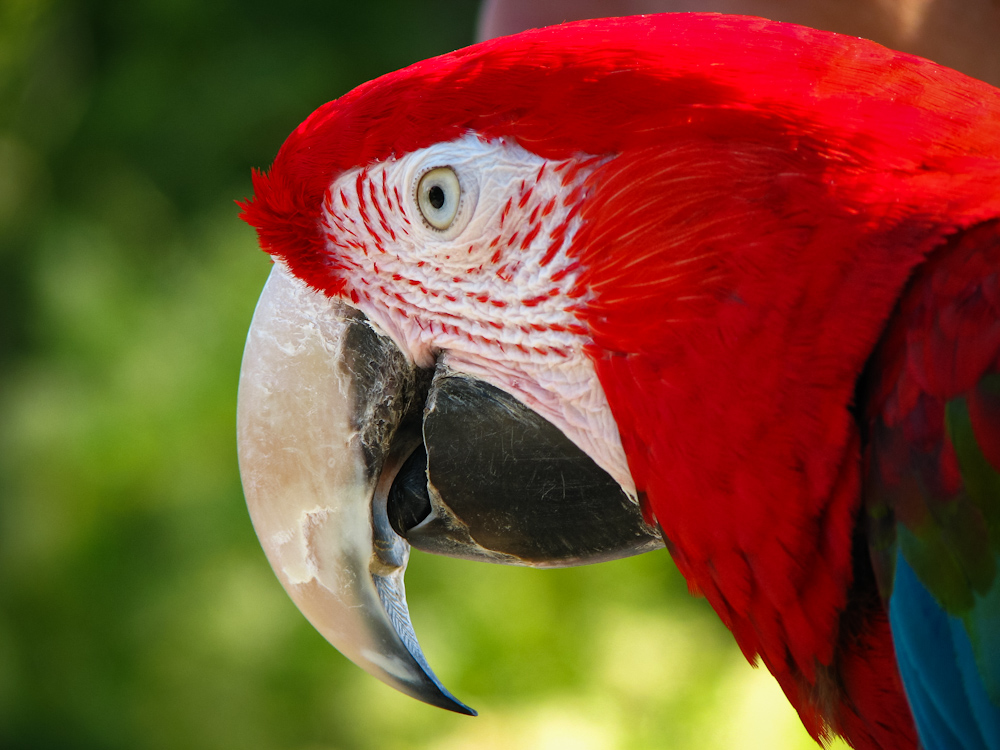
\includegraphics[width=0.29\textwidth]{Figures/parrot}
	\end{center}
	\vspace{-20pt}
	\caption{A colorful photo.}
	\vspace{-5pt}
	\label{fig:parrot}
\end{wrapfigure}

Color extraction from images has been a long standing problem \cite{Wan:2011bg,Strong:2009p413,Gabbouj:2009en,Girgensohn:2009:MOP:1502650.1502711,Zaheer:2010p3735,Datta:2008p1604,Chang:2007bt}. We wanted to extract the most perceptible colors from images so, in the parrot example (\fig{parrot}), the system should associate the image with the colors red, green, white and black and avoid colors that have little relevance, like the small blue of  the feathers and also ignore small tonal variances in the reds and greens.

For that we explored two methods that reduce the number of colors in an image to the most essential ones, the first being an adaptive method, selecting a few averaged colors from the image and the second using a palette as reference to select the colors.

A common JPEG photo can contain 16.8 million different colors. Our adaptive method reduces the possible colors to less than ten\footnote{We tried with multiple options from one color to ten colors and the results vary from image to image}. The obtained colors are chosen by averaging the colors in the image, so if there's a lot of blue tones, a single, averaged blue will be replacing those tones (see the middle image of \fig{sky}). In areas that have little tonal variation of the color, the resulting color will be very similar to the original (like in the right image of \fig{sky}). But sometimes this method fails to save important colors when they occupy a relatively small area of the image or if the image doesn't have a strong contrasts (shown by the left image in \fig{sky}).

\begin{figure}[ht]
	\centering
		\includegraphics[width=\columnwidth]{Figures/colorreduction.png}
	\caption{Three images where the left half is the original version and the right half is a version with very limited number of colors provided by the adaptive method.}
	\label{fig:sky}
\end{figure}




The second method uses a predefined color palette (\fig{colors}) which is an adapted mix between the eleven most recognizable colors (red, yellow, green, blue, purple, brown, orange, pink, black, white and grey)\footnote{Qiu \cite{Qiu:2007p1207} explains this are the most universal recognizable colors in any language.} and the 21 ColorAdd colors\footnote{ColorAdd is a 21 color catalog with symbols for each color designed specifically for color blind people. We used the colors as a reference, specially the light and dark variations.}. This mix has a great range of colors and each one can be easily named with recognizable words\footnote{We want to avoid names like ``Amaranth'' or ``Munsell'' that most people don't know about. A large list of this names can be found on \url{http://en.wikipedia.org/wiki/List_of_colors}.} which then could be assigned to the images. The images processed with this method get their colors changed to the most similar ones present in our palette. This assures that colors in a relatively small area or images with low contrast still get the deserved attention (\fig{pinkP}), unlike the adaptive method (\fig{pinkA}). This method doesn't reproduce the colors so well as the adaptive but, since we want to obtain generic colors, this one is more reliable.


\begin{figure}[!ht]
	\centering
		
\includegraphics[width=\columnwidth, height=45pt]{Figures/colours.pdf}
	\caption{Color palette in use for restricting the possible colors in an image.}
	\label{fig:colors}
\end{figure}


\begin{figure}[!htb]
  \begin{subfigmatrix}{3}
    \subfigure[Original image] {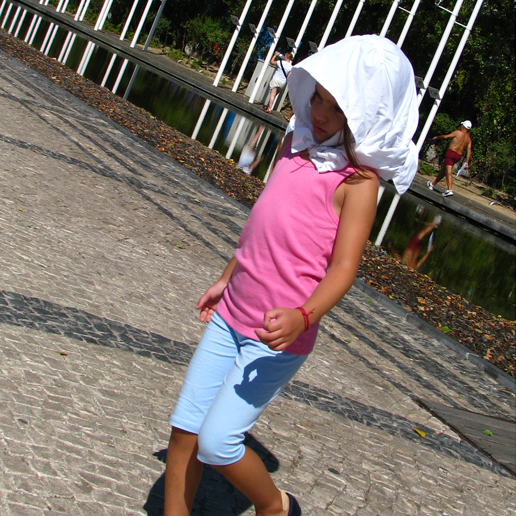
\includegraphics[width=0.328\linewidth]{Figures/pink1.png}\label{fig:pinkO}}
    \subfigure[Adaptive method]{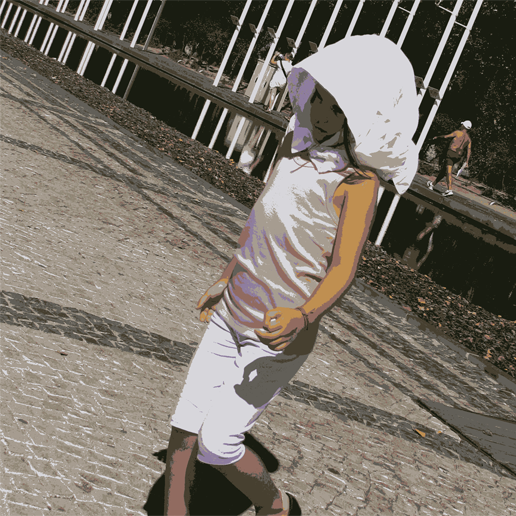
\includegraphics[width=0.328\linewidth]{Figures/pink2.png}\label{fig:pinkA}}
    \subfigure[Mapping method] {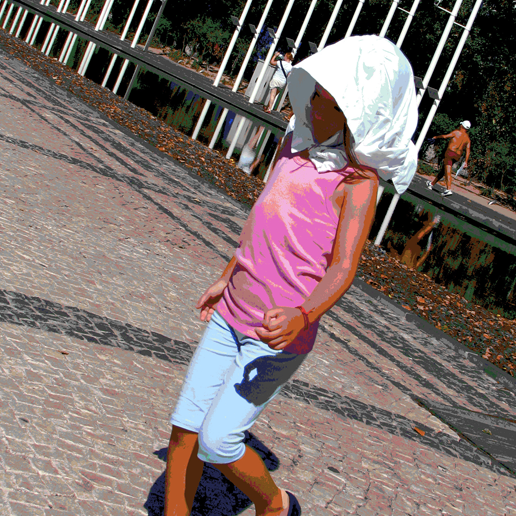
\includegraphics[width=0.328\linewidth]{Figures/pink3.png}\label{fig:pinkP}}
  \end{subfigmatrix}
  \caption{Comparison between the original image, the adaptive color reduction method failing to keep the pink and the blue colors and the color mapping method.}
  \label{fig:pink}
\end{figure}


This was the research we made to extract perceptible colors from images. We generated the above demonstration images using ImageMagick\footnote{ImageMagick is a software suite to create, edit, compose, or convert bitmap images. \url{http://www.imagemagick.org}} and its ``colors'' feature for the adaptive method and the ``remap'' for the palette method. Unfortunately, time was not on our side and we had to move to a simpler system. 

The current color extractor plugin does a simpler job of calculating the median color of the image and use the hue to index images.

We took some ideas from the work of Qiu et al\cite{Qiu:2007p1207} of exploring a method of image indexing that is fast and simple. On this work, images are sorted into ``bins'' according the their average color. This bins are divisions of color planes, indexed using binary trees allowing for very fast searches.

We used the open source library AForge.Imaging\footnote{AForge is a framework designed for developers and researchers in the fields of Computer Vision and Artificial Intelligence \url{http://www.aforgenet.com/framework/}} to obtain histograms for the images and compute their average color in RGB\footnote{Color model composed by red, green and blue \url{http://en.wikipedia.org/wiki/RGB}} and HSL\footnote{Color model composed of hue, saturation and luminance \url{http://en.wikipedia.org/wiki/HSL_and_HSV}} values. Both those values are then stored on the plugin-extracted data for each image. The images will be distributed into bins on the Visualization. We could assign bins at this point but, by not doing so, we are giving freedom to the users to change the number of bins used for display. We will discuss this on the Visualization sections ahead.


Although we didn't implement this plugin the way we desired, it demonstrates that color extraction is feasible and, with more time, a better method that does more than just averaging the colors, including detecting the most relevant ones, could be implemented.

\todo{show of differences between having the image reduced or not. something I never tested :P}




\subsubsection{Face Detection} % (fold)
\label{ssub:face_detection}

The face detection plugin is based on the open-source OpenCV library\footnote{OpenCV (Open Source Computer Vision) is a library of programming functions for real time computer vision. Available at \url{http://opencv.willowgarage.com}} which processes every image file and detects existing faces (\fig{faces1}).
 
\begin{figure}[ht]
	\centering
		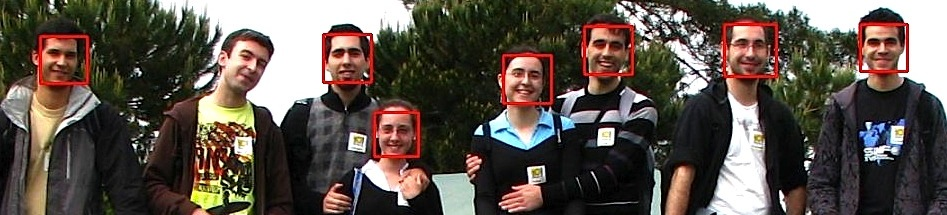
\includegraphics[width=\columnwidth]{Figures/faces1.jpg}
	\caption{Example of the OpenCV library detecting faces on a common photo.}
	\label{fig:faces1}
\end{figure}

No face recognition software is perfect. Usually if the software can detect every face, it will probably detect some other things in images that aren't faces (false positives). If it’s successful in only detecting faces, it will probably miss some other faces that aren't ideally positioned (false negatives). OpenCV is included in the latter, only detecting faces but also missing some that are tilted (like in \fig{faces1}) or turned on the side.


This process is quite computationally expensive and therefore we resize all the images down to a more acceptable size, making the process more than five times faster.

We tested 29 images, from six different cameras, ranging from one to ten megapixels, and containing up to thirteen faces. The test consisted in running face detection on each image, in its original size and in various resolutions from 2000 to 200 pixels on its longer side, comparing the number of faces recognised and the time needed to process them. The results can be seen in \fig{fdres}.

\begin{figure}[ht]
	\centering
		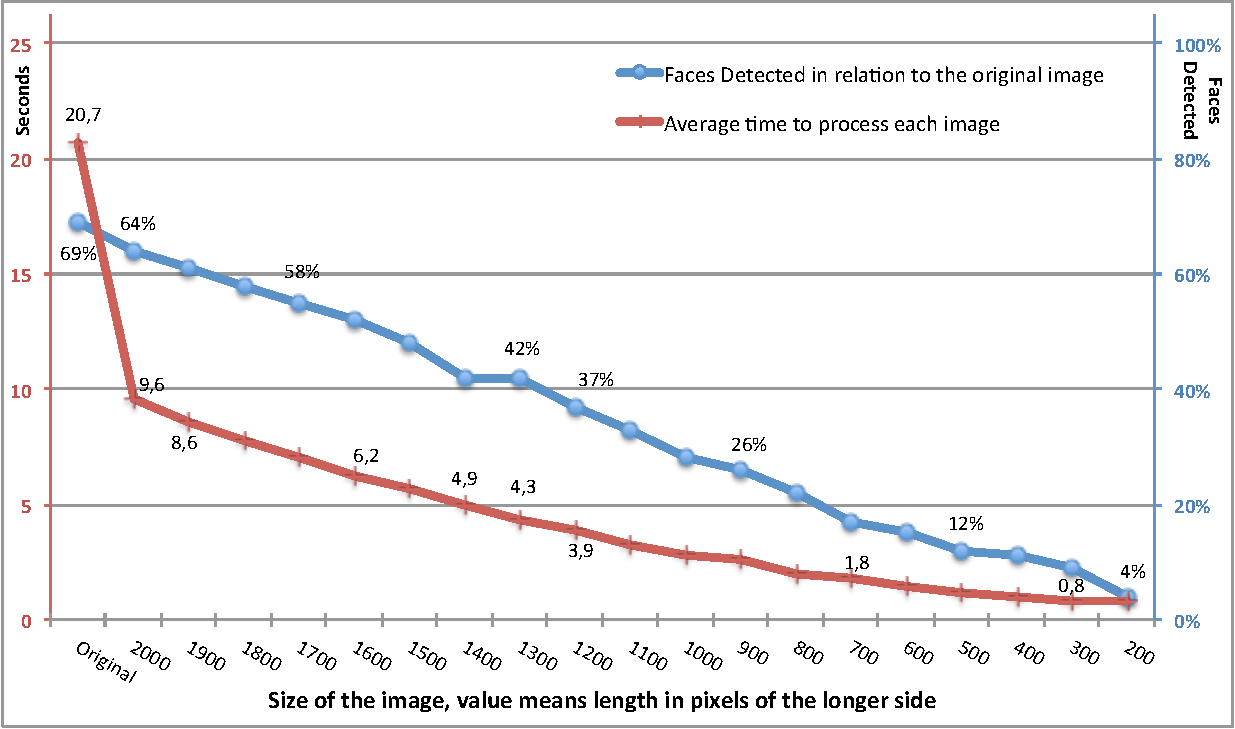
\includegraphics[width=\columnwidth]{Figures/graph2.pdf}
	\caption{Results of the face detection test. 100\% of faces is the actual faces present in the test images.}
	\label{fig:fdres}
\end{figure}

The purpose of this test is to identify how much can we reduce the images while maintaining a high recognition rate, we are comparing the recognition results of the downscaled versions to the original size and analyze the speedups and failures in recognition. We do include the number of faces actually present in the photos for comparison, corresponding to the 100\% value in \fig{fdres}.

We can see that by only reducing the images to 2000 pixels on the longer side, the processing time fell to less than half (20.7 to 9.6) without much loss in recognition (69\% to 64\%). The 1300 pixels was the chosen value for being the last with more than 40\% recognition rate (60\% of the full size image) and being 4.8 times faster\footnote{4.3 seconds per image versus 20.7; one hour and 10 minutes per thousand images versus almost six hours} than using the original image. In the future, with more tests, we can fine tune the resizing algorithm to get better results.



\hide{ver que caras falham primeiro para perceber o que aconteceu. As caras que se perdem são relevantes?}
% subsubsection face_detection (end)


\subsubsection{Generation of multi-scale imagery}

This plugin generates all the data files needed for the visualization to work. As referred previously, the visualization relies on the DeepZoom technology and it needs to process the images before they can be displayed. This plugin does exactly that.


Using a library from Microsoft, the plugin generates, for each image, a metadata file and a set of image files representing the original one at multiple scales, from a single pixel to a large, detailed image.

After passing through all images, the collection as a whole is subject of additional computation, this time generating imagery for all images as a single set and a metadata file that agglomerates all image sets used. This metadata file for the collection (called collection.xml) is then altered by the plugin to attach to each image, the data previously generated by the other plugins.

% subsection plugins (end)


\section{Visualization} % (fold)
\label{sub:visualization}

As referred on \ref{sub:design_decisions} we built the visualization with Silverlight and DeepZoom. It runs inside a browser window which can make a very immersive experience when put in fullscreen.

The system loads the DeepZoom files and the 


% subsection visualization (end)










\cleardoublepage

\chapter{Evaluation} % (fold)
\label{chapter:evaluation}

% 10/15 pages

To better understand how well Eagle Eye works, we performed user testing and, to do that, we defined a number of goals for Eagle Eye and a testing methodology, with specific tasks to be performed by the users. We also did separate tests with the users' own libraries to evaluate the benefits of knowing the contents of the system.





\section{Objectives}

With our tests, we wanted to observe how various parts of Eagle Eye worked for a variety of people. 
We will answer the following questions, with our evaluation of the system:

\begin{itemize}
\item How the users react to the large quantity of images displayed simultaneously?
\item How easily do the users understand how to use the navigation controls and what could be improved?
\item Do users think the available disposition and sorting options are adequate and useful?
\item Can users understand what are the filters capable of, or there is a need for an improvement?
\item Can users extract interesting information from the collections by using Eagle Eye?
\end{itemize}

The answers will be provided later on, after explaining the testing and the results.




\section{Testing Methodology}

We performed two different tests with users, both with different purposes.

One of the tests is the ideal use-case for our application: the scenario where the users are interacting with their own photos through our system. A few users gave us their photo libraries for us to process, so that we could test the usage of the user's own library in Eagle Eye.

The other test we performed allowed us to broadly analyze how users responded to the \ac{UI}, how they interacted with the system, how long some tasks took to complete or how did they chose to perform a certain task. This test only makes sense if we can replicate the conditions for each user so we generated a fixed collection, equal for all users who performed this test. This collection had 5679 photos and was based on a subset of my own photo collection, with images spanning from 2005 up to 2011. We had a larger number of users perform this test, for more accurate quantitative results.

Testing was done by presenting the user with the Eagle Eye's visualization interface ready to use. They never saw the backend or any of its processing steps, since that part is currently less then polished, takes a long time to process, and is not what we are interested on testing.

The interface and controls were explained in detail to the users, from how to navigate the collection to the functions of the buttons on the \ac{UI}. They were then allowed to play around, explore and learn Eagle Eye by themselves. I was always next to them, giving little hints and some occasional help. After they felt comfortable with the system, I asked them to perform a few tasks, measured time and errors and in the end asked them to answer a few questions, describing what they thought of the system.

Most tests where performed on my personal laptop computer, connected to a 22" external monitor. The big screen is very important and helps provide a better experience while using Eagle Eye, for its capacity to display the images in a larger and more comfortable size than my 13" screen computer. Other tests had to be performed directly on the laptop, since I had to meet some users at their work locations on the university campus.





\section{Characterization of users}

We tested 18 people, 16 of them students in this institution, between the ages of 21 and 25, from the various degrees of computer engineering. The rest were composed from people between 40 and 55 years.

Nine of our users said they took photography seriously, although not professionally. Eight said they just like to take pictures for keeping memories or just used their camera phone and the other person doesn't take pictures (\fig{chart:photographers}).

Ten people claim to have less than 5000 photos stored on their computer, two people said they had between 5 000 and 10 000 while the other eight people that more than 10 000 photos (\fig{chart:libsize}).

From the 18 users, only the user that doesn't take pictures relied exclusively on the organization provided by an application, while all others keep their photos on folders, some using applications to help manage them. The applications in use can be seen in \fig{chart:apps}. Additionally, all users except one have a systematic way to organize their collections, being them inside an app or not.

\begin{figure}[!htb]
  \begin{subfigmatrix}{3}
    \subfigure[How users see themselves as photographers.] {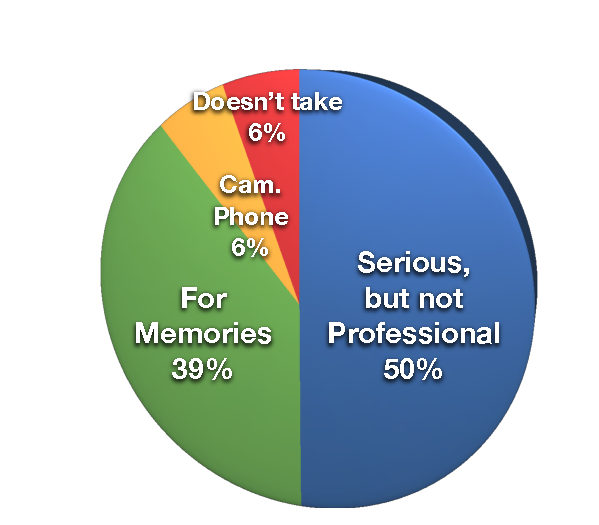
\includegraphics[width=0.3\linewidth]{Figures/charts/photographers.pdf}\label{fig:chart:photographers}}
    \subfigure[Size of users' photo library.]{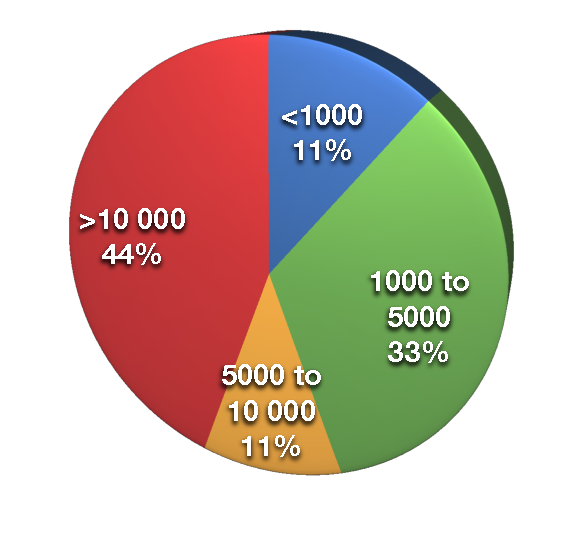
\includegraphics[width=0.3\linewidth]{Figures/charts/lib-size.pdf}\label{fig:chart:libsize}}
    \subfigure[What they use for organization.]{\includegraphics[width=0.3\linewidth]{Figures/charts/software.pdf}\label{fig:chart:apps}}
  \end{subfigmatrix}
  \caption{User characterization.}
  \label{fig:linear}
\end{figure}




\section{Test Results}

We will now go through the results of the testing, starting with the behaviors of the users during the process of learning to use Eagle Eye. After that, users were asked to perform some tasks and we will see some of the more interesting parts of that process, followed by the most common errors and problems faced by the users. After the test, we asked the users to answer a inquiry and its results will be detailed towards the end of this section.


\hide{The general feedback obtained is that users generally like the concept and the interaction of the system. They like to explore the library in different ways and play around with the dispositions. The majority have concluded that it needs some improvements in certain areas.}




\subsection{User behavior during exploration}

Upon being told how the system worked, users generally went ahead and played a while with the zooming, and viewed some images and groups at will, while noticing how the groups can be differentiated when zoomed out.

Next, users tried the different disposition options, generally in the order they are presented in the \ac{UI}. The motif for two date displays was usually questioned and, after an explanation, they move on to the color display which they usually liked for the nice and clear color separation, although, when viewed more closely, some images appeared in odd locations.

After understanding the differences in dispositions and viewing some groups/images more zoomed in, the users tried the filtering or the manual selections for reducing the amount of images displayed and focus only on part of the collection. The filter showed useful even though its bugs occasionally made an appearance. The manual selections were easier to use and for that captivated more usage from the users.





\subsection{Results for tasks}

After playing around with Eagle Eye, we asked the users to perform some tasks for us. We measured how long did they take to do each task and what errors they've done. Bellow the description of the tasks are graphs (figs. \ref{fig:tasks:graph:time} and \ref{fig:tasks:graph:errors}) with a summary of the measurements.

We started with simple tasks, to see if they understood the basics of the system. Tasks like ``Switch to the color view'', ``Select and display a group'', ``Select and display a few images'' weren't problematic and generally took between a couple seconds up to about 15 seconds, depending on the user, and without errors. We also asked for a simple combination of functions with the task ``what is the most common color of the pictures taken with the most used camera?'', which is the process of sorting by camera, selecting a group and sorting by color. 18 people finished the test in less than half a minute without problems, the other two made one mistake 

Next, we asked users to select images from the year 2010. This could be done by using the filter to only display images of that year or by viewing images by sequential date and manually select the images that corresponded to that year. Most users tried typing 2010 in the filter bar and quickly got to the intended result in about 5 seconds, but four users still looked into the default, treemap-based, date view until they remembered/noticed it wasn't sorted and then looked for the sequential date view and performed a manual selection of the images. These users took about a minute to perform the operation.

In another test, we told the users that the library had photos of a certain annual event and asked them to figure out what years had photos of that event. The easier way was to filter by the event name, sort by date and view the group names, which would take less than 15 seconds. Slightly more than half the users did this method. Others went to the path view and looked for groups containing the event name, taking between one and two minutes to perform the task. A small percentage tried to discover the photos by navigating on the complete image set, taking an even longer time to complete.


\begin{figure}[p]
	\centering
		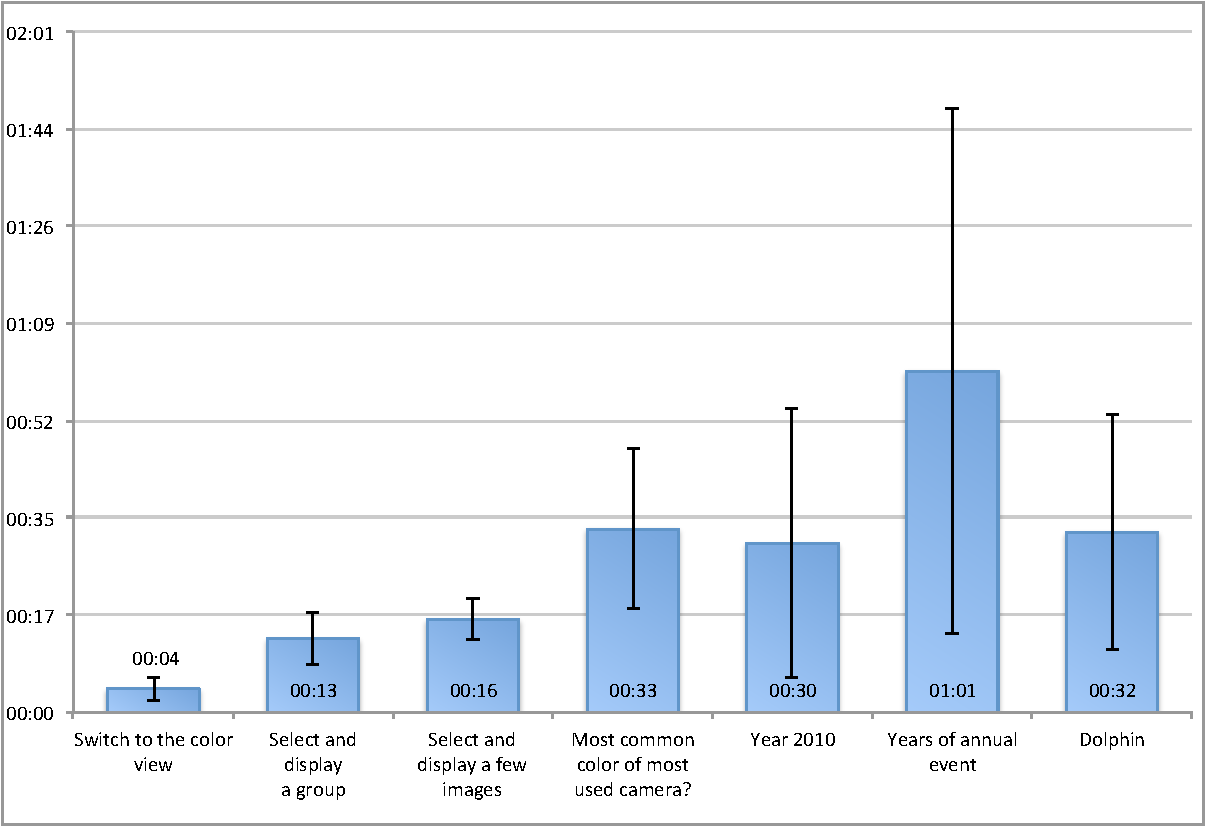
\includegraphics[width=0.9\linewidth]{Figures/tasks-graphs-time}
	\caption[Graph of time spent on each task]{Time (average and standard deviation) spent by users for each of the tasks.}
	\label{fig:tasks:graph:time}
\end{figure}

\begin{figure}[p]
	\centering
		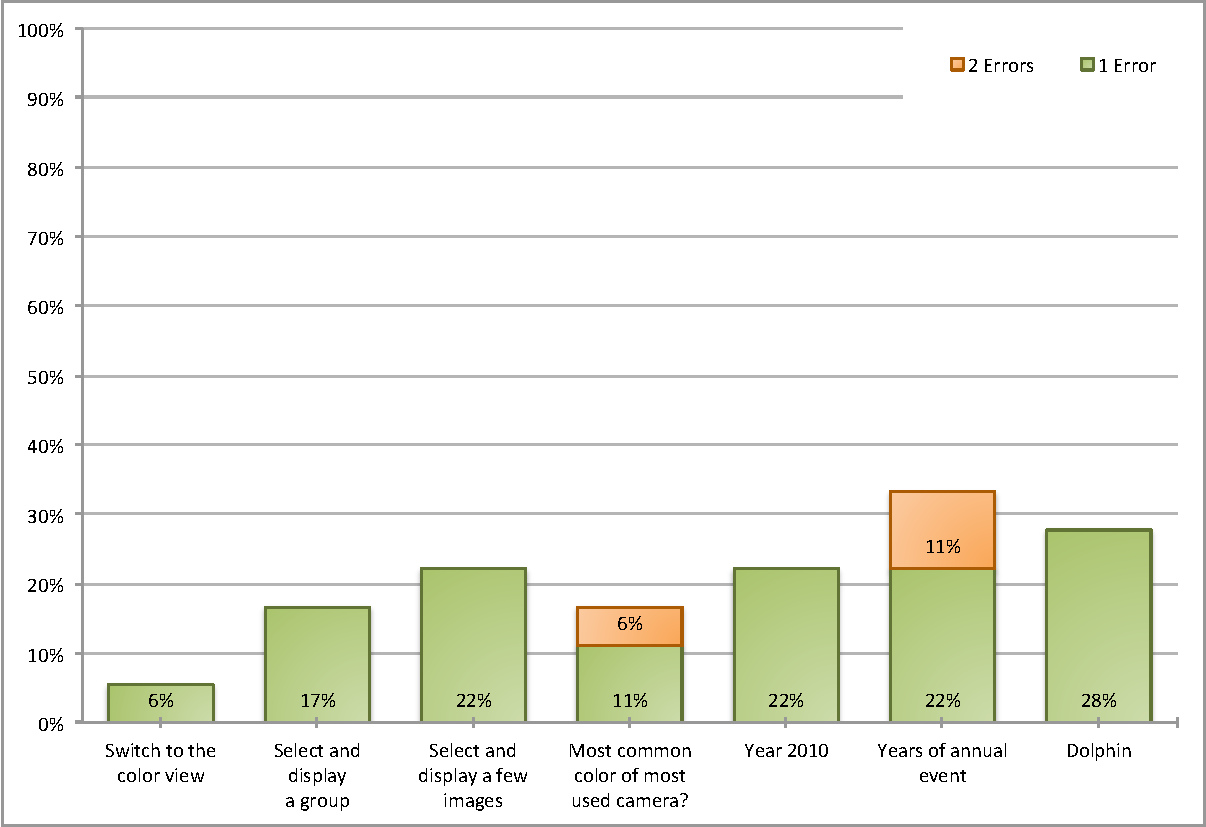
\includegraphics[width=0.9\linewidth]{Figures/tasks-graphs-errors}
	\caption[Graph of errors made on each task]{Percentage of users who made errors on each task, grouped by how many errors.}
	\label{fig:tasks:graph:errors}
\end{figure}

The users were then asked to find a photo of a jumping dolphin. This test could be accomplished in variety of ways. Some users had already noticed a group of photos of the Zoo and zoomed into those, quickly finding the photos in less than ten seconds. Others changed the view to be grouped by colors and selected only the blue groups. The filter returned the photos in no apparent order and, after complaining about that, the users changed the view to date or path, finding the group of Zoo photos on the corner. Some zoomed in, others selected that group and found the photos, not taking less than 30 seconds to do it. A few users tried at first to see if there were some dolphin-related keywords but, unfortunately, those photos had no keywords associated.








\subsection{Errors and misunderstandings} % (fold)

During the above two tests, exploration and tasks, some errors occurred somewhat repeatedly, some caused by bugs, some by poor choices in the \ac{UI}.

Users could not quickly understand the difference between the buttons ``Date'' and ``Date (Linear)'' buttons by themselves making some mistakes sometimes.

A few users though the ``Select images'' button was for applying the filters and not for manually selecting images, generating some confusion.

A few other users complained about the way to manually select a single image. Currently, the user is required to make a ``click-and-drag'' selection to select one or multiple images, conflicting with the common way of ``click to select item; click-and-drag to select many''.

Another problem, detected by a few users, that is also related to selections is the action of de-selecting images and groups, which can only be performed by deleting the entry in the filter bar, and not by interacting with the images.  





\subsection{System Usability Scale}

On the inquiry filled by our test users after the testing the system, we had a section with the \acf{SUS} questions. \ac{SUS}\cite{Brooke:1996ua} is a simple and generic ten question scale, giving a global view of the usability of a system. The \ac{SUS} result of inquiring 18 people was 75 points\footnote{With a standard deviation of 9 and a median of 75.} on a scale of 0-100 points, which is a fairly good mark for our system. With the missing improvements it could score higher.

The averaged results to each of the answers of \ac{SUS} can be seen on Table \ref{tab:sus}. The questions' focus alternates between positive and negative characteristics for the system. Some important questions got good rates, like the ``easy to use'' and ``quick to learn'' with ratings of 4.3 and 3.9 of a maximum 5 and the ``unnecessarily complex'' question also getting the second best rate for a negative question, 1.6, which means users generally found the system to be easy to use and learn, although it still has some margin for improvement on the user experience area. Another important question is the ``I would like to use this system frequently'' which got a rating of 3.4, slightly lower from what we would like to see but still above the waterline. We tried to understand if the kind of photography or the size of the library had an influence on this value but we got mixed results and concluded that they probably aren't connected. Even though, this rating reinforces the point above about the need for improving the system, but this time by adding features that could make the user want to use the system more often.

\vspace{\baselineskip}

\begin{table}[h!]
	\rowcolors{0}{light-gray}{white}
	\renewcommand{\arraystretch}{1.5}
	\centering
\begin{tabular}{l|c}
I think that I would like to \textbf{use this system frequently} & 3.4\\
I found the system \textbf{unnecessarily complex} & 1.6\\
I thought the system was \textbf{easy to use} & 4.3\\
I think that I would \textbf{need the support of a technical person} to be able to use this system & 1.6\\
I found the various functions in this system were \textbf{well integrated} & 3.5\\
I thought there was \textbf{too much inconsistency} in this system & 1.9\\
I would imagine that most people would \textbf{learn to use this system very quickly} & 3.9\\
I found the system very \textbf{cumbersome} to use & 1.9\\
I felt very \textbf{confident} using the system & 3.7\\
I needed to \textbf{learn a lot of things} before I could get going with this system & 1.5\\
\end{tabular}
\caption[Average of the results for each of the ten questions of \ac{SUS}.]{Average of the results for each of the ten questions of \ac{SUS}. Values range between 1.0 (strongly disagree with the question) and 5.0 (strongly agree). Gray rows are ``positive'' questions, where higher values are better, and white rows are ``negative'' questions, where lower values are better.}
\label{tab:sus}
\vspace{\baselineskip}
\end{table}





\subsection{What users liked}

Questioned of what they liked on the system, and from what was seen from the interaction, we can confidently say users liked the general concepts of the system. I now present a summary of the users opinions of the good points of Eagle Eye:

\pagebreak

\begin{myitemize}
\item It was easy and simple and it helps to get a good overview of the photo collection;
\item the photo display of a much greater amount of photos than what they've ever seen, making visualization of many images easier;
\item the easy zoom in and out to quickly see groups or photos in full size or in smaller size;
\item still being able to identify groups of images which are small sized;
\item the intersection of filters/groups, i.e., the various ways to quickly organize and access the images, specially the ability to view groups by events or colors;
\item the ability to select images;
\item the smart use of space by grouping related images;
\end{myitemize}

Essentially, people seem to like the new interaction methods to browse photos, specially if they know the photos themselves, which makes the overall usage of the system much more interesting.




\subsection{User suggested improvements}

During the course of the tests and on the questionnaire, some users suggested some improvements to our work. Some of these improvements were already in our mind but we didn't had enough time to implement them. We will now expose the suggestions we agree on:

\begin{myitemize}
	\item Information to help the user use the system, e.g., help, guides or tutorial;
	\item When there's many images, display a few from each group in a bigger size and on zoom in, display more;
	\item Easier way to quickly view a single image/group in full size, like a double click;
	\item The filter should the improved, removing the bugs, giving some guidance to the user and allowing both \texttt{AND} and \texttt{OR} logics (currently only uses the former) and a button to clear it;
	\item The selection buttons should be separated from the filter bar to avoid misleading people;
	\item The display should be organized hierarchically where appropriate, e.g., date, path and color based visualizations;
	\item The color measure should be improved;
	\item Event-based visualization, better then just dates or paths;
	\item Face detection should be improved to Person recognition;
	\item Improved method to select single images;
	\item Display the number of photos on screen;
	\item Better group separation.
\end{myitemize}

Although we tried to make the user interface as clean and simple as possible, a couple users found some difficulties and suggested some simple guides. We think a simple introduction to the system is nice and helps the users, but it wouldn't make sense to spend time doing it at this point.

\pagebreak




\section{Accomplished Objectives} 

We can now answer what objectives for Eagle Eye were accomplished. 




\subsubsection{How the users react to the large quantity of images displayed simultaneously?}
Users generally liked the large view and were surprised by how much can still be recognized, specially when working with their own photos and if they're grouped by events. 




\subsubsection{How easily do the users understand how to use the navigation controls and what could be improved?}
Users like the navigation controls but many felt it should be easier to go directly to a full view of one image and some agreed that keyboard navigation or slideshow-like controls should make the navigation easier.




\subsubsection{Do users think the available disposition and sorting options are adequate and useful?}
Users liked the ability to switch between dispositions and preferred some more the others.
Users generally liked the date display in groups but some would prefer that it would be more faithful to the time. Some suggested that it would be better if the tree map was organized with groups and subgroups so that all photos of a year/month got grouped together. Users understood the current need for the linear date display but found it hard to view anything and didn't spend much time with it.
The other preferred disposition was the color, the overall result of the grouping was pleasing to the eye of most users. The problem was when they started zooming in and some images revealed to be a mix of different colors from the color of the group they were in. This was a known problem of the method used. Another problem that revealed was the large size of groups like ``Gray'' or ``Black'' usually took great part of the screen, leaving all the more interesting colors to half of the screen. Some users even filtered out this black and grey groups by selecting and viewing only the colorful ones.
The path display wasn't very used since it ended up being much similar to the date display, except on some libraries where there folders weren't named by date but by event and made some sense to view the groups by these names. 




\subsubsection{Can users understand what are the filters capable of, or there is a need for an improvement?}
Some users understand what the filter is capable of when the autocomplete gives some suggestions, others could use some initial guidance to understand that a lot of things can be used on it. The biggest problem is that some of the information they would like to use can't be obtained automatically, like location (unless already on EXIF) or names of people, unless we hook into some third party app where the user have previously saved this data.




\subsubsection{Can users extract interesting information from the collections by using Eagle Eye?}

Users can extract some information about their collections, like collection sizes, days with many shots, most common colors, most common devices and such. It would be even more useful with the inclusion of a second grouping and sorting option so, for instance, a disposition by devices could have the images inside each camera sorted by their color. This way even more information could be retrieved from the collection.





\section{Case Studies}

As referred on the beginning of the chapter, we made some tests with some users' photo collections. We managed to get five users willing to to give us a copy of their collections for a more personalized testing.

We got libraries containing from 833 up to 6064 images. None of the tested users  Most users report being able to recognize most of the  groups in Date view. The user with the most photos said he needed to zoom in a little to understand better some of the groups, since many of them had a similar, grayish, tone that made them a bit hard to distinguish. We experimented filtering out all the images in the gray category using the color view and get back to the date view and groups were much easier to distinguish, because there were a lot of less images to view, making the visible ones bigger, and because groups had now a more relevant color. Although we were hiding images, the view itself ended up more interesting.

\begin{wrapfigure}{r}{0.45\textwidth}
	\vspace{-20pt}
	\begin{center}
		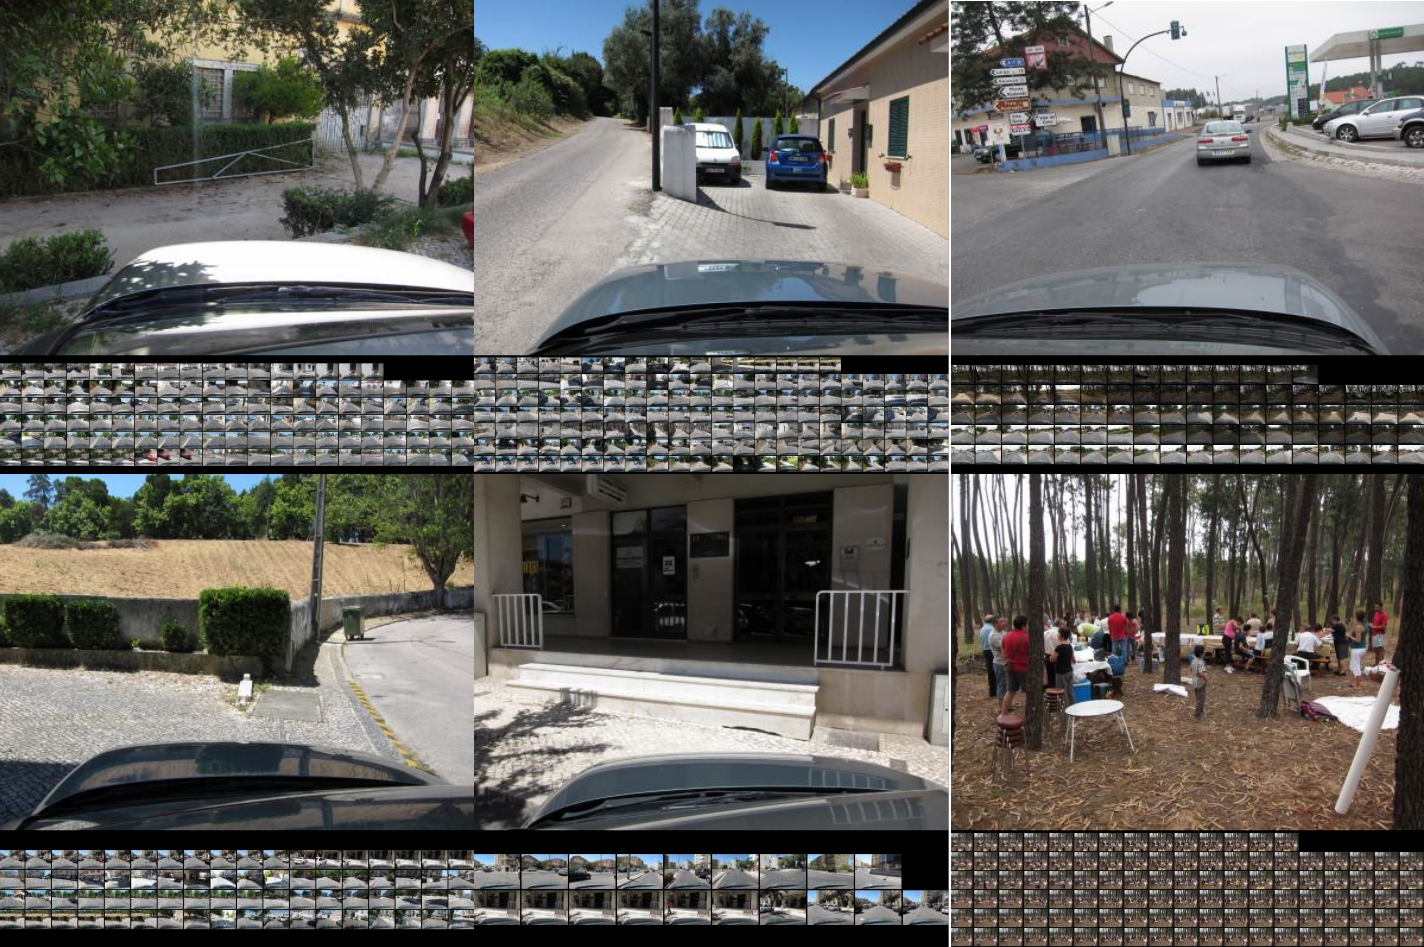
\includegraphics[width=\linewidth]{Figures/filcab-time-lapse-563-imgs-to-6.png}
	\end{center}
	\vspace{-20pt}
	\caption{Case study: six time lapses of 563 images, reduced to 6 spaces on the canvas}
	\vspace{-5pt}
	\label{fig:filcab:stacks}
\end{wrapfigure}

Most tested users only had a couple images stacked and did not use any of the techniques that produced sequential images (e.g. panoramas, bracketing, burst) but the person with the biggest library did made some bursts and some long time lapses and most were correctly stacked. This stacking allowed his collection of over 6000 photos to fit on the space occupied be a collection of only 4368 images, which is a 27\% reduction of clutter, without actually hiding the images. As an example, specific to this library, we selected the largest stacks on his library and compared how much space they took compacted and expanded. The six stacks we chose (\fig{filcab:stacks}) contained, in total, 563 images. By stacking, the 563 very identical images took only the space of 6, which is about 1\% of the space. We know that not many people make this type of photography but, for those who do, stacking is a very helpful feature which can only be improved.






\section{Discussion}

With the tests we performed, we verified people generally liked Eagle Eye and saw the potential of the system.

We designed it to be simple while powerful, and people proved it was simple, by their positive answers and by their usage of the system, where we not only measured generally low times to complete the tasks but also a low number of errors. We acknowledged some aspects of the interface could be improved for a better and more user-friendly interaction.

By the user interactions and suggestions, we also understood that Eagle Eye could be even more powerful, and with some improvements on the extraction of features and by enhancing the capabilities of the organization on canvas, it could be much more interesting and relevant to anyone who keeps photos on their computer.

%%%%%%%%%%%%%%%%%%%%%%%%%%%%%%%%%%%%%%%%%%%%%%%%%%%%%%%%%%%%%%%%%%%%%%%%
%                                                                      %
%     File: Thesis_Conclusions.tex                                     %
%     Tex Master: Thesis.tex                                           %
%                                                                      %
%     Author: Andre C. Marta                                           %
%     Last modified : 21 Jan 2011                                      %
%                                                                      %
%%%%%%%%%%%%%%%%%%%%%%%%%%%%%%%%%%%%%%%%%%%%%%%%%%%%%%%%%%%%%%%%%%%%%%%%

\chapter{Conclusions}
\label{chapter:conclusions}

% 3/4 pages

Insert your chapter material here...


% ----------------------------------------------------------------------
\section{Achievements}
\label{section:achievements}

The major achievements of the present work...


% ----------------------------------------------------------------------
\section{Future Work}
\label{section:future}

During the realization of this work, many ideas popped in our minds but we didn't had the time to work on them.

The most important effort that must be done to this work is a rearrangement of the backend and its connection to the visualization. As we've seen on chapter \ref{cha:eagle_eye}, both parts of this work are currently separated and the backend is a command line utility. Our idea was to create an graphical application where the user could enter the folder paths he want's added to Eagle Eye and then the application would do the needed work on the background, using free resources, and when it was done, the user could enter in the visualization mode without the need to open a browser window.

The second important thing to do is to improve the feature extraction plugins. The color plugin, for instance should be able to better identify colors in images instead of simply make an average. More data should also be extracted from the EXIF, for instance, location data should be translated into place names\footnote{The action of turning GPS coordinates into addresses is called reverse geocoding. An example of a provider of such service: \url{http://code.google.com/apis/maps/documentation/geocoding/index.html\#ReverseGeocoding}}

On the visualization part, the linear disposition, used mainly by the date view, should be improved to make more clear the distinction between days, months, years. Another idea for a different disposition born from the stacking of similar photos discussed in section \ref{ss:stacks}, where one image is bigger than the rest, to help identify what is on what group.

To conclude, we think it needs to be more slideshow friendly, so that by the press of a button on the \ac{UI} or on the keyboard, a sequence of images could be viewed in fullscreen without having to drag and drop the canvas between each image. 

In our view, Eagle Eye would be a useful photo viewer that could be used by anyone that has some computer knowledge and a photo database on the computer.

\cleardoublepage



% ----------------------------------------------------------------------
%  Appendix (optional)
% ----------------------------------------------------------------------
%\appendix
%%%%%%%%%%%%%%%%%%%%%%%%%%%%%%%%%%%%%%%%%%%%%%%%%%%%%%%%%%%%%%%%%%%%%%%%%
%                                                                      %
%     File: Thesis_Appendix.tex                                        %
%     Tex Master: Thesis.tex                                           %
%                                                                      %
%     Author: Andre C. Marta                                           %
%     Last modified : 21 Jan 2011                                      %
%                                                                      %
%%%%%%%%%%%%%%%%%%%%%%%%%%%%%%%%%%%%%%%%%%%%%%%%%%%%%%%%%%%%%%%%%%%%%%%%

\chapter{User Survey}
\label{appendix:usersurvey}

We asked some people to answer a survey and we got 30 answers that helped us understand photography related habits and user wishes, and compiled them in this appendix.

\section{User characterization}

Our survey started by asking the respondents to describe themselves and their libraries.


\subsubsection{Kind of Photographer} % (fold)
\label{ssub:subsubsection_name}


\begin{wrapfigure}{r}{0.3\textwidth}
	\vspace{-20pt}
	\begin{center}
		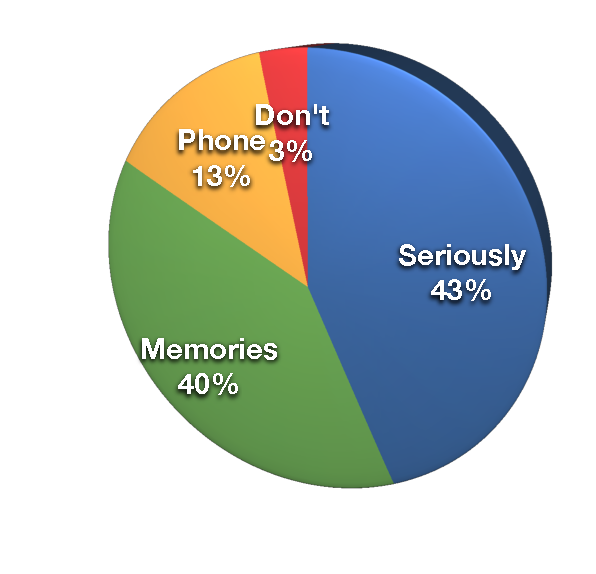
\includegraphics[width=\linewidth]{Figures/survey/desc}
	\end{center}
	\vspace{-20pt}
	\caption{Kinds of photographers.}
	\vspace{-5pt}
	\label{fig:us:desc}
\end{wrapfigure}

We asked the respondents what of the following options described them the best:

\begin{myitemize}
	\item I'm a \textbf{professional} photographer.
	\item I like to take photography \textbf{seriously} but I'm no professional.
	\item I like to take pictures just to keep as \textbf{memories}, but I'm not a photo-geek.
	\item I only use my camera \textbf{phone} for fun.
	\item I \textbf{don't} take pictures.
\end{myitemize}

As we can see on \fig{us:desc}, most respondents like photography and take photos, being mostly people who take photos for memories and people who are really into photography but are not professionals.

% subsubsection subsubsection_name (end)





\subsubsection{Storage of digital photos} % (fold)
\label{ssub:storage_of_digital_photos}
The second question was a check to verify if the respondents stored digital photos in their computers. The questionnaire would end if they said no. Fortunately, everyone said yes.
% subsubsection storage_of_digital_photos (end)





\section{Characterization of Photo Library} % (fold)
\label{sec:characterization_of_photo_library}

\begin{wrapfigure}{r}{0.5\textwidth}
	\vspace{-20pt}
	\begin{center}
		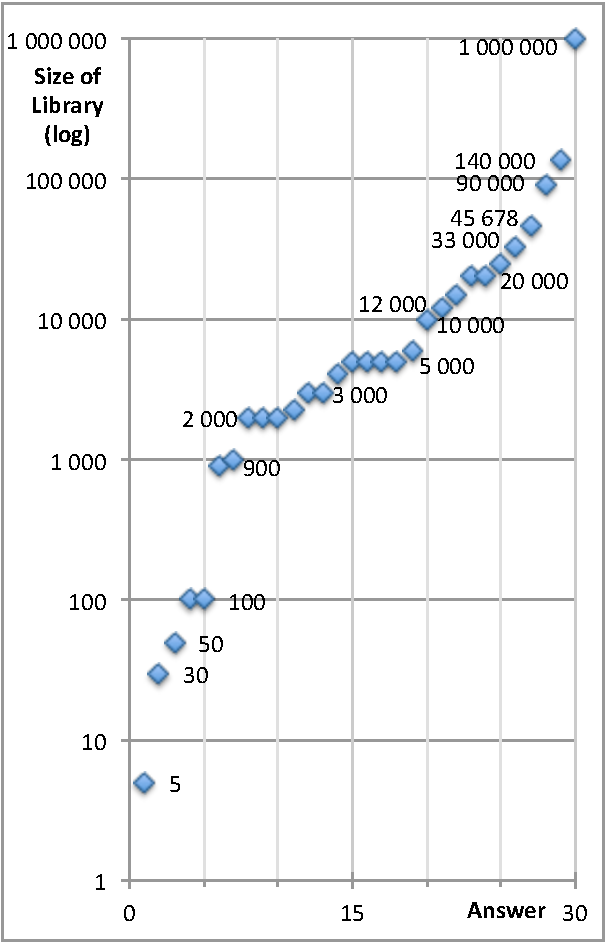
\includegraphics[width=\linewidth]{Figures/survey/libsize}
	\end{center}
	\vspace{-20pt}
	\caption{Library Size}
	\vspace{-70pt}
	\label{fig:us:desc}
\end{wrapfigure}

We then inquired about their photo libraries.
\vspace{\baselineskip}

\subsubsection{Library size} % (fold)
\label{ssub:library_size}

To start the survey about the library, we inquired how large was the respondents photo library.

We made this an open question, because we wanted to obtain real values from the users and not just limiting to a number of options that hardly represent anything. The answers for this question can be seen on \fig{us:desc}.

We were surprised by the values we got, going from 5 up to a million photos.

Almost half of the answers are between the 1 \nolinebreak 000 and the 10 000 values, having two thirds of the results falling between 0 and 10 000. We also found the median value of the answers, which is 5 \nolinebreak 000.

% subsubsection library_size (end)


\vspace{3\baselineskip}

\begin{wrapfigure}{r}{0.3\textwidth}
	\vspace{-20pt}
	\begin{center}
		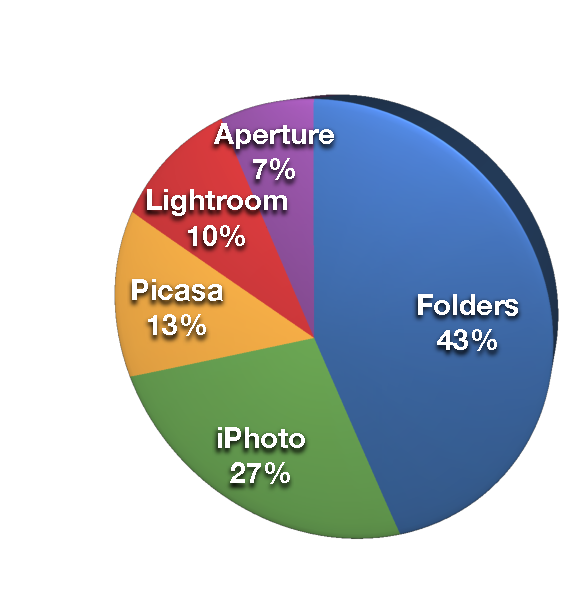
\includegraphics[width=\linewidth]{Figures/survey/sw}
	\end{center}
	\vspace{-20pt}
	\caption{Software used}
	\vspace{-5pt}
	\label{fig:us:desc}
\end{wrapfigure}

\subsubsection{Usage of Software} % (fold)
\label{ssub:usage_of_software}

We then questioned about what software applications did people use to help them organize their collections. Almost half admitted they only used folders for their organization, while the other 17 people used some kind of software.

Going through each software applications, we can see that 40\% use an entry-level software (iPhoto and Picasa) while 17\% prefer more Pro-level systems.

We tried to correlate the size of the collections with the software used but we realized that we probably don't have enough data for some of those softwares and that users might not have their entire collection inside the application, therefore defeating the correlation.

% subsubsection usage_of_software (end)

\pagebreak


\subsubsection{Systematic Organization} % (fold)
\label{ssub:systematic_organization}

\begin{wrapfigure}{r}{0.25\textwidth}
	\vspace{-20pt}
	\begin{center}
		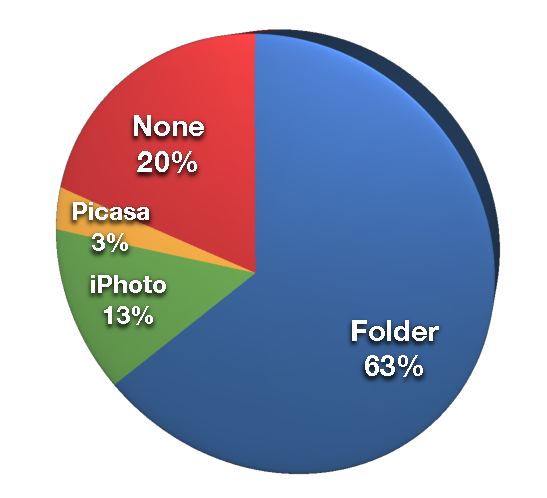
\includegraphics[width=\linewidth]{Figures/survey/organization}
	\end{center}
	\vspace{-20pt}
	\caption{Systematic organization in folders, in an application or no organization.}
	\vspace{-5pt}
	\label{fig:us:org}
\end{wrapfigure}

The question ``Do you have a systematic way to keep your photos organized?'' is meant to understand if people keep a system for their library, either on folders of inside an application.

Since most of the applications in the last question rely on folder organization, is no surprise that having a system in place for keeping things organized in folders is the clear winner of this question. Five people answered that they have this system inside an application and correlating this question with the previous one we found another expected aspect: only entry-level software is used to keep everything tidy, without touching folders, more exactly four people say they use iPhoto and one says Picasa is his/her choice.

In contrast, 20\% of the respondents claimed not having a way to organize their collections. The median of the number of photos of this group of people is 1050, the lowest, when compared to the other groups, the ones who use applications and the ones who rely on folders, both with 5000 of median.

% subsubsection systematic_organization (end)



\subsubsection{Photos in Close Sequence} % (fold)
\label{ssub:photos_in_close_sequence}

\begin{wrapfigure}{r}{0.25\textwidth}
	\vspace{-50pt}
	\begin{center}
		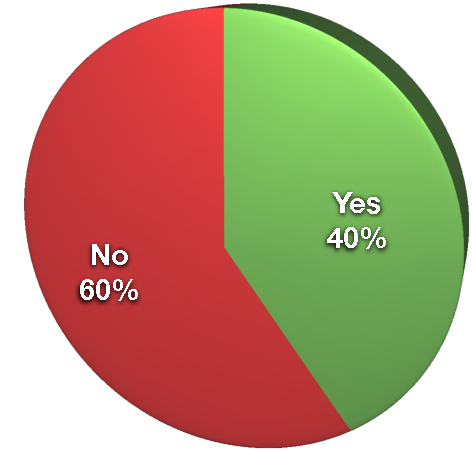
\includegraphics[width=\linewidth]{Figures/survey/close-seq}
	\end{center}
	\vspace{-20pt}
	\caption{Users that take photos in close sequence.}
	\vspace{-5pt}
	\label{fig:us:close-seq}
\end{wrapfigure}


% subsubsection photos_in_close_sequence (end)

The following question was intended to see how many users take photos in close sequence, e.g., bursts, panoramas, bracketing or time lapses, where the photographer ends up with many photos in a few seconds.

As we can see on \fig{us:close-seq}, 40\% of the respondents said they do take photos in close sequence. We also saw that this group has a median value of library size of 8000, whereas the other group stays on the 2150 images. In fact, of the total 13 enthusiasts, 11 of them answered yes on this question, followed by someone who claims only to take photos for memories.



\subsubsection{Preferred Features} % (fold)
\label{ssub:preferred_features}

\begin{wrapfigure}{r}{0.45\textwidth}
	\vspace{-50pt}
	\begin{center}
		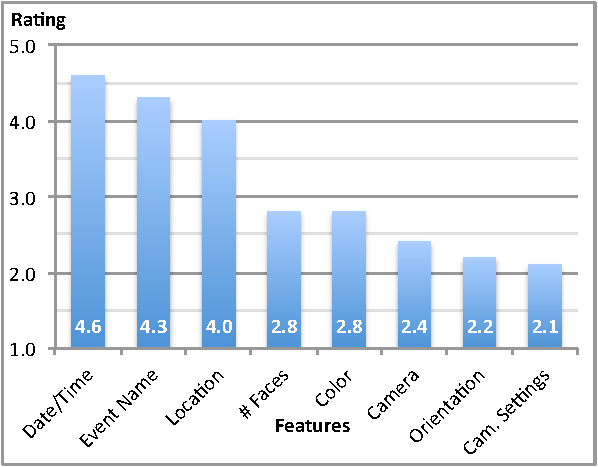
\includegraphics[width=\linewidth]{Figures/survey/features}
	\end{center}
	\vspace{-20pt}
	\caption{User rated features.}
	\vspace{-5pt}
	\label{fig:us:features}
\end{wrapfigure}

We had some ideas of what we would like to see extracted from the images and exposed to the user via our application and we asked for people's opinion on this survey and the results can be seen on \fig{us:features}.

While we weren't surprised by the favorites\linebreak Date/Time, Event and Location, we did expect\linebreak some higher ratings for number of faces and colors. Orientation and camera settings got the ratings we did expect.

% subsubsection preferred_features (end)



\subsubsection{Suggestions of Features} % (fold)
\label{ssub:suggestions_of_features}

In line with the previous question, we asked what other features they would like to see extracted from images.

\begin{itemize}
	\item The most common request, with about four different people requesting it, is people recognition. This allows photos to be tagged with the names of people in the photo and not just how many faces there are on the photo.

	\item Someone asked that, from a set of similar photos (exemplified with friend group photos), pick the one that, e.g., is more clear, has a better color, more smiles, more open eyes.

	\item Metadata was requested by three people, e.g., EXIF metadata, tags, format (RAW/JPEG), if the photo is the original or the edited version, the number of duplicates, the location on disk.

	\item One person asked for identification of whether the photo was taken during the day or the night.

	\item Another person was interested in having information about objects, buildings or animals.
\end{itemize}


\subsubsection{General Overview} % (fold)
\label{ssub:general_overview}

\begin{wrapfigure}{r}{0.4\textwidth}
	\vspace{-20pt}
	\begin{center}
		\includegraphics[width=\linewidth]{Figures/survey/overview}
	\end{center}
	\vspace{-20pt}
	\caption{Whether people think they can get a good overview or not.}
	\vspace{-5pt}
	\label{fig:us:overview}
\end{wrapfigure}

To conclude the survey, we asked if the respondents feel they have the tools to have a good overview of their collection at the same time.

The answers to this question rose some uncertainty, due to their mixed views. Each person is different from the next and so are their requirements. For instance, some people considered iPhoto/Apertures's events or projects as good overview for the library, but others don't think the same way about it, claiming it is limiting. On \fig{us:overview}, is a summary of whether people think they can get a good overview or not, split by the applications (or lack of them) they use. Also included is a global percentage for comparison.

One thing we can be sure, though: those who use folders don't think they can get a good overview from them.


% subsubsection general_overview (end)

\vspace{\baselineskip}

With this we conclude our survey.
% subsubsection suggestions_of_features (end)



% section characterization_of_photo_library (end)



\cleardoublepage

 % file "Thesis_Appendix.tex"

% ----------------------------------------------------------------------
%  Bibliography
% ----------------------------------------------------------------------

% Include all references in .bib file, even non-cited ones...
\nocite{*}

% Produces the bibliography section when processed by BibTeX
%
% Bibliography style
% > entries ordered alphabetically
%\bibliographystyle{plain}
% > unsorted with entries appearing in the order in which the citations appear.
%\bibliographystyle{unsrt}
% > entries ordered alphabetically, with first names and names of journals and months abbreviated
%\bibliographystyle{abbrv}
% > entries ordered alphabetically, with reference markers based on authors' initials and publication year
%\bibliographystyle{alpha}
%
% Replacement bibliography styles provided by 'natbib' package
% (plainnat.bst, abbrvnat.bst, unsrtnat.bst )
% > entries ordered alphabetically
\bibliographystyle{acm}
% > unsorted with entries appearing in the order in which the citations appear.
%\bibliographystyle{unsrtnat}
% > entries ordered alphabetically, with first names and names of journals and months abbreviated
%\bibliographystyle{abbrvnat}
% > entries ordered alphabetically, with reference markers based on authors' initials and publication year
%\bibliographystyle{alpha}


% External bibliography database file in the BibTeX format
\cleardoublepage
\bibliography{Thesis_bib_DB} % file "Thesis_bib_DB.bib"
% Add entry in the table of contents as chapter
\addcontentsline{toc}{chapter}{\bibname}
\cleardoublepage

% ----------------------------------------------------------------------
\end{document}
% ----------------------------------------------------------------------

